%-------------------------------------------------------------------------
%-------------------------------------------------------------------------
%-------------------------------------------------------------------------

\chapter[Appendix: Task Typology (A Chronology)]{Task Typology Supplemental Material: A Chronology}
\label{app:typology}

%-------------------------------------------------------------------------
%-------------------------------------------------------------------------
%-------------------------------------------------------------------------

This appendix supports \autoref{ch:typology}.
It contains an chronological annotated bibliography of references which led to a meta-analysis of existing classifications, as well as a progression of diagrams that represent the evolution of our typology\index{task!task typology} of abstract visualization tasks\index{task} between late 2012 and early 2013.

In this section, I reconstruct a chronological account of the evolution of our task typology\index{task!task typology} and its bibliography between 2011 and 2013.
For each reference consulted, I took notes and recorded the date, and this information was maintained in a wiki document that I shared with Tamara; I reproduce some of this material here, along with comments regarding relevant events and project milestones.
References are denoted by the order in which they were consulted with [R-\#].
The structure of this annotated bibliography is a combination of commentary, the vocabulary of prior classifications (demarcated with {\it an italic font}), and references to other works.
Most of these references were cited in \autoref{ch:typology} and in \citet{Brehmer2013}; other references listed below may have been cited in an earlier draft or in the original paper submission, and these instances are remarked upon throughout this appendix.

My literature search progressed as follows: for each reference consulted, I reviewed its bibliography as well as the subsequent works that cite it (for the latter, I consulted Google Scholar, IEEE Xplore\footnote{\url{http://ieeexplore.ieee.org/}}, and the ACM Digital Library\footnote{\url{http://dl.acm.org/}}, depending on where the source was published).
This process allowed me to collect more references that propose a classification of tasks, activities, interactions\index{interaction}, and the like, or those that discuss the theoretical foundations for such classifications.

%-------------------------------------------------------------------------

\section{Preliminary Influences}
\label{app:typology:chronology:preliminary}

%-------------------------------------------------------------------------

\bstart{October, 2011}
Work on topic of classifying visualization tasks\index{task} began in earnest in September 2012.
However, I had already consulted a great deal of relevant previous work between the beginning of my PhD studies (October 2011) and September 2012, during which time I was concentrating primarily on the interview study (\autoref{ch:drvistasks}) and field study (\autoref{ch:overview}) projects, having throughout this period a conscious interest in evaluation\index{evaluation} methodologies for visualization.

\refstepcounter{papernumber} 
\begin{sloppypar}
\bstart{October 7, 2011\thepapernumber}
\bibentry{Lam2012} (Pre-print version)~\cite{Lam2012}. \end{sloppypar}

\begin{quotation}
    A survey of evaluation\index{evaluation} scenarios based on a review of over 800 references published at visualization venues.
    A need for task analysis\index{task!task analysis} arises in visualization evaluation\index{evaluation}, particularly in observational studies of people using visualization tools and techniques.
\end{quotation}

\refstepcounter{papernumber} 
\begin{sloppypar}
\bstart{October 11, 2011\thepapernumber}
\bibentry{Amar2004}~\cite{Amar2004}. \end{sloppypar}

\begin{quotation}
    \begin{sloppypar}
    Contributes a high-level classification / model\index{task!high-level tasks} that includes {\it rationale-based tasks} ({\it expose uncertainty}\index{uncertainty}, {\it concretize relationships}, {\it formulate cause and effect}) and {\it worldview-based tasks} ({\it determine domain parameters}, {\it multivariate explanation}, {\it confirm hypotheses}).
    \end{sloppypar}
\end{quotation}

\refstepcounter{papernumber} 
\begin{sloppypar}
\bstart{October 11, 2011\thepapernumber}
\bibentry{Shneiderman2006}~\cite{Shneiderman2006}. \end{sloppypar}

\begin{quotation}
    Describes their Multi-dimensional In-depth Long-term Case study methodology (MILC) for evaluating\index{evaluation} deployed visualization tools and techniques.
\end{quotation}

\refstepcounter{papernumber} 
\begin{sloppypar}
\bstart{October 17, 2011\thepapernumber}
\bibentry{Pirolli2005}~\cite{Pirolli2005}. \end{sloppypar}

\begin{quotation}
    Contributes a high-level classification / model\index{task!high-level tasks}: describes the cyclic model of {\it sensemaking}\index{sensemaking}.
    A theory of analytical reasoning involving a cycle of processes, including {\it information foraging or gathering}\index{information foraging}, {\it representation of relevant information}, {\it manipulation of new representations to develop insight}\index{insight}, and {\it communication of insights generated}.
    
    In the {\it information foraging}\index{information foraging} loop, a person must {\it determine the tradeoff between exploration, enrichment, and exploitation}, {\it facilitate scanning, recognizing, and selecting items for further attention}, {\it allow shifting attentional control}, and {\it allow shifting attentional control}.
    
    In the {\it sensemaking}\index{sensemaking} loop, a person must {\it use external working memory for analysts to manage evidence and hypotheses}, {\it support adequate comparison of alternative hypotheses}, and {\it provide clear confirmation or dis-confirmation of hypotheses}.
    
\end{quotation}

\refstepcounter{papernumber} 
\begin{sloppypar}
\bstart{October 17, 2011\thepapernumber}
\bibentry{Trafton2000}~\cite{Trafton2000}. \end{sloppypar}

\begin{quotation}
    Reports findings from a cognitive task analysis\index{task!task analysis} and protocol analysis of expert meteorologists' workflows\index{workflows} involving visualization. 
    
    We did not cite this work in \autoref{ch:typology} or \citet{Brehmer2013}, though in hindsight perhaps we should have, given that this is a rare example of an observational study of people using  visualization artefacts and an attempt to identify the tasks\index{task} being performed.
\end{quotation}

\refstepcounter{papernumber} 
\begin{sloppypar}
\bstart{October 18, 2011\thepapernumber}
\bibentry{Isenberg2008a}~\cite{Isenberg2008a}. \end{sloppypar}

\begin{quotation}
    Contributes empirical observations of people using visualization tools and techniques that refute cyclical or sequential patterns proposed by high-level classifications / models such as knowledge crystallization~\cite{Card1999} and sensemaking~\cite{Pirolli2005}\index{sensemaking}.
\end{quotation}

\refstepcounter{papernumber} 
\begin{sloppypar}
\bstart{October 18, 2011\thepapernumber}
\bibentry{Mayr2010}~\cite{Mayr2010}. \end{sloppypar}

\begin{quotation}
    Contributes a high-level classification / model\index{task!high-level tasks}, distinguishing between {\it reading the data} ({\it locating and extracting the data}), {\it reading between the data} ({\it interpolating and identifying relationships}), and {\it reading beyond the data} ({\it extrapolating relationships}).
    
    This work was cited in our original submission but not in the \autoref{ch:typology} or the published version of \citet{Brehmer2013}, as we opted to cite \citet{Friel2001} instead, as a similar classification appears there.
\end{quotation}

\refstepcounter{papernumber} 
\begin{sloppypar}
\bstart{October 21, 2011\thepapernumber}
\bibentry{Valiati2006}~\cite{Valiati2006}. \end{sloppypar}

\begin{quotation}
    Contributes a low-level classification\index{task!low-level tasks}, distinguishing between {\it identify}, {\it determine}, {\it visualize}, {\it compare}, {\it infer}, {\it configure}, and {\it locate}.
\end{quotation}

\refstepcounter{papernumber} 
\begin{sloppypar}
\bstart{October 21--22, 2011\thepapernumber}
\bibentry{Perer2009}~\cite{Perer2009}. \end{sloppypar}

\begin{quotation}
    \begin{sloppypar}
    A Multi-dimensional In-depth Long-term Case study (MILC)~\cite{Shneiderman2006} of SocialAction, a social network\index{social networks} visualization tool.
    They use the low-level classification\index{task!low-level tasks} by \citet{Yi2007} in their analysis of how people interacted with this tool.
    \end{sloppypar}
\end{quotation}

\refstepcounter{papernumber} 
\begin{sloppypar}
\bstart{October 24--25, 2011\thepapernumber}
\bibentry{Thomas2005}~\cite{Thomas2005}. \end{sloppypar}

\begin{quotation}
    A call for establishing and strengthening a science of analytical reasoning.
    Describes visual analytics\index{visual analytics} as serving the purposes of {\it increasing (cognitive and computational) resources}, {\it reducing search time}, {\it enhancing pattern recognition}, {\it allowing for perceptual inferences}, and {\it supporting interactivity}.
\end{quotation}

\refstepcounter{papernumber} 
\begin{sloppypar}
\bstart{October 26, 2011\thepapernumber}
\bibentry{Yi2008}~\cite{Yi2008}. \end{sloppypar}

\begin{quotation}
    A meta-review and attempt to characterize {\it insight}\index{insight}; they posit that insight\index{insight} is not a product (as in \citet{Pirolli2005}), but a midpoint for more cycling and iterations back and forward towards a product. 
    Insight\index{insight} is gained during several overlapping but distinct processes: when {\it providing an overview (or big picture)}, when {\it adjusting the level of abstraction} (\ie {\it grouping} / {\it filtering}), when {\it detecting patterns}, and when {\it the data matches one's mental model}. 
    
    This work was cited in our original submission but not in the \autoref{ch:typology} or the published version of \citet{Brehmer2013}, as we decided to refrain from discussing {\it insight}\index{insight}.
\end{quotation}

\refstepcounter{papernumber} 
\begin{sloppypar}
\bstart{October 31 -- Novermber 2, 2011\thepapernumber}
\bibentry{Pirolli2009}~\cite{Pirolli2009}. \end{sloppypar}

\begin{quotation}
    Contributes a high-level classification, a model\index{task!high-level tasks} of {\it sensemaking}\index{sensemaking}. 
    This work aims to generally describe {\it information foraging}\index{information foraging} behaviour of any rational agents, with a heavy emphasis on information on the web. 
    This work is is a response to the immense amount of data constantly being generated and added to the web and the many information retrieval\index{information retrieval} methods and tools at our disposal.
    
    This work was cited in our original submission but not in the \autoref{ch:typology} or the published version of \citet{Brehmer2013}, opting to cite \citet{Pirolli2005} instead (see above).
\end{quotation}

\refstepcounter{papernumber} 
\begin{sloppypar}
\bstart{November 2, 2011\thepapernumber}
\bibentry{Winckler2004}~\cite{Winckler2004}. \end{sloppypar}

\begin{quotation}
    A recapitulation of the classifications of \citet{Wehrend1990} and \citet{Zhou1998}; contributes a low-level classification\index{task!low-level tasks},
    distinguishing between {\it abstract tasks} ({\it locate, identify, distinguish, reveal, cluster, emphasize, explore}), {\it user tasks} ({\it identify by name, portray, individualize, profile}), {\it application tasks} ({\it focus, isolate, reinforce, expose, itemize, specify, separate, outline, individualize, highlight, colour, zoom}), and {\it interactive tasks} ({\it select, finish}).
    
    This work was cited in our original submission but not in the  \autoref{ch:typology} or the published version of \citet{Brehmer2013} because we cited \citet{Wehrend1990} and \citet{Zhou1998}.
\end{quotation}

\refstepcounter{papernumber} 
\begin{sloppypar}
\bstart{November 5, 2011\thepapernumber}
\bibentry{vanWijk2006}~\cite{vanWijk2006}. \end{sloppypar}

\begin{quotation}
    Makes compelling or noteworthy assertions about the behaviour of people who use visualization tools or techniques: visualization is used to {\it present} information or to {\it discover}\index{{\tt discover}} and {\it explore} new information.
\end{quotation}

\refstepcounter{papernumber} 
\begin{sloppypar}
\bstart{November 16, 2011\thepapernumber}
\bibentry{Springmeyer1992}~\cite{Springmeyer1992}. \end{sloppypar}

\begin{quotation}
    Contributes a domain- and datatype-agnostic classification that spans low-level\index{task!low-level tasks} and high-level tasks\index{task!high-level tasks}, distinguishing between {\it investigation} ({\it interacting with representations, applying math, maneuvering}) and {\it integration of insight}\index{insight} ({\it maneuvering, expression of ideas}).
\end{quotation}

\refstepcounter{papernumber} 
\begin{sloppypar}
\bstart{November 29, 2011\thepapernumber}
\bibentry{Andre2009}~\cite{Andre2009}. \end{sloppypar}

\begin{quotation}
    \begin{sloppypar}
    Makes compelling or noteworthy assertions about the serendipitous observation of unexpected phenomena. 
    This paper is a meta-review of computational tools built to support serendipity, however the paper argues that these systems only account for one part of serendipity: {\it the chance discovery of something unexpected}, or something sought after in an unexpected location (the cause). 
    Many systems do not account for the second aspect of serendipity (the effect), {\it the sagacity or insight\index{insight} to acknowledge an unexpected connection with earlier knowledge and expertise}, and the will to act upon these connections, by reinforcing an existing problem or solution, rejecting or confirming ideas, or starting a new research direction.
    \end{sloppypar}
\end{quotation}

\refstepcounter{papernumber} 
\begin{sloppypar}
\bstart{December 2, 2011\thepapernumber}
\bibentry{North2006}~\cite{North2006}. \end{sloppypar}

\begin{quotation}
    A short article addressing the issue of measuring {\it insight}\index{insight} generation in visualization. 
    Describes the disadvantages of simple benchmark lookup and search tasks\index{task} and calls for experimental tasks with greater complexity (such as {\it characterizing distributions, correlations, and patterns, or estimating various statistical metrics}).
    
    North also suggests that we measure insight\index{insight} in a qualitative, unconstrained way with real domain users interacting with their own data.
    A rigorous coding protocol would be required for such studies.
    On the other hand, the experimenter no longer needs to design benchmark tasks. 
    
    This work was cited in our original submission but not in the \autoref{ch:typology} or the published version of \citet{Brehmer2013}, as we decided to refrain from discussing {\it insight}\index{insight}.
\end{quotation}

\refstepcounter{papernumber} 
\begin{sloppypar}
\bstart{December 6, 2011\thepapernumber}
\bibentry{Klahr1999}~\cite{Klahr1999}. \end{sloppypar}

\begin{quotation}
    \begin{sloppypar}
    Contributes a high-level classification / model\index{task!high-level tasks}, distinguishing between {\it normal everyday problem solving} and {\it scientific problem solving}. 
    The latter requires combination of {\it strong and weak methods}; strong methods incorporate a rich amount of domain expertise, methodology, and background, while weak methods are domain-independent, incorporating trial and error, hill climbing, means-ends analysis, and planning, and bridging between strong and weak via analogy. 
    \end{sloppypar}
    
    \citet{Klahr1999} also discuss the role of surprise and they distinguish between scientific investigations that are theory or hypothesis driven, and those that are driven by observation of an unexpected or surprising phenomena.

    Finally, this paper includes a discussion of the role of analogical reasoning for formulating initial hypotheses and the notion of multiple search spaces: a parallel search of a hypothesis space, an experiment space, and a representation space (abstractions, visual representations, notation), and a strategy/instrumentation space.
    
    This work was cited in our original submission but not in the  \autoref{ch:typology} or the published version of \citet{Brehmer2013}; in our discussion of generating and verifying hypotheses, we refer to others, including \citet{Andre2009}, \citet{Pike2009}, and \citet{Tukey1977}.
\end{quotation}

\bstart{December 8, 2011}
I prepared a summary of the literature I had reviewed up until this point in a presentation entitled {\it ``The black box\ldots of Sensemaking and Scientific Discovery''}.
As the title suggests, I discussed sensemaking\index{sensemaking} and information foraging\index{information foraging} models of \citet{Pirolli2009}, and I distinguished between the high-level data analysis taxonomies of \citet{Amar2004} and \citet{Springmeyer1992}, the low-level data analysis taxonomy of \citet{Winckler2004}, and the scientific discovery process described by \citet{Klahr1999}.
I attempted to establish commonalities between these models and taxonomies and their relevance to the visualization and visual analytics\index{visual analytics} communities, making references to arguments by \citet{Thomas2005} and \citet{vanWijk2006}.
I indicated the need for a classification of {\it mid-level activities}, calling upon constructs such as {\it insight\index{insight}, discovery, serendipity, learning, creativity}, and {\it problem solving}.
I also pointed out that metrics associated with any of these constructs are difficult to define and that the evaluation\index{evaluation} of visual analysis and visualization processes will likely involve multiple metrics related to more than one of these constructs.
Altogether, my thinking about these constructs in the context of evaluating\index{evaluation} visualization was rather nebulous and unfocused in retrospect, and it was not yet clear as to what this line of thinking would lead to.
Nevertheless, I continued with the literature review in a part-time capacity over the course of the next nine months.

\refstepcounter{papernumber} 
\begin{sloppypar}
\bstart{December 14, 2011\thepapernumber}
\bibentry{Chang2009}~\cite{Chang2009}. \end{sloppypar}

\begin{quotation}
    Distinguishes between two definitions of {\it insight}\index{insight} and the implications of these two definitions for the design and evaluation\index{evaluation} of visualization tools. 
    One view is that that insight\index{insight} is an event; and other view characterizes insight\index{insight} as a quantity, an amount of knowledge gained that occurs upon integrating and building upon one's existing representations, making associations between disparate concepts. 
    While neither is trivial to track or measure, the authors suggest that in the context of visualization, the two forms of insight\index{insight} support each other and occur in a loop, wherein knowledge-based insight\index{insight} elicits or enables event-based insight\index{insight}. 
    
    This work was cited in our original submission but not in the \autoref{ch:typology} or the published version of \citet{Brehmer2013}, as we decided to refrain from discussing {\it insight}\index{insight}.
\end{quotation}

\refstepcounter{papernumber} 
\begin{sloppypar}
\bstart{December 14, 2011\thepapernumber}
\bibentry{Kang2011}~\cite{Kang2011}. \end{sloppypar}

\begin{quotation}
    \begin{sloppypar}
    Contributes a domain-specific classification of intelligence analysis\index{intelligence analysis} activities, in which they identify parallel rather than sequential tasks\index{task}: {\it constructing and refining a conceptual model}, {\it data collection}, {\it analysis}, and {\it production}.
    \end{sloppypar}
    
    They emphasize the need for the support of collaboration and sharing, and that the intelligence process is not linear or sequential the model of \citet{Pirolli2005} would imply. 
\end{quotation}

\refstepcounter{papernumber} 
\begin{sloppypar}
\bstart{April 12, 2012\thepapernumber}
\bibentry{Sprague2009}~\cite{Sprague2009}. \end{sloppypar}

\begin{quotation}
    A short methods paper, proposing techniques for evaluating\index{evaluation} the usability and utility of casual visualization artefacts in situ, with several case studies of casual visualization artefacts.
    
    We did not cite this work in \autoref{ch:typology} or \citet{Brehmer2013}, opting to cite the more comprehensive 2012 study by \citet{Sprague2012} instead.
\end{quotation}

\refstepcounter{papernumber} 
\begin{sloppypar}
\bstart{April 12, 2012\thepapernumber}
\bibentry{Sprague2012}~\cite{Sprague2012}. \end{sloppypar}

\begin{quotation}    
    Makes compelling or noteworthy assertions about the behaviour of people who use visualization artefacts in casual settings, describing contexts in which the information being visualized is simply enjoyed, where people indulge their casual interests in a topic, where novelty stimulates curiosity and thereby exploration.
    These artefacts include information graphics, floor plans, advertisements, and forms of entertainment.
    
    They describe aspects that promote the use of visualization artefacts in casual settings such as personal interest, usefulness, curiosity, data correctness and trust, the cost of misinterpretation, and aesthetics. 
    They also describe aspects that inhibit the use of visualization artefacts in these settings: time constraints and higher priority tasks\index{task}, learning effort, and insufficient data context.

    A person's goals in these contexts can be {\it extrinsic} (motivated by social pressure or a desire to avoid boredom) and {\it intrinsic}, which can be distinguished by referring to {\it learning and understanding} ({\it curiosity, information acquisition}), {\it utility} ({\it instruction, scheduling, task completion, orientation}), and {\it entertainment} ({\it humour, self-expression}).
    
    This paper in part motivated our inclusion of {\tt enjoy}\index{{\tt enjoy}} in our typology\index{task!task typology}.
\end{quotation}

\refstepcounter{papernumber} 
\begin{sloppypar}
\bstart{April 20, 2012\thepapernumber}
\bibentry{North2011}~\cite{North2011}. \end{sloppypar}

\begin{quotation}
    Expands on the differences between {\it task-based} and {\it insight-based}\index{insight} evaluation\index{evaluation} methodologies.
    Insight-based methodologies\index{evaluation!insight-based evaluation} treats tasks\index{task} as dependent measures; assessing how a visualization artefacts promotes tasks, rather than how it supports tasks.
    How a tool supports tasks is a question better suited for a task-based methodology. 
    An insight-based methodology\index{evaluation!insight-based evaluation} can address higher-level questions regarding task taxonomies, conclusions about visualization artefacts, time spent by participants in a study, and effort spent analyzing the data. 
    Insight-based methodologies\index{evaluation!insight-based evaluation} are particularly effective when a data analysis process is exploratory in nature.
\end{quotation}

\refstepcounter{papernumber} 
\begin{sloppypar}
\bstart{June 27, 2012\thepapernumber}
\bibentry{Kandel2012}~\cite{Kandel2012}. \end{sloppypar}

\begin{quotation}
    Makes compelling or noteworthy assertions about the behaviour of people who use visualization tools or techniques in enterprise contexts.
    Contributes a temporal / pipeline model of data analysis containing the following terms: {\it discover}, {\it wrangle}, {\it profile}, {\it model}, and {\it report}.
\end{quotation}

\refstepcounter{papernumber} 
\begin{sloppypar}
\bstart{July 24, 2012\thepapernumber}
\bibentry{Marchionini2006}~\cite{Marchionini2006}. \end{sloppypar}

\begin{quotation}
    Makes compelling or noteworthy assertions about the behaviour of people who use search tools or techniques, distinguishing between {\it lookup} ({\it fact retrieval, known item search, navigation, transaction, verification, question answering}), and {\it exploratory search}, which can be further separated into {\it learning} ({\it knowledge acquisition, comprehension / interpretation, comparison, aggregation / integration, socialize} and {\it investigating} ({\it accretion, analysis, exclusion / negation, synthesis, evaluation, discovery, planning / forecasting, transformation}).
\end{quotation}

\refstepcounter{papernumber} 
\begin{sloppypar}
\bstart{August 14, 2012\thepapernumber}
\bibentry{Ziemkiewicz2012}~\cite{Ziemkiewicz2012}. \end{sloppypar}

\begin{quotation}
    Describes an observational study of four biologists using a visualization tool called GenePattern, in which the authors coded their observations using the classifications of \citet{Springmeyer1992} and \citet{Amar2005}.
    Their findings revealed two interaction\index{interaction} strategies despite participants having similar goals and context, a {\it within-graphs interaction strategy} and a {\it between-graphs interaction strategy}. 
    Participants used the visualization tool to {\it increase confidence in results}, to {\it ensure the validity of the data}, and for {\it efficiently viewing lots of data}. 
\end{quotation}

\refstepcounter{papernumber} 
\begin{sloppypar}
\bstart{August 22, 2012\thepapernumber}
\bibentry{Beaudouin-Lafon2004}~\cite{Beaudouin-Lafon2004}. \end{sloppypar}

\begin{quotation}
    A position paper discussing how models or frameworks describing interaction\index{interaction} can be evaluated\index{evaluation}, distinguishing between {\it descriptive power} (the ability to describe a range of existing interfaces), {\it evaluative power} (the ability to help assess multiple design alternatives), and {\it generative power} (the ability to help designers create new designs).
    He writes: ``{\it High level-models tend to have good descriptive power but poor evaluative and generative power. Low-level models tend to have poor descriptive and evaluative power, but higher generative power. A good interaction model must strike a balance between generality (for descriptive power) concreteness (for evaluative power), and openness (for generative power).}''
\end{quotation}

\refstepcounter{papernumber} 
\begin{sloppypar}
\bstart{August 28, 2012\thepapernumber}
\bibentry{Pohl2010}~\cite{Pohl2010}. \end{sloppypar}

\begin{quotation}
    Presents findings from a study in which the authors evaluated\index{evaluation} use of a visualization tool intended for exploratory data analysis by means of qualitative and quantitative log file analysis. 
    They found task-specific usage patterns, trends of macro-tasks (common sequences of interactions)\index{task!task sequence}. 
    They characterize some of these patterns according to Gestalt definitions of problem solving. 
\end{quotation}


%-------------------------------------------------------------------------

\section{Dedicated Literature Review}
\label{app:typology:chronology:dedicated}

%-------------------------------------------------------------------------

\bstart{September, 2012}
As mentioned at the start of the previous section, a deliberate effort toward a classification of tasks began in September 2012, when we began to consolidate notes from the aforementioned sources and we initiated a dedicated literature review of additional classifications and associated frameworks or theories.

At this time I had arrived at an impasse in both the interview study (\autoref{ch:drvistasks}) and field study (\autoref{ch:overview}) projects, which I had been working on in parallel up until this point.
Our 2012 IEEE InfoVis submission about the interview study had been rejected (we then published it as a technical report~\cite{Sedlmair2012b}), as reviewers found the connections to visualization to be tenuous. 
Meanwhile, with regards to the field study, I mentioned an explicit need for a classification of visualization tasks among my preliminary field study findings (see \autoref{app:overview:preliminary-results}):

\begin{quotation}
    {\it ``A valid and comparative evaluation\index{evaluation} methodology requires a robust mid-level task\index{task} characterization of exploratory data analysis, one that spans domains and tool interfaces. \ldots My long-term goal is to contribute to the construction of such a task\index{task} characterization.''} 
\end{quotation}

As indicated in this quote, my interest in developing a classification of tasks\index{task} was motivated out of an interest in qualitative evaluation.
However, over the next few months, I would come to realize the value of a classification of tasks in other contexts, such as in visualization design and quantitative evaluation.

Meanwhile, Tamara had been thinking about task\index{task} classification in the context of the book she was writing\footnote{which would be published over a year later~\cite{Munzner2014}.}, and she was struggling to reconcile existing classifications by \citet{Amar2004}, \citet{Amar2005}, \citet{Casner1991}, \citet{Lee2006}, \citet{Shneiderman1996}, \citet{Wehrend1990}, \citet{Yi2007}, \citet{Zhou1998} and a new classification by \citet{Heer2012}.
She had already sketched out some ideas as to how a classification of tasks\index{task} could be presented, such as in \autoref{app:typology:fig:12-08-27}.
It became clear at this point that Tamara and I had similar goals: in my case, I was in need of task classification a data analysis tool to use in my projects, whereas Tamara was in need of task classification to communicate concepts in her book.
We then decided to continue our literature review and meta-analysis of existing classifications toward a new task classification.

%-|-|-|-|-|-|-|-|-|-|-|-|-|-|-|-|-|-|-|-|-|-|-|-|-|-|-|-|-|-|-|-|-|-|-|-|-

\begin{figure}
	\centering
	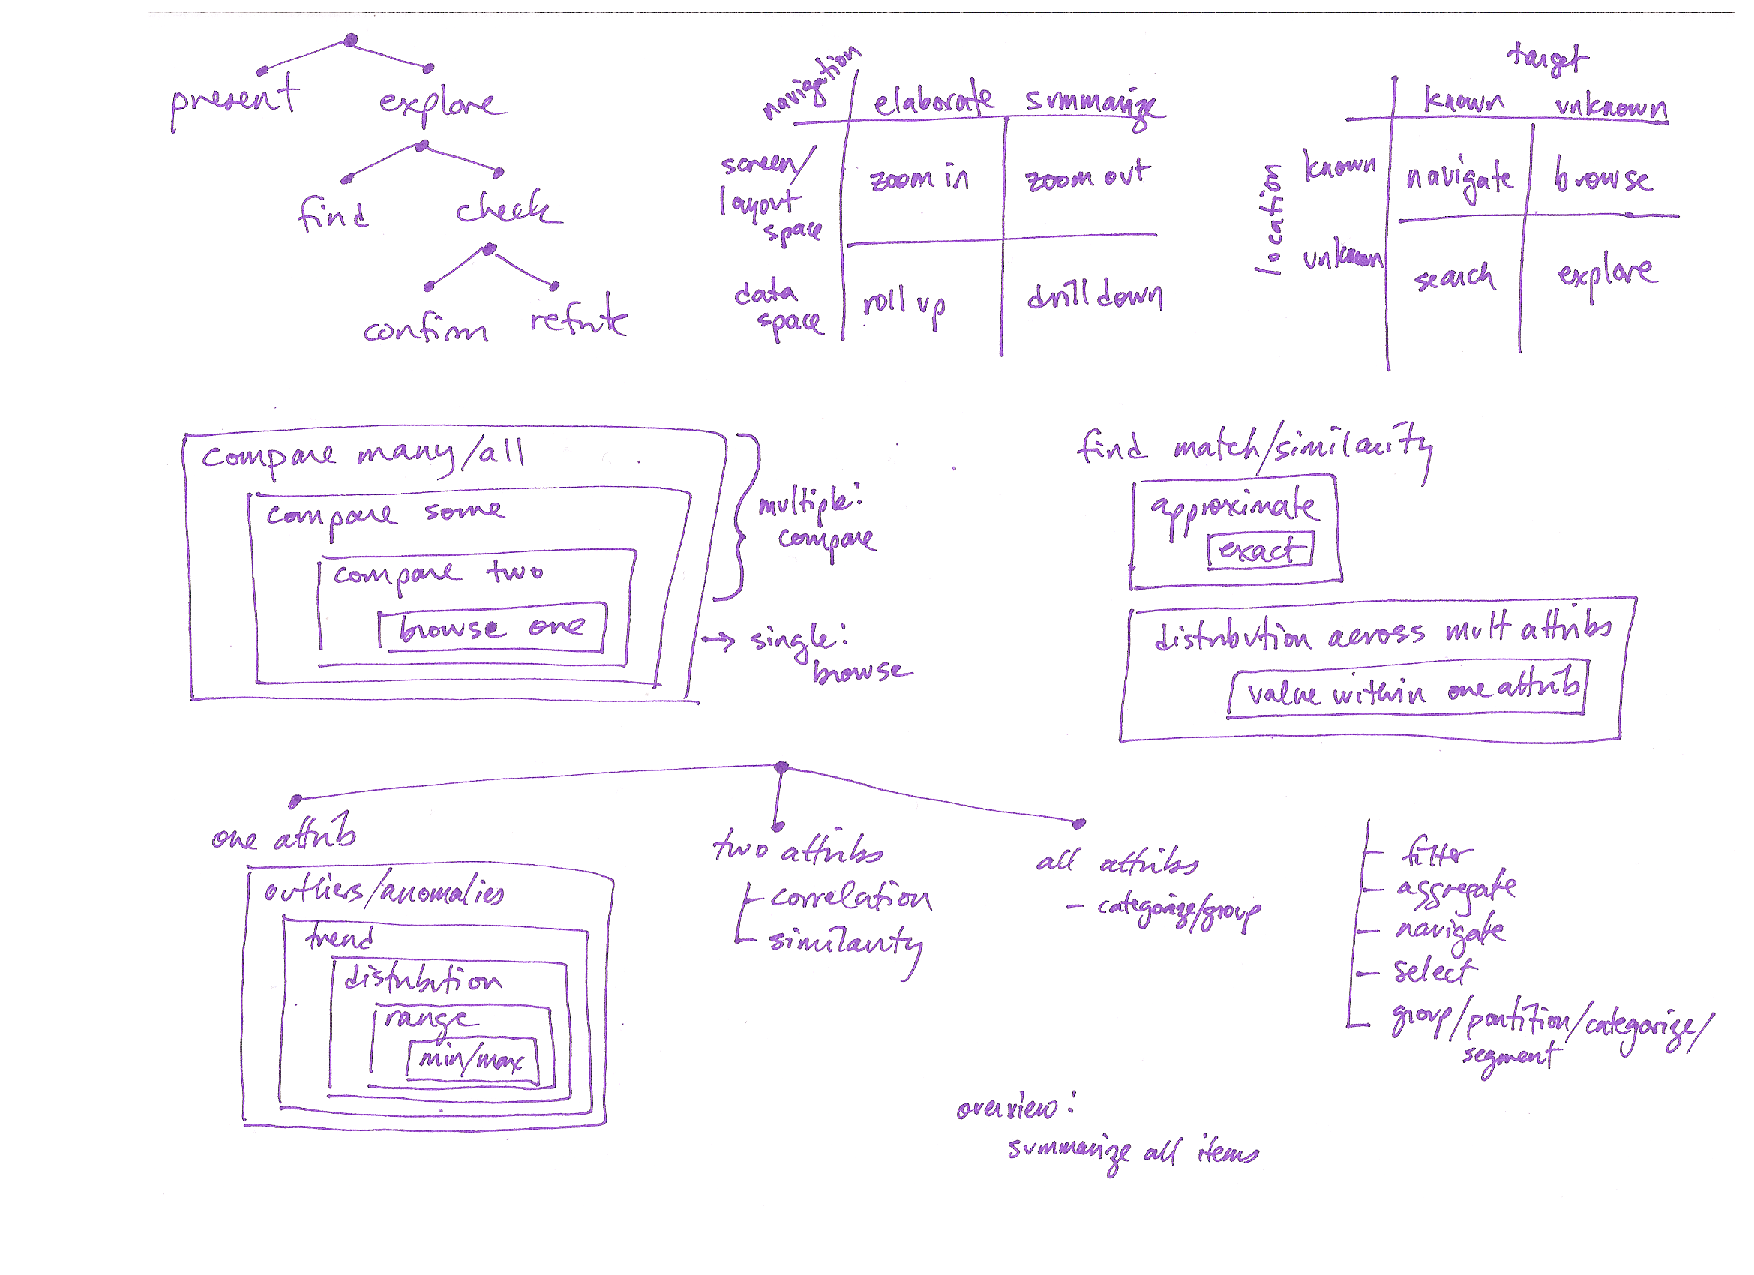
\includegraphics[width=\textwidth]{figures/typology-12-08-27-TM.pdf}
	\caption
	[
	    Early brainstorming on the topic of task classification.
	]
	{
	    {\bf August 27, 2012}: Tamara's early brainstorming on the topic of task classification.
	}
	\centering
	\label{app:typology:fig:12-08-27}
\end{figure}

%-|-|-|-|-|-|-|-|-|-|-|-|-|-|-|-|-|-|-|-|-|-|-|-|-|-|-|-|-|-|-|-|-|-|-|-|-

\refstepcounter{papernumber} 
\begin{sloppypar}
\bstart{September 11, 2012\thepapernumber}
\bibentry{Heer2012}~\cite{Heer2012}. \end{sloppypar}

\begin{quotation}
    Contributes a domain- and datatype-agnostic classification that spans low-level\index{task!low-level tasks} and high-level tasks\index{task!high-level tasks}, distinguishing between {\it data / view specification} ({\it visualize, filter, sort, derive}), {\it view manipulation} ({\it select, navigate, coordinate, organize}), and {\it process and provenance\index{analytical provenance}} ({\it record, annotate, share, guide}).
    
    One of the existing classifications that Tamara was attempting to reconcile.
\end{quotation}

\refstepcounter{papernumber} 
\begin{sloppypar}
\bstart{September 13, 2012\thepapernumber}
\bibentry{Zhou1998}~\cite{Zhou1998}. \end{sloppypar}

\begin{quotation}
    Contributes a low-level classification\index{task!low-level tasks}, distinguishing between {\it associate (collocate, connect, unite, attach), background, categorize (mark distribution), cluster (outline, individualize), compare (differentiate, intersect), correlate (plot, mark compose), distinguish (mark distribution, isolate), emphasize (focus, isolate, reinforce), generalize (merge), identify (name, portray, individualize, profile), locate (position, situate, pinpoint, outline), rank (time), reveal (expose, itemize, specify, separate), switch}, and {\it encode\index{visual encoding} (label, symbolize (quantify, iconify), portray, tabulate, plot, structure, trace, map)}.
    
    These terms can be occur in various combinations with respect to {\it inform} and {\it enable} intents. 
    The types of {\it inform} include {\it elaborate} and {\it summarize}.
    The types of enable include {\it explore} ({\it search, verify}) and {\it compute} ({\it sum, compute}).
    
    One of the existing classifications that Tamara was attempting to reconcile.
\end{quotation}

\refstepcounter{papernumber} 
\begin{sloppypar}
\bstart{September 13, 2012\thepapernumber}
\bibentry{Yi2007}~\cite{Yi2007}. \end{sloppypar}

\begin{quotation}
    Contributes a low-level classification\index{task!low-level tasks} that distinguishes between {\it select, explore, reconfigure, encode\index{visual encoding}, abstract, elaborate, filter, connect} and a category for {\it other} processes including {\it undo} and {\it redo}, {\it change configuration / layout / settings}.
    
    One of the existing classifications that Tamara was attempting to reconcile.
\end{quotation}

\refstepcounter{papernumber} 
\begin{sloppypar}
\bstart{September 18, 2012\thepapernumber}
\bibentry{Amar2005}~\cite{Amar2005}. \end{sloppypar}

\begin{quotation}
    Contributes a low-level classification\index{task!low-level tasks} that distinguishes between {\it retrieve, filter, compute derived value, find extremum, sort, determine range, characterize distribution, find anomalies, cluster}, and {\it correlate}.

    One of the existing classifications that Tamara was attempting to reconcile.
\end{quotation}

\refstepcounter{papernumber} 
\begin{sloppypar}
\bstart{September 18, 2012\thepapernumber}
\bibentry{Roth1990}~\cite{Roth1990}. \end{sloppypar}

\begin{quotation}
    Contributes a low-level classification\index{task!low-level tasks} that distinguishes between {\it value lookup, compare within a relation, compare across or between relations, determine distributions, determine correlations, indexing}, and {\it sorting}.
    
    One of the existing classifications that Tamara was attempting to reconcile.
\end{quotation}

\refstepcounter{papernumber} 
\begin{sloppypar}
\bstart{September 18, 2012\thepapernumber}
\bibentry{Wehrend1990}~\cite{Wehrend1990}. \end{sloppypar}

\begin{quotation}
    \begin{sloppypar}
    Contributes a low-level classification\index{task!low-level tasks} that includes {\it identify (lookup value), locate, distinguish, categorize, cluster (determine), distribution, rank, compare (within and between relations), associate}, and {\it correlate}.
    \end{sloppypar}
    
    One of the existing classifications that Tamara was attempting to reconcile.
\end{quotation}

\refstepcounter{papernumber} 
\begin{sloppypar}
\bstart{September 18, 2012\thepapernumber}
\bibentry{Chi1998}~\cite{Chi1998}. \end{sloppypar}

\begin{quotation}
    Contributes a low-level classification\index{task!low-level tasks}, a temporal / pipeline model of visualization construction, describing four stages interleaved with four transformations: {\it the data stage (value filtering, subsetting), data transformation (deriving, computing new attributes, aggregating), the analytical abstraction stage (select subset to visualize), visualization transformation (\eg cluster, \ac{MDS}), the visualization abstraction stage (simplify), visual mapping transformation (choose visual encoding\index{visual encoding} technique)}, and {\it the view stage (navigation, orientation, view-filter, dynamic view-filtering, brushing\index{view coordination!brushing across views}, animating\index{view coordination!animated transitions}, focus, permute)}.
\end{quotation}

\refstepcounter{papernumber} 
\begin{sloppypar}
\bstart{September 19, 2012\thepapernumber}
\bibentry{Morse2000}~\cite{Morse2000}. \end{sloppypar}

\begin{quotation}
    An example of an evaluation where the authors use the classification of \citet{Zhou1998} to evaluate four different visualization tools for information retrieval\index{information retrieval}.
     They translate a subset of this abstract classification into concrete domain tasks particular to the datasets used in the study.

    We cited this work in early drafts but not in \autoref{ch:typology} or \citet{Brehmer2013}, as we opted to cite \citet{Perer2009} as an example of an evaluation incorporating a prior classification.
\end{quotation}

\refstepcounter{papernumber} 
\begin{sloppypar}
\bstart{September 20, 2012\thepapernumber}
\bibentry{Shneiderman1996}~\cite{Shneiderman1996}. \end{sloppypar}

\begin{quotation}
    Contributes a low-level classification\index{task!low-level tasks}, distinguishing between {\it overview, zoom, filter, details-on-demand\index{view coordination!details-on-demand}, relate, history}, and {\it extract}.
    
    \begin{sloppypar}
    Also contributes a classification of tasks\index{task} by data type for one-dimensional ({\it counting, filtering, details-on-demand\index{view coordination!details-on-demand}}),
    two-dimensional (subsumes one dimensional tasks, {\it containment, compare, relate}), and three-dimensional data (subsumes one and two dimensional data tasks, {\it adjacency, understanding position and orientation, resolving occlusion}), tasks for temporal or time-oriented\index{time-oriented data} data (subsumes one-dimensional data tasks, {\it determine start / end, find overlap, find events before / after / during}), for multi-dimensional data ({\it  finding patterns of variables, gaps, outliers, resolving disorientation, occlusion}), as well as for tree-based data (subsumes one-dimensional data tasks applied to items and links, {\it determine how many levels in the tree, how many children does an item have, examine types of objects at different tree depths, examine breadth / depth}) and network data\index{network data} (subsumes tree-based data tasks, {\it examine shortest/less costly paths, network traversal}).
    \end{sloppypar}
    
    One of the existing classifications that Tamara was attempting to reconcile.
\end{quotation}

\refstepcounter{papernumber} 
\begin{sloppypar}
\bstart{September 21, 2012\thepapernumber}
\bibentry{Lam2008}~\cite{Lam2008}. \end{sloppypar}

\begin{quotation}
    Describes a survey of 484 references appearing in visualization venues and analyzed according to the {\it Seven Stages of Action} framework by \citet{Norman1988}. 
    In addition to Norman's {\it gulf of execution} and {\it gulf of evaluation}, Lam adds a {\it gulf of formation} to represent high-level cognitive decision costs related to data analysis and intent formation.
\end{quotation}

\refstepcounter{papernumber} 
\begin{sloppypar}
\bstart{September 21, 2012\thepapernumber}
\bibentry{Lee2006}~\cite{Lee2006}. \end{sloppypar}

\begin{quotation}
    \begin{sloppypar}
    Contributes a low-level classification\index{task!low-level tasks} specific to graph-based data, distinguishing between {\it topology tasks} ({\it determine adjacency, determine accessibility, find common connection, determine connectivity: shortest path, clusters, connected components, bridges, articulation points}), {\it attribute tasks} ({\it find node attributes, find link attributes}), {\it browsing tasks} ({\it follow path, revisit}), and {\it overview tasks}.
    \end{sloppypar}
    
    One of the existing classifications that Tamara was attempting to reconcile.
\end{quotation}

\refstepcounter{papernumber} 
\begin{sloppypar}
\bstart{September 25, 2012\thepapernumber}
\bibentry{Jankun-Kelly2007}~\cite{Jankun-Kelly2007}. \end{sloppypar}

\begin{quotation}
    Proposes a formal model to explain exploration with visualization tools, a formal ``{\it P-set}'' grammar for describing the model, and contributes a software framework for recording exploration. 
    The model centres around {\it parameter adjustments} and {\it transformations} that reference \citet{Card1999}, including {\it data filtering, data transformation, visual (primitive) mapping, rendering, and view transformations}.
    Claims that previous classifications by \citet{Chi1998}, \cite{Chuah1996}, \citet{Shneiderman1996}, and \citet{Wehrend1990} ``{\it focus on the goal of the user, not how the visualization was used to achieve those goals}''.

    This work was cited in our original submission but not in the  \autoref{ch:typology} or the published version of \citet{Brehmer2013}, as we also cited \citet{Card1999}, who in turn inspired the choice of elements in the {\it P-set} grammar.
\end{quotation}

\refstepcounter{papernumber} 
\begin{sloppypar}
\bstart{September 26, 2012\thepapernumber}
\bibentry{Gotz2008}~\cite{Gotz2008}. \end{sloppypar}

\begin{quotation}
    Contributes a low-level classification\index{task!low-level tasks} that distinguishes between {\it exploration}, {\it insight actions}\index{insight}, and {\it meta actions}.
    
    {\it Exploration} includes {\it data exploration} ({\it filter, inspect, query, restore}) and {\it visual exploration} ({\it brush\index{view coordination!brushing across views}, change metaphor, change range, merge, sort, split}).
    
    {\it Insight actions}\index{insight} include those related to {\it visual insight} ({\it annotate, bookmark}) and {\it knowledge insight} ({\it create, modify, remove}).
    
    {\it Meta actions} include {\it delete, edit, redo, revisit}, and {\it undo}.
\end{quotation}

\refstepcounter{papernumber} 
\begin{sloppypar}
\bstart{September 26, 2012\thepapernumber}
\bibentry{Casner1991}~\cite{Casner1991}. \end{sloppypar}

\begin{quotation}
    Contributes a low-level classification\index{task!low-level tasks}, distinguishing between {\it search operators} ({\it search, lookup, verify}) and {\it computation operators} ({\it equal, less than, greater than, plus, difference, times, quotient}).
    
    One of the existing classifications that Tamara was attempting to reconcile.
\end{quotation}

\refstepcounter{papernumber} 
\begin{sloppypar}
\bstart{September 26, 2012\thepapernumber}
\bibentry{Mullins1993}~\cite{Mullins1993}. \end{sloppypar}

\begin{quotation}
    Contributes a domain- and datatype-agnostic classification that spans low-level\index{task!low-level tasks} and high-level tasks\index{task!high-level tasks}, containing over 140 terms: an exhaustive list of high-level\index{task!high-level tasks} {\it mediation} and {\it coordination} tasks\index{task}, as well as many low-level\index{task!low-level tasks} object-oriented interactions\index{interaction} relating to physical interface input and output.
    
    Their list of {\it mediation} and {\it coordination} terms include: {\it assess} ({\it success}, {\it evaluate}, {\it test}, {\it compare}, {\it verify}), {\it analyze} ({\it interpret}, {\it calculate}, {\it categorize}, {\it count}, {\it itemize}, {\it tabulate}), {\it synthesize} ({\it integrate}, {\it translate}, {\it remember}, {\it prioritize}, {\it estimate}, {\it extrapolate}, {\it interpolate}), {\it solve problems} ({\it plan}, {\it formulate}, {\it plan}, {\it program}, {\it diagnose}, {\it decide}, {\it choose}), {\it learn} ({\it query}, {\it tutorial}, {\it browse}), {\it undo}, {\it reset}, and {\it cross-reference}.
    
    Their list of {\it object space modeling} terms include:
    {\it create} ({\it associate}, {\it name}, {\it group}, {\it link}, {\it assemble}, {\it aggregate}, {\it paste}, {\it overlay}, {\it insert}, {\it replicate}, {\it copy}, {\it instance}, {\it store}, {\it introduce}, {\it data entry}, {\it restore}), {\it eliminate} ({\it remove}, {\it cut}, {\it delete}, {\it purge}, {\it disassociate}, {\it rename}, {\it ungroup}, {\it unlink}, {\it disassemble}, {\it segregate}, {\it filter}, {\it suppress}, {\it withdraw}), {\it activate} ({\it execute a process}, {\it start}, {\it invoke}, {\it change status}, {\it re-start}, {\it foreground/background switch}, {\it stop process}, {\it suspend}, {\it terminate}, {\it set-aside}, {\it quit}), {\it indicate} ({\it pick}, {\it reference}, {\it mark}), {\it edit}, and {\it display}
    
    \begin{sloppypar}
    Their list of {\it communicate} terms include: {\it transmit} ({\it call}, {\it acknowledge}, {\it respond}, {\it suggest}, {\it direct}, {\it inform}, {\it instruct}, {\it request}, {\it record}, {\it transform}, {\it stretch}, {\it sketch}, {\it re-orient}, {\it shape}, {\it pan}, {\it zoom}, {\it move}, {\it select}, {\it position}, {\it orient}, {\it quantify}, {\it text}, {\it hold}, {\it push}, {\it pull}, {\it control}), {\it reach through}, and {\it receive} ({\it attend}, {\it monitor}, {\it notice}, {\it filter}, {\it accept}, {\it acquire}, {\it observe}, {\it scan}, {\it search}, {\it inspect}, {\it extract}, {\it screen}, {\it detect}, {\it discriminate}, {\it recognize}, {\it identify}, {\it locate}).
    \end{sloppypar}
    
    A neglected paper that Tamara pointed me to. 
\end{quotation}

\refstepcounter{papernumber} 
\begin{sloppypar}
\bstart{September 27, 2012\thepapernumber}
\bibentry{Ware2004}~\cite{Ware2004}. \end{sloppypar}

\begin{quotation}
    Contributes a high-level classification\index{task!high-level tasks}.
    In Ware's {\it Interacting with Visualizations} chapter, there are three loops of activity that define interaction with a visualization: {\it the data manipulation loop, the exploration and navigation loop}, and {\it the problem solving loop}. 
    
    In Ware's {\it Thinking with Visualizations} chapter, the {\it problem solving loop} is tangentially addressed, referencing the sensemaking\index{sensemaking} model of \citet{Pirolli2005}.
    However, this chapter mainly deals with memory models and knowledge costs, limits to visual working memory, and eye movements. 
    There is a section on {\it visual problem solving}, which breaks the process down into the following nested hierarchy: {\it problem solving, visual query, the pattern finding loop, eye movements, and intrasaccadic image-scanning}.
    
    The final section of the chapter addresses {\it creative problem solving} and {\it creative thinking} as high-level tasks, which involves stages of {\it preparation}, {\it production}, and {\it judgment}.
\end{quotation}

\refstepcounter{papernumber} 
\begin{sloppypar}
\bstart{September 28, 2012\thepapernumber}
\bibentry{Tory2004}~\cite{Tory2004}. \end{sloppypar}

\begin{quotation}
    Makes compelling or noteworthy assertions about the behaviour of people who use visualization tools or techniques.
    The authors outline the relationships between tasks\index{task} with different visualization design models. 
    Their classification of tasks breaks down into {\it whether spatialization is constrained} and whether the design model is assumed to be {\it continuous} or {\it discrete}.
    
    For a {\it continuous design model}, tasks include {\it find[ing] spatial relationships and spatial regions of interest} for a {\it given spatialization} and	{\it finding numeric trends} for a {\it chosen spatialization}.
    
    For a {\it discrete design model}, tasks can pertain to {\it values} ({\it finding patterns such as clusters and outliers}) or {\it structure} ({\it analyzing connectivity relationships}); other tasks include {\it retrieving item details and filtering or excluding items}.
\end{quotation}

\refstepcounter{papernumber} 
\begin{sloppypar}
\bstart{October 1, 2012\thepapernumber}
\bibentry{Chuah1996}~\cite{Chuah1996}. \end{sloppypar}

\begin{quotation}
    Contributes a low-level classification\index{task!low-level tasks}, which distinguishes between {\it graphical operations}, {\it set operations}, and {\it data operations}.
    
    Their list of {\it graphical operations} includes {\it encode\index{visual encoding} data} ({\it create mapping, transform mapping}), {\it set graphical value}, {\it manipulate objects} ({\it creating, copying, deleting}).
    
    Their list of {\it set operations} includes {\it create} ({\it enumerate, express membership}), {\it delete}, and {\it summarize}.
    
    Their list of {\it data operations} includes {\it add objects, delete objects}, and {\it derive attributes}.
\end{quotation}

\refstepcounter{papernumber} 
\begin{sloppypar}
\bstart{October 2, 2012\thepapernumber}
\bibentry{Plaisant1995}~\cite{Plaisant1995}. \end{sloppypar}

\begin{quotation}
    Presents a taxonomy of browser interfaces, both single-view and multiple-view variants, including overview and detail displays. 
    Contributes a high-level task\index{task!high-level tasks} classification that justifies the different browser types: {\it image generation}, {\it open-ended exploration}, {\it diagnostic}, {\it navigation}, and {\it monitoring}.
\end{quotation}

\refstepcounter{papernumber} 
\begin{sloppypar}
\bstart{October 3, 2012\thepapernumber}
\bibentry{Roth2012a}~\cite{Roth2012a}. \end{sloppypar}

\begin{quotation}
    Contributes a meta-analysis of interaction\index{interaction} taxonomies and classifications in the visualization and cartographic\index{cartography} literature, distinguishing these prior classifications by referring to \citet{Norman1988} and his terms {\it  objective (intents)}, {\it operator (tools/widgets)}, and {\it operand (data objects/abstractions)} from his {\it Stages of Action} model.
    
    Roth's meta-analysis partially overlaps with our own: he includes the classifications of \citet{Amar2005}, \citet{Buja1996}, \citet{Chi1998}, \citet{Chuah1996}, \citet{Dix1998}, \citet{Keim2002}, \citet{Shneiderman1996}, \citet{Ward2004}, \citet{Wehrend1990}, \citet{Yi2007}, and \citet{Zhou1998}.
    His meta-analysis also includes 13 other classifications, largely from the geovisualization and cartographic literature\index{cartography}.
    
    Roth identifies several concordances and differences across the classifications that he surveyed: the terms {\it identify} and {\it compare} are the most common; most {\it objective}-oriented classifications are at a high-level of abstraction; {\it objective} and {\it operator} classifications are often hard to delineate; {\it brushing}\index{view coordination!brushing across views} is the most common {\it operator}, {\it focusing} is defined in many different ways, there is ambiguity related to {\it changing or altering the encoding\index{visual encoding} or symbolization}; {\it viewpoint operators} are related to {\it distortion, navigation, observer motion, object rotation, panning, re-centring, re-projecting, viewpoint manipulation, and zooming}; {\it operand} classifications vary between being {\it type-centric} and {\it state-centric}, while others vary between {\it data operands} and {\it representation operands}.
\end{quotation}

\refstepcounter{papernumber} 
\begin{sloppypar}
\bstart{October 4, 2012\thepapernumber}
\bibentry{Tukey1977}~\cite{Tukey1977}. \end{sloppypar}

\begin{quotation}
    Makes compelling or noteworthy assertions about {\it exploratory data analysis}, described as being more than descriptive statistics, it requires flexibility and an attitude a ``{\it willingness to look for what can be seen}''. 
    {\it Confirmatory data analysis} can be automated, but it depends upon {\it exploratory data analysis}.
\end{quotation}

\refstepcounter{papernumber} 
\begin{sloppypar}
\bstart{October 4, 2012\thepapernumber}
\bibentry{Shrinivasan2008}~\cite{Shrinivasan2008}. \end{sloppypar}

\begin{quotation}
     Contributes a high-level classification\index{task!high-level tasks} that distinguishes between {\it externalizing evidence, hypotheses, assertions, and causal links, organizing evidence to support/refute a claim, reviewing and revising the exploration process, linking externalized evidence to support claims}, and {\it presenting findings}.
     
    The focus of this paper is on {\it visualization history tracking} and {\it knowledge externalization}.
    History and knowledge externalization can involve artefacts such as screen shots, annotations, lists of bookmarked elements or locations, parameter settings, or interaction logs\index{interaction!interaction logs}.
\end{quotation}

\refstepcounter{papernumber} 
\begin{sloppypar}
\bstart{October 5, 2012\thepapernumber}
\bibentry{Dou2009}~\cite{Dou2009}. \end{sloppypar}

\begin{quotation}
    The authors conducted a study in which a team of four volunteers qualitatively coded interaction logs\index{interaction!interaction logs} of a visual analytics\index{visual analytics} tool for financial data, a tool they were familiar with: they interactions\index{interaction} they coded were grouped into three categories: {\it finding}, {\it strategy}, and {\it method}.
    
    This work was cited in our original submission but not in the  \autoref{ch:typology} or the published version of \citet{Brehmer2013}, as we opted to refer to \citet{Shrinivasan2008} in our discussion of interaction logs\index{interaction!interaction logs}.
\end{quotation}

\refstepcounter{papernumber} 
\begin{sloppypar}
\bstart{October 10, 2012\thepapernumber}
\bibentry{Rensink2014} (Pre-print version)~\cite{Rensink2014}. \end{sloppypar}

\begin{quotation}
    Rensink discusses prospects for a science of visualization with regards to {\it low-level visual perception tasks}\index{perception}, borrowing experimental methodologies from vision science but retaining stimuli and visual tasks from the visualization domain, which include: {\it perception of correlation, pattern detection, cluster detection, outlier detection, grouping, finding convex hull of points, following a curve, finding point of maximum intensity}. 

    Rensink proposes an {\it extended vision thesis} and an {\it optimal reduction thesis}. 
    The former refers to the viewer and visualization system as a single system. 
    The latter refers to reducing a task\index{task} to low-level operations in the extended systems (low-level visual tasks that do not involve interactivity).

    % We cited this work in early drafts but not in \autoref{ch:typology} or \citet{Brehmer2013}.
    % In retrospect, the connection from our task typology to the vision science literature could have been stronger, and this reference could have helped in this regard.
\end{quotation}

\bstart{October 14--19, 2012}
I attended the 2012 IEEE VIS Conference and the 2012 ACM Workshop on Beyond time and Errors: novel evaLuation methods for Information Visualization (BELIV).
Some discussion at BELIV included arguments against task classification: that tasks\index{task} are nonlinear systems, and that new contexts, new data types, and changes of scale result in new tasks all the time; further complexity is added with collaborative tasks and tasks spread over multiple tools.

I also noted several papers of potential relevance at InfoVis/VAST~\cite{Cottam2012,Crouser2012,Lee2012,Pohl2012}, and at BELIV~\cite{Gleicher2012,Mcnamara2012} which I would add to our literature review and meta analysis over the next few months.

\refstepcounter{papernumber} 
\begin{sloppypar}
\bstart{October, 2012\thepapernumber}
\bibentry{Gleicher2012}~\cite{Gleicher2012}. \end{sloppypar}

\begin{quotation}
    This position paper asks whether evaluation (of a visualization tool / technique) is necessary.
    The results of an evaluation should be {\it actionable} and {\it persuasive}.

    We cited this work in early drafts but not in \autoref{ch:typology} or \citet{Brehmer2013}, as our claim that we had developed an {\it actionable} and {\it persuasive} classification was disputed by readers of early drafts, as discussed below.
\end{quotation}

\refstepcounter{papernumber} 
\begin{sloppypar}
\bstart{November 13, 2012\thepapernumber}
\bibentry{Pohl2012}~\cite{Pohl2012}. \end{sloppypar}

\begin{quotation}
    Contributes a meta-analysis of cognitive science theories and frameworks that can explain visual analysis using visualization tools and techniques, including {\it sensemaking}\index{sensemaking} (see our discussion of \citet{Pirolli2005}, \citet{Pirolli2009}, and \citet{Klein2006}), {\it Gestalt theory}, {\it distributed cognition}\index{distributed cognition} (see our discussion of \citet{Hollan2000}, \citet{Liu2008}, and \citet{Kirsh1994}), {\it graph comprehension} (see our discussion of \citet{Friel2001}) and {\it skill-rule knowledge theories}. 
    
    They indicate whether (and the degree to which) these theories or frameworks help to explain {\it preattentive processing, tool and mapping comprehensibility, visual pattern detection, open data exploration, the solving of ill-defined and well-defined problems, interaction\index{interaction} strategies, interpretation, hypothesis generation and testing, insights\index{insight}, sensemaking\index{sensemaking}, decision making, operationalizability, errors}, and {\it collaboration}.
\end{quotation}

%-------------------------------------------------------------------------

\section{Meta-Analysis of Existing Classifications}
\label{app:typology:meta-analysis}

%-------------------------------------------------------------------------

\bstart{November 2012 -- January 2013}
After surveying the sources listed up until this point, Tamara and I began to characterize the dimensions and foci of existing classifications (Figures~\ref{app:typology:fig:high-mid-low} and~\ref{app:typology:fig:domain-vs-interface} and \autoref{app:typology:table:survey}).
These figures are culled from eight slide presentations generated between November 2012 and March 2013\footnote{489 slides in total, with an average of 60 slides per presentation.}, as a slide presentation was the primary medium in which we consolidated, framed, refined, and commented on our ideas. 

This meta-analysis eventually culminated in the discussion in \autoref{typology:rw} and in \autoref{typology:tab:rw:why} and \autoref{typology:tab:rw:how}.

\autoref{app:typology:fig:high-mid-low} indicates some of the dimensions considered in this meta-analysis of existing classifications, along with examples of high-level\index{task!high-level tasks}, mid-level\index{task!mid-level tasks}, and low-level tasks\index{task!low-level tasks}.
These dimensions refer to the domains interested in studying the tasks, the domain-specificity of the task, the linearity of the task, whether the tasks can be performed with variation from person to person, how the tasks could be studied, and how these tasks are supported.

Meanwhile, \autoref{app:typology:fig:domain-vs-interface} presents another view of our meta-analysis, in which our notion of ``mid-level tasks'' are described as being interface- and domain-independent.

\autoref{app:typology:table:survey} summarizes the metadata associated with existing classifications, which included bibliographic information, the depth or number of hierarchical levels in the particular classification, and meta-classifications terms originating with \citet{Roth2012a} and \citet{Chuah1996}, as well as the method or means by which the classification was developed.

I also continued to consult additional literature during this period.

%-|-|-|-|-|-|-|-|-|-|-|-|-|-|-|-|-|-|-|-|-|-|-|-|-|-|-|-|-|-|-|-|-|-|-|-|-

\begin{figure}
	\centering
	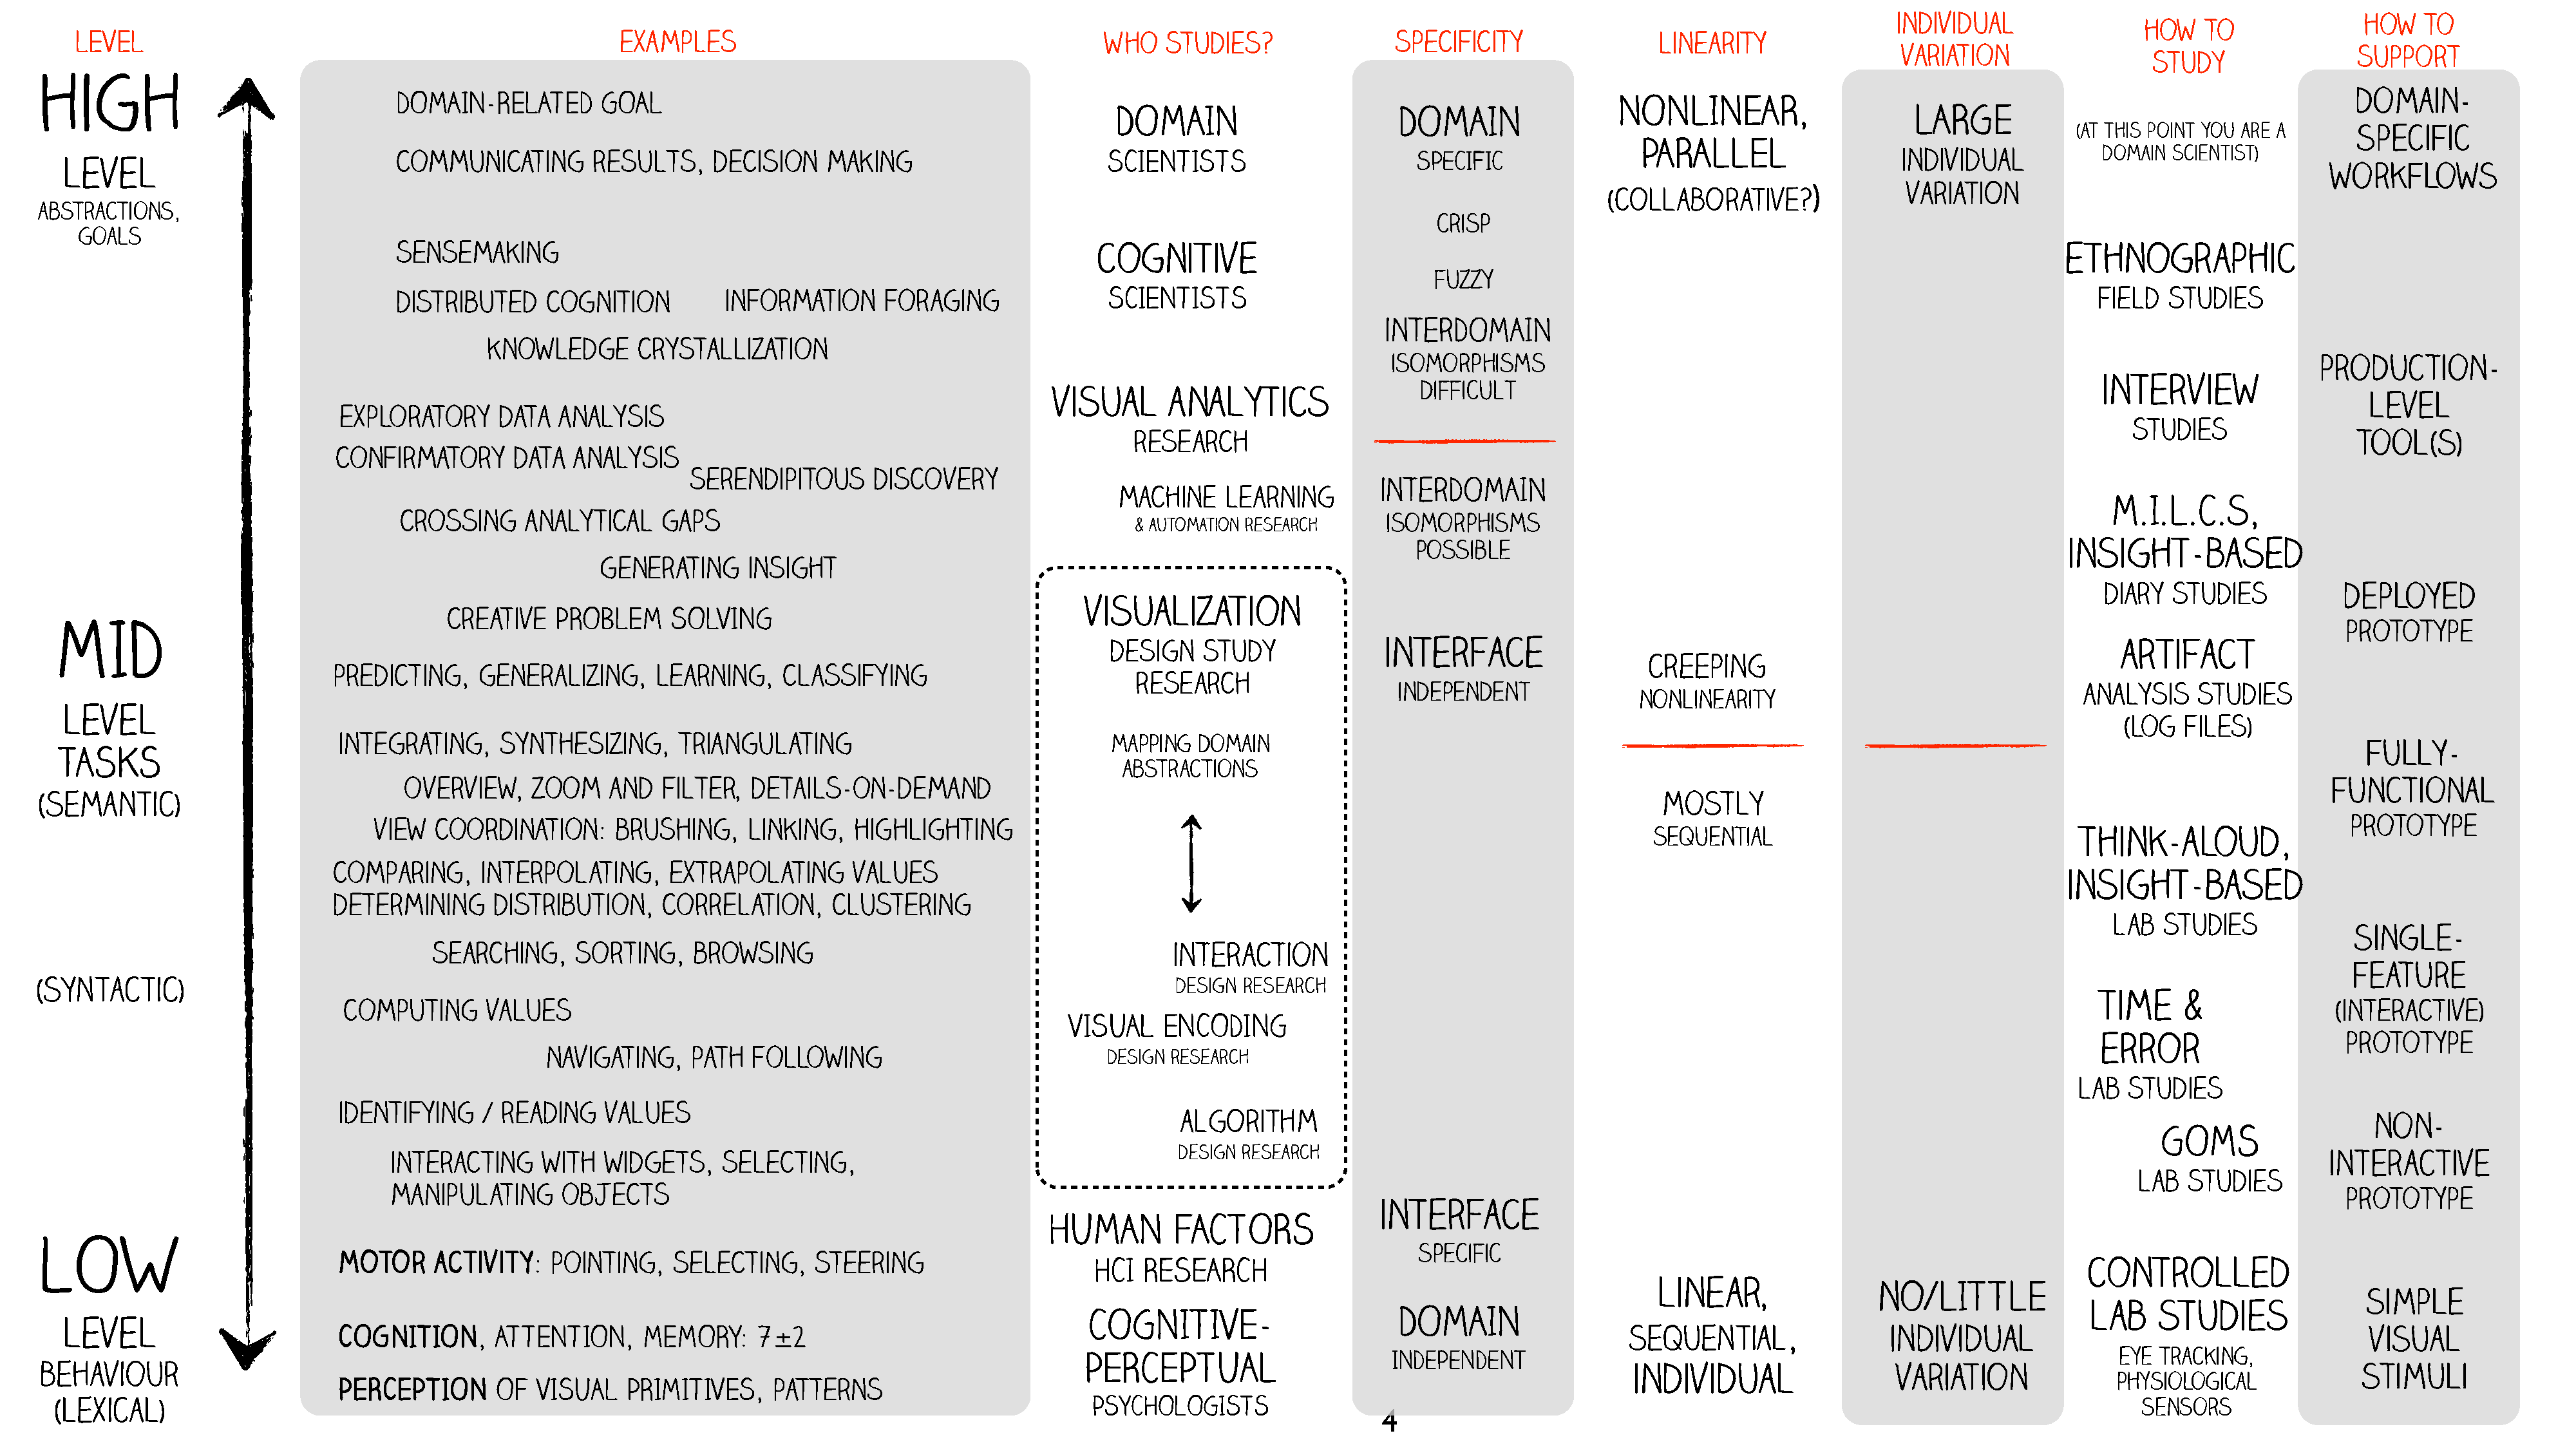
\includegraphics[width=\textwidth]{figures/typology-high-mid-low.pdf}
	\caption
	[
	    Dimensions of high-level, mid-level, and low-level tasks.
	]
	{
	    {\bf November 14, 2012}: Cross-cutting dimensions of high-level, mid-level, and low-level tasks: who studies them, their specificity, their linearity, individual variation, how they could be studied, and how these tasks are supported.
	}
	\centering
	\label{app:typology:fig:high-mid-low}
\end{figure}

%-|-|-|-|-|-|-|-|-|-|-|-|-|-|-|-|-|-|-|-|-|-|-|-|-|-|-|-|-|-|-|-|-|-|-|-|-

%-|-|-|-|-|-|-|-|-|-|-|-|-|-|-|-|-|-|-|-|-|-|-|-|-|-|-|-|-|-|-|-|-|-|-|-|-

\begin{figure}
	\centering
	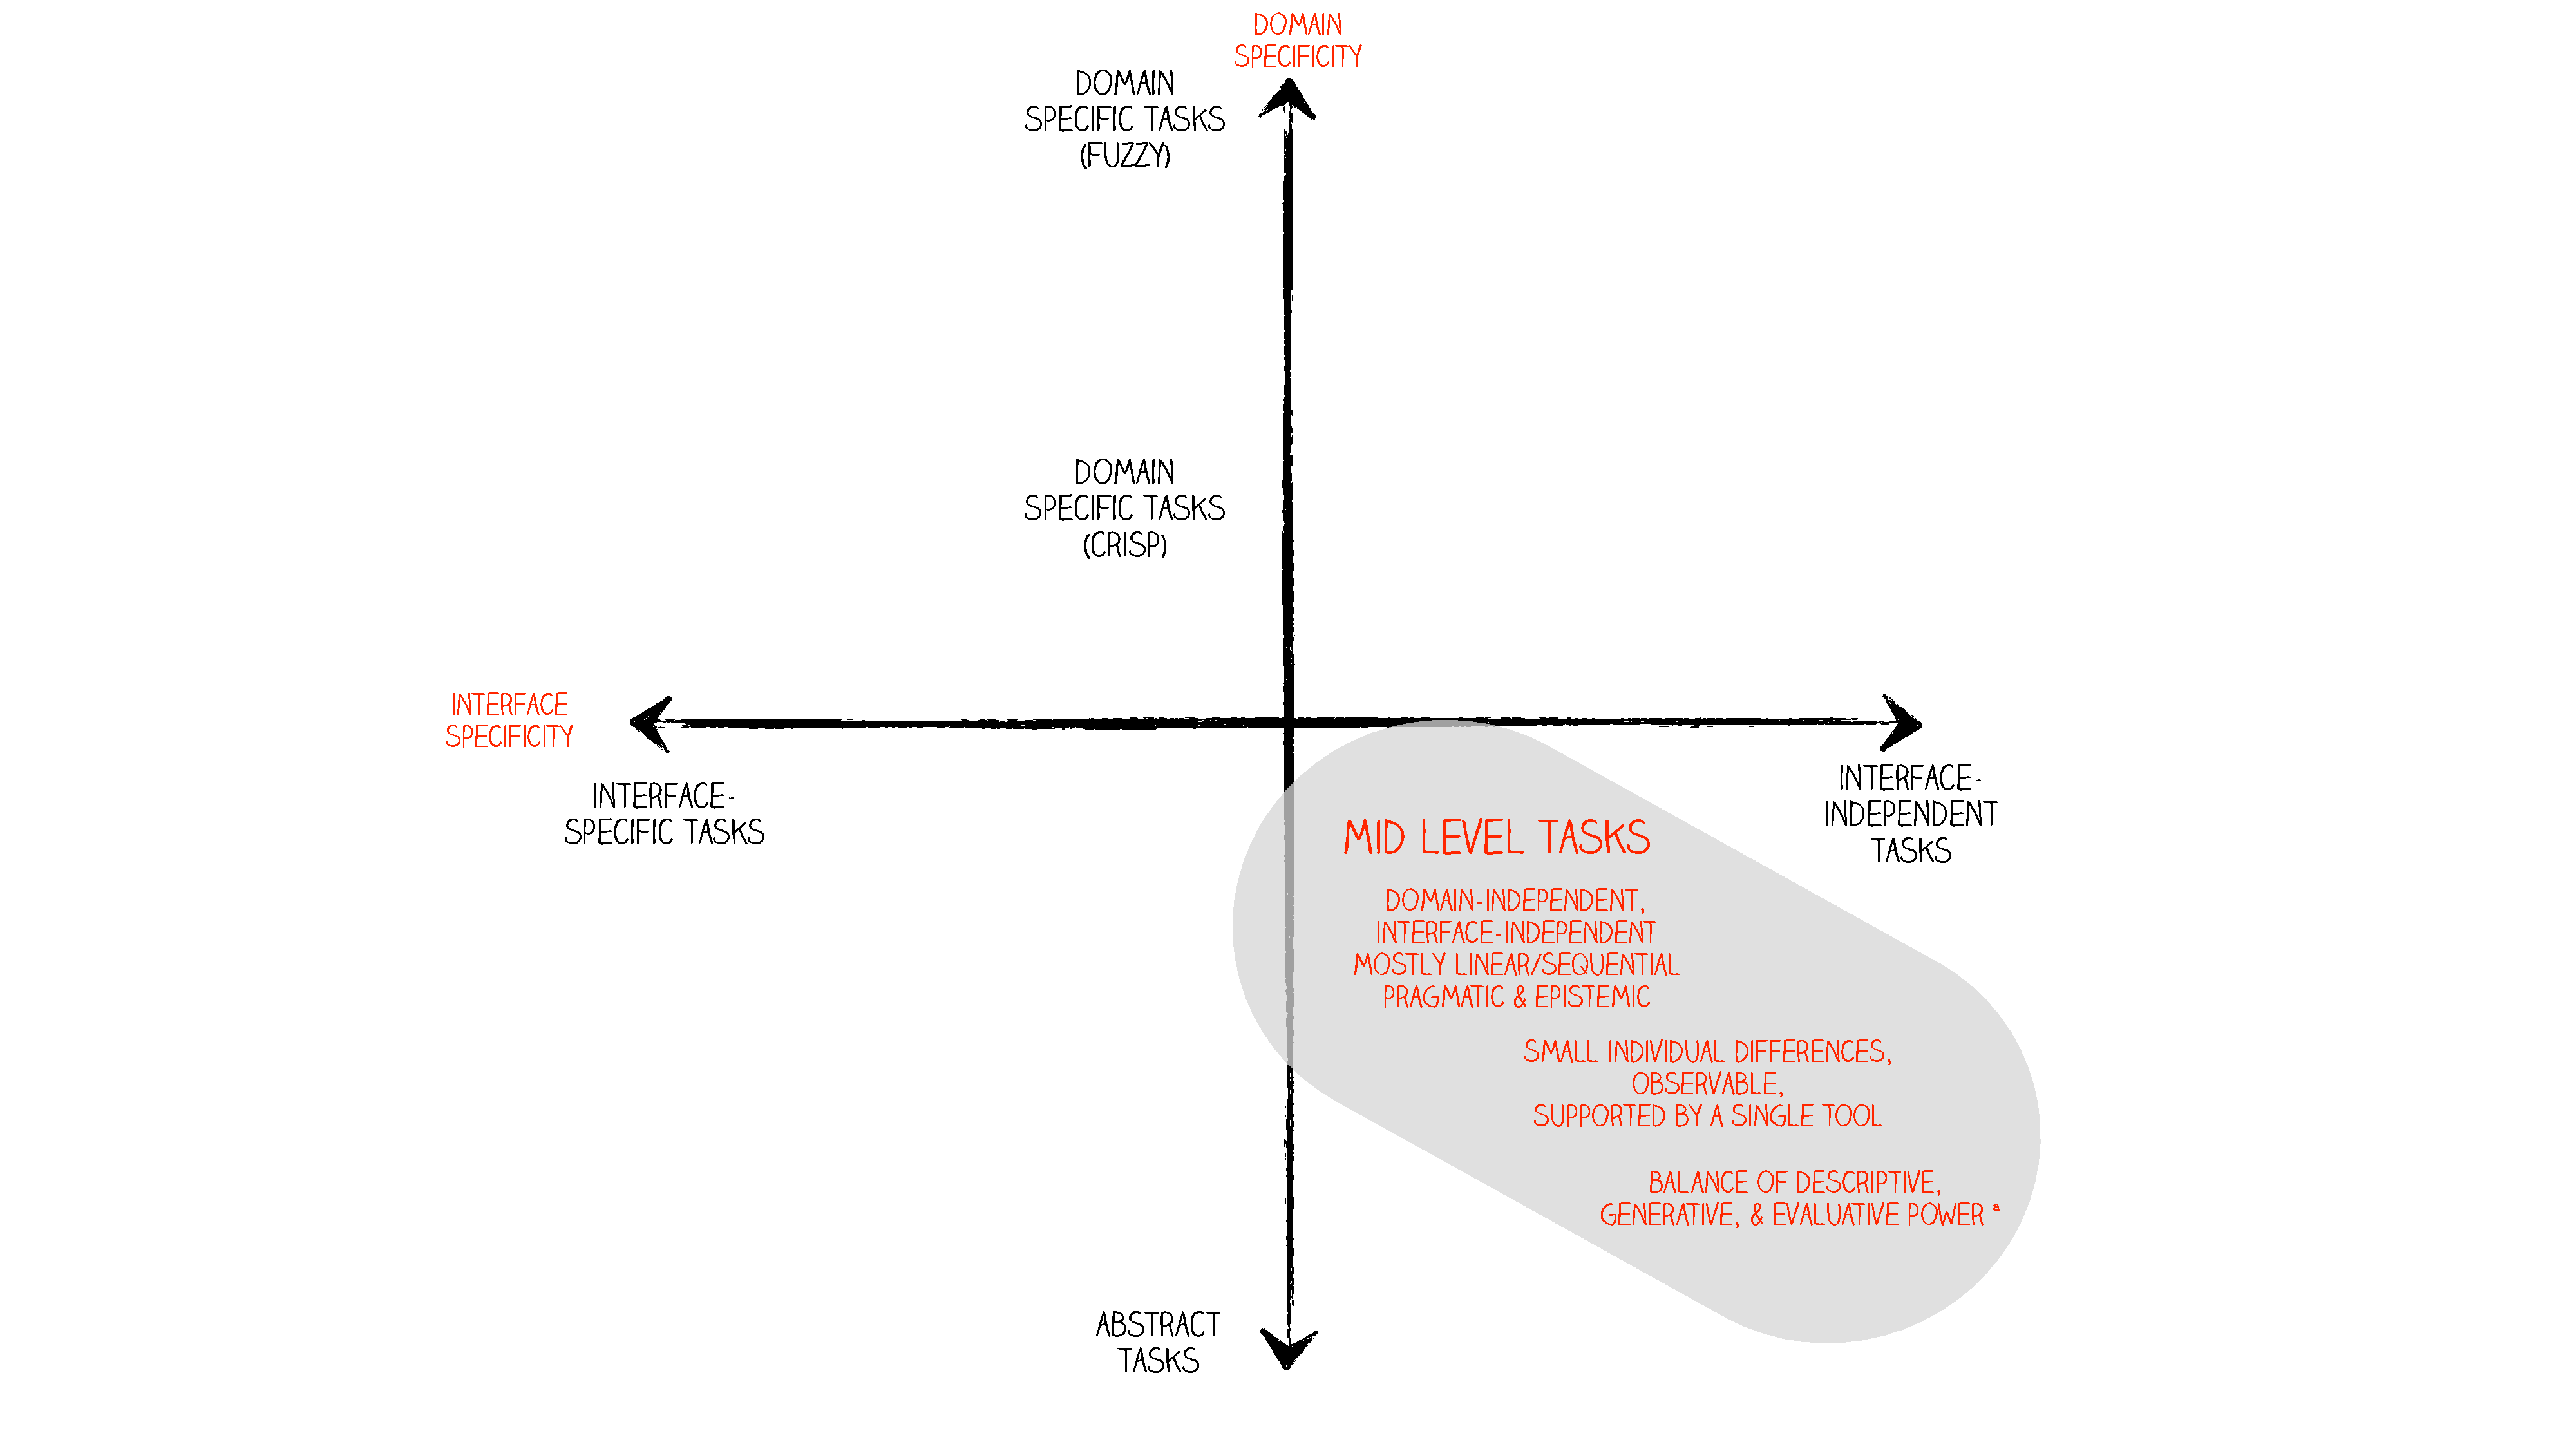
\includegraphics[width=\textwidth]{figures/typology-domain-vs-interface.pdf}
	\caption
	[
	    Mid-level abstract tasks along the axes of domain specificity and interface specificity.
	]
	{
	    {\bf November 14, 2012}: Mid-level abstract tasks along the axes of domain specificity and interface specificity.
	}
	\centering
	\label{app:typology:fig:domain-vs-interface}
\end{figure}

%-|-|-|-|-|-|-|-|-|-|-|-|-|-|-|-|-|-|-|-|-|-|-|-|-|-|-|-|-|-|-|-|-|-|-|-|-

%-|-|-|-|-|-|-|-|-|-|-|-|-|-|-|-|-|-|-|-|-|-|-|-|-|-|-|-|-|-|-|-|-|-|-|-|-

\begin{table}
	\centering
	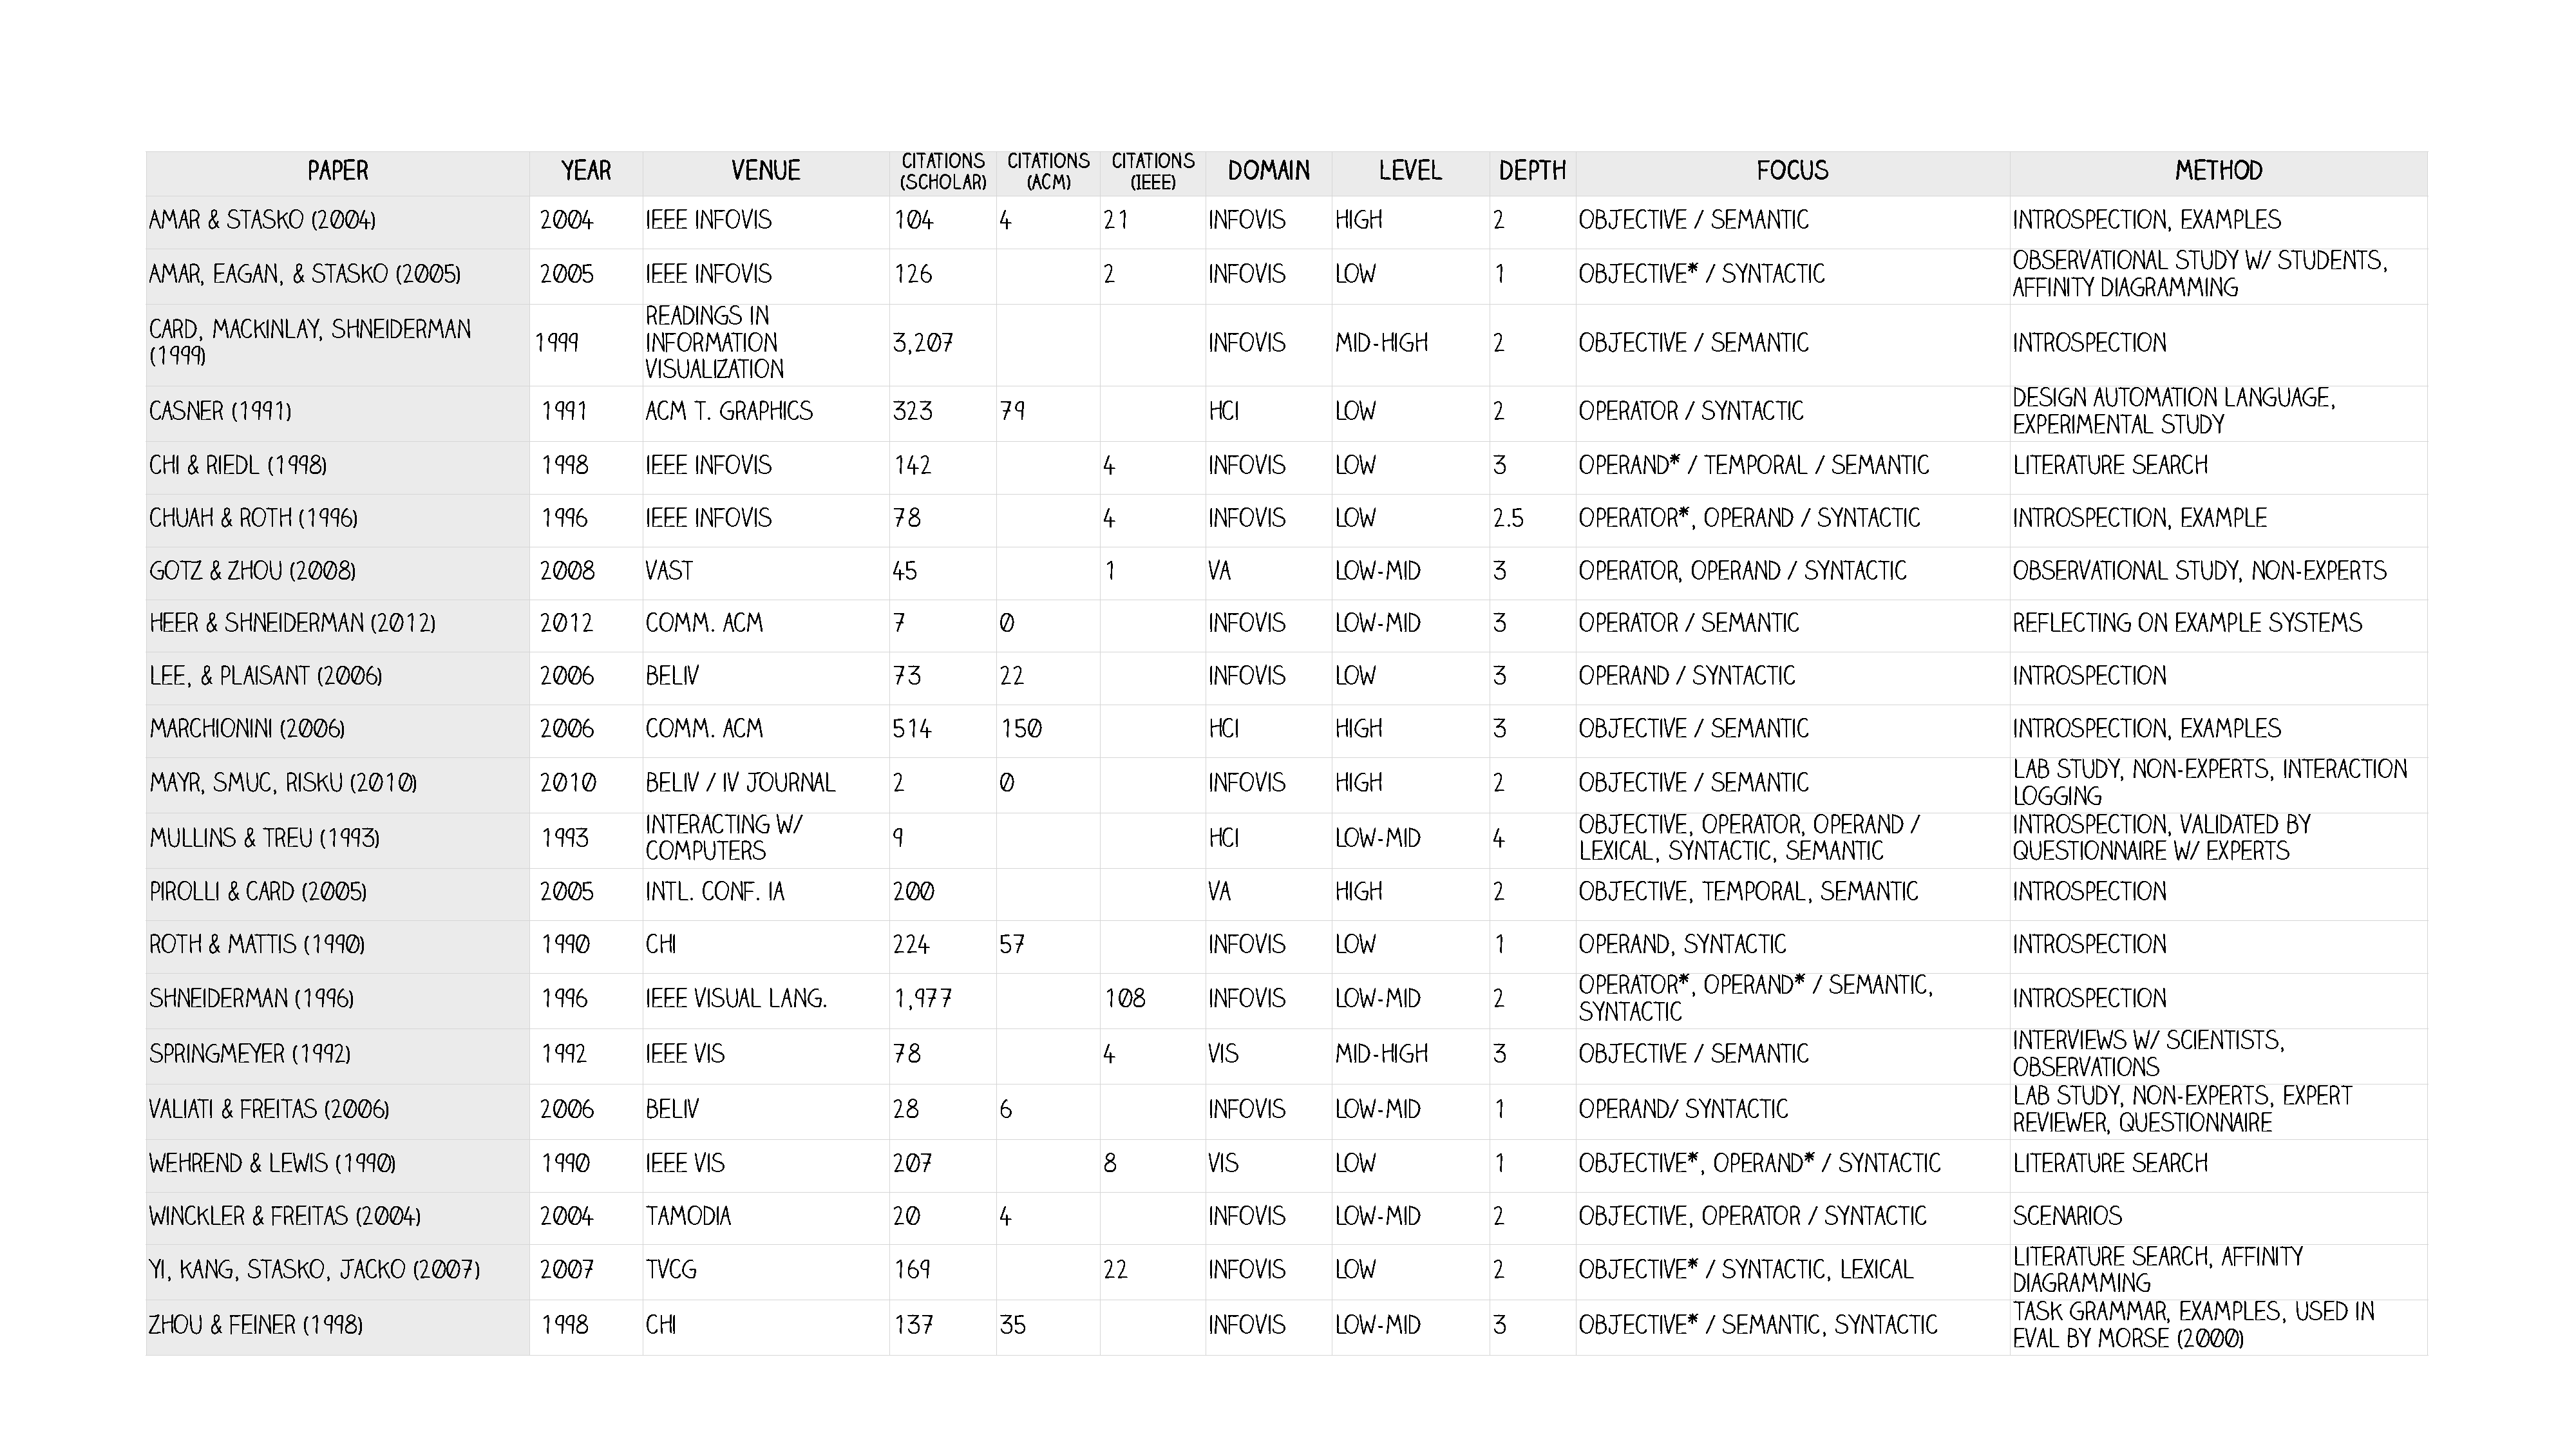
\includegraphics[width=\textwidth]{figures/typology-survey.pdf}
	\caption
	[
	    Additional dimensions of previous classifications.
	]
	{
	    {\bf November 14, 2012}: Additional dimensions of previous classifications. Citation counts are as of December 2012. Level pertains to the degree of abstraction. Depth pertains to the number of hierarchical levels in the particular classification. Asterisks in the focus column represent a classification by \citet{Roth2012a}; semantic and syntactic are terms used by \citet{Chuah1996}. Method pertains to how the particular classification was developed.
	}
	\centering
	\label{app:typology:table:survey}
\end{table}

%-|-|-|-|-|-|-|-|-|-|-|-|-|-|-|-|-|-|-|-|-|-|-|-|-|-|-|-|-|-|-|-|-|-|-|-|-

\refstepcounter{papernumber} 
\begin{sloppypar}
\bstart{November 21, 2012\thepapernumber}
\bibentry{Cottam2012}~\cite{Cottam2012}. \end{sloppypar}

\begin{quotation}
    Discuses visualization tools and technique that involve dynamic (\ie changing) data, introduces a vocabulary for quantifying {\it dynamic change}: {\it identity preserving transformations, transitional transformations, and immediate transformations}, where the type of transformation depends on the task\index{task}.
    
    We did not cite this work in \autoref{ch:typology} or \citet{Brehmer2013}, as this classification pertains more to the design space of transformation techniques and not to tasks or interactions\index{interaction}.
\end{quotation}

\refstepcounter{papernumber} 
\begin{sloppypar}
\bstart{November 21, 2012\thepapernumber}
\bibentry{Crouser2012}~\cite{Crouser2012}. \end{sloppypar}

\begin{quotation}
    \begin{sloppypar}
    Contributes an affordance-based framework for mixed-initiative systems (human-computer collaboration systems), distinguishing human affordances and machine affordances, choosing not to take a task-centric or deficiency-centric approach to constructing the framework. 
    In other words, rather than allocate tasks to a human because a computer cannot do it (computationally intractable), their framework takes the view that tasks should be allocated to the human because a human is good at it. 
    The authors recognize that humans adapt and can learn complex tasks. Humans and computers should leverage the affordances of the other for harmonious cooperation and problem-solving.
    \end{sloppypar}
    
    \begin{sloppypar}
    Human affordances include {\it visual perception\index{perception}, visuospatial thinking, audiolinguistic ability, sociocultural awareness, creativity}, and {\it domain expertise}.
    \end{sloppypar}
    
    Machine affordances include {\it large-scale data manipulation, collecting and storing large amounts of data, efficient data movement, bias-free analysis}.
    
    The framework can be used for guiding function (\ie task) allocation: to the human, to the computer, or split between both. 
    The authors state: ``{\it We need to to develop a set of canonical actions that humans can perform with known complexity, but compiling this list is nontrivial}''.

    We did not cite this work in \autoref{ch:typology} or \citet{Brehmer2013}, as we opted to focus on processes ({\ie verbs}) rather than the characteristics of the actors performing these processes.
\end{quotation}

\refstepcounter{papernumber} 
\begin{sloppypar}
\bstart{November 21, 2012\thepapernumber}
\bibentry{Mcnamara2012}~\cite{Mcnamara2012}. \end{sloppypar}

\begin{quotation}
    A position paper distinguishing between general forms of {\it analytics} and specific forms of {\it analysis}, informed by interviews with 18 intelligence analysts\index{intelligence analysis}.

    We did not cite this position paper in \autoref{ch:typology} or \citet{Brehmer2013}.
\end{quotation}

%-------------------------------------------------------------------------

\section{Our Initial Classifications of Tasks}
\label{app:typology:chronology:initial}

%-------------------------------------------------------------------------

\bstart{November 2012 -- February 2013}
At this point, Tamara and I had examined the vocabulary and definitions used in the existing classifications that we had surveyed.
Our meta-analysis reflected a top-down perspective, in which we had established the dimensions on which we could distinguish prior classifications.
However, this process did not yield our own classification of tasks\index{task}; to do so, we tried for a bottom-up approach, in which we would begin with a small set of existing classifications and gradually add and combine similar terms and remove redundant or duplicate terms, and we would continue to do so we considered additional classifications and the definitions that their authors had provided for the terms they contained.
we relied upon affinity diagramming\index{affinity diagramming} using tools such as OmniGraffle\footnote{\url{https://omnigroup.com/omnigraffle}}, Keynote\footnote{\url{http://apple.com/mac/keynote/}}, as well as post-its and whiteboards.
The diagrams and images that follow appeared throughout the eight slide presentations mentioned in \autoref{app:typology:meta-analysis}.
We began by consolidating the classifications of \citet{Heer2012}, \citet{Springmeyer1992}, \citet{Amar2005}, \citet{Gotz2008}, and \citet{Chuah1996}, as shown in \autoref{app:typology:fig:12.11.21}.

At this point, our notion of an ideal {\it task taxonomy} was one that describes tasks\index{task} at a middle level of abstraction, is domain- and interface-independent, focusing on the semantics of tasks (their objective or intent) and their temporal or sequential dependencies.
Such as taxonomy would have {\it descriptive}, {\it evaluative}, and {\it generative} power~\cite{Beaudouin-Lafon2004}, providing {\it actionable} and {\it persuasive} guidance~\cite{Gleicher2012} for visualization design and evaluation.
Our plan was to translate existing classifications into a semantic and objective language (\ie the active voice, a stance encouraged in qualitative data analysis and grounded theory\index{grounded theory} in particular~\cite{Charmaz2006}), identify emergent patterns following this translation, and attempt to map root nodes of low-level classifications to the leaf nodes of high-level classifications.

%-|-|-|-|-|-|-|-|-|-|-|-|-|-|-|-|-|-|-|-|-|-|-|-|-|-|-|-|-|-|-|-|-|-|-|-|-

\begin{figure}
	\centering
	\includegraphics[width=0.625\textwidth]{figures/typology-12-11-21.pdf}
	\caption
	[
	    Our first classification.
	]
	{
	    {\bf November 21, 2012}: Our first  classification, originating from ``data analysis'' and consolidating existing terms used by \citet{Heer2012} (orange), \citet{Springmeyer1992} (yellow), \citet{Amar2005} (blue), \citet{Gotz2008} (green), and \citet{Chuah1996} (pink).
	}
	\centering
	\label{app:typology:fig:12.11.21}
\end{figure}

%-|-|-|-|-|-|-|-|-|-|-|-|-|-|-|-|-|-|-|-|-|-|-|-|-|-|-|-|-|-|-|-|-|-|-|-|-

Through multiple rounds of coding\index{coding (qualitative data analysis)}, we continued to group similar terms and consider additional classifications, we selected representative terms for each group, and we arranged these representative terms into multiple levels of abstraction. 
This process is reflected in \autoref{app:typology:fig:12.11.23}, \autoref{app:typology:fig:12.11.28-whiteboard}, and \autoref{app:typology:fig:12.11.30}.
In our second classification, (\autoref{app:typology:fig:12.11.23}), we considered an reorganization around {\tt explore} and ``provenance\index{analytical provenance} tasks'' (the latter referring mostly to data and process management, inspired by the {\it process and provenance\index{analytical provenance}} classification by \citet{Heer2012}).
In both cases, leaf nodes pointed to operands (aspects of the data or view).
This reorganization also reflects a hybrid between the bottom-up approach reflected in \autoref{app:typology:fig:12.11.21} and the high-level top-down thinking reflected in Tamara's early proposal (see \autoref{app:typology:fig:12-08-27}).
% This section documents these multiple rounds of coding\index{coding (qualitative data analysis)} with diagrams reflecting the evolution of our typology (Figures~\ref{app:typology:fig:12.11.21} --~\ref{app:typology:fig:13.03.13}).

In our third classification (\autoref{app:typology:fig:12.11.30}), we introduced the questions of {\it why} (ends, objectives, goals), {\it what} (operands), {\it which} (also referring to operands), and {\it how} (means, methods, operators); we also considered the special case of {\it search}.
The objective, operator, and operand language is attributed to \citet{Norman1988}, which had also inspired a meta-analysis of cartographic interaction\index{interaction} classifications by \citet{Roth2012a}\index{cartography}.

%-|-|-|-|-|-|-|-|-|-|-|-|-|-|-|-|-|-|-|-|-|-|-|-|-|-|-|-|-|-|-|-|-|-|-|-|-

\begin{figure}
	\centering
	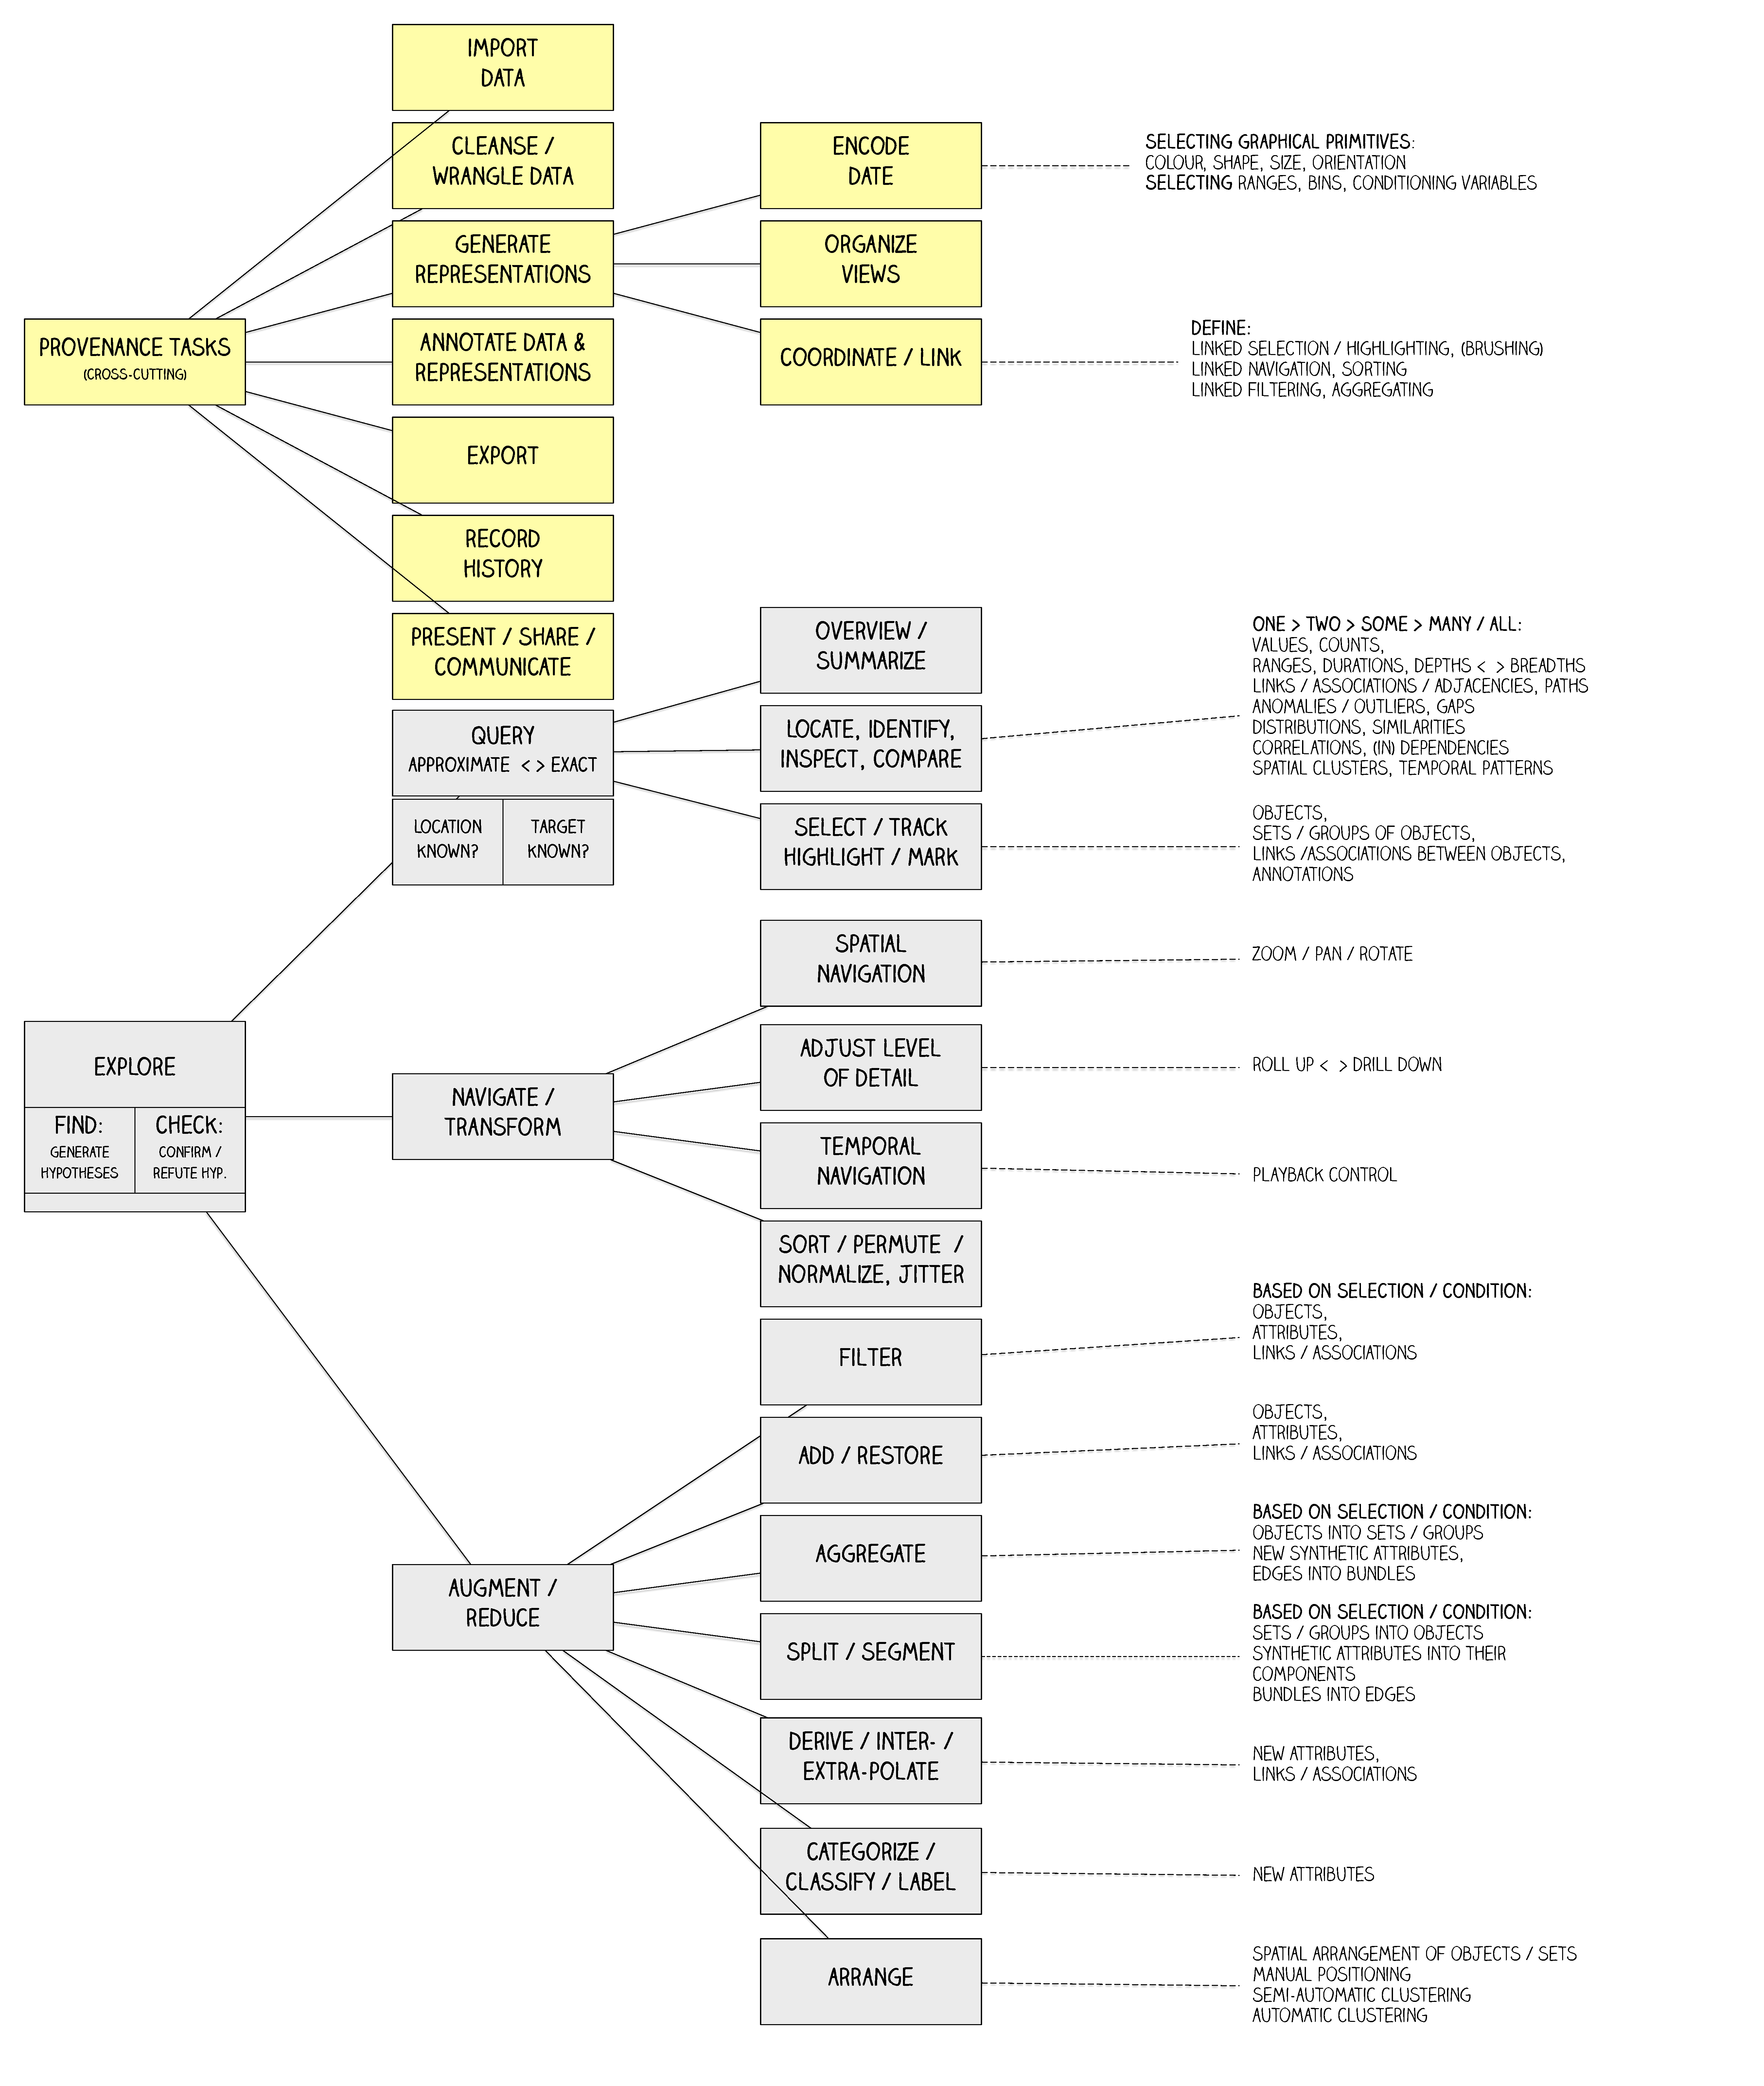
\includegraphics[width=\textwidth]{figures/typology-12-11-23.pdf}
	\caption
	[
	    Our second classification.
	]
	{
	    {\bf November 23, 2012}: Our second classification, reorganizing terms and distinguishing between ``provenance tasks'' and {\tt explore}.
	}
	\centering
	\label{app:typology:fig:12.11.23}
\end{figure}

%-|-|-|-|-|-|-|-|-|-|-|-|-|-|-|-|-|-|-|-|-|-|-|-|-|-|-|-|-|-|-|-|-|-|-|-|-

%-|-|-|-|-|-|-|-|-|-|-|-|-|-|-|-|-|-|-|-|-|-|-|-|-|-|-|-|-|-|-|-|-|-|-|-|-

\begin{figure}
	\centering
	\includegraphics[width=\textwidth]{figures/typology-12-11-28-whiteboard.pdf}
	\caption
	[
	    Whiteboard and post-it diagramming prior to our third classification
	]
	{
	    {\bf November 26--28, 2012}: Whiteboard and post-it diagramming prior to our third classification reflecting the influence of \citet{Roth2012} (and \citet{Norman1988}, indirectly), reflecting an organization around operands (top right), objectives (bottom right), and temporal dependencies (bottom left).
	}
	\centering
	\label{app:typology:fig:12.11.28-whiteboard}
\end{figure}

%-|-|-|-|-|-|-|-|-|-|-|-|-|-|-|-|-|-|-|-|-|-|-|-|-|-|-|-|-|-|-|-|-|-|-|-|-

%-|-|-|-|-|-|-|-|-|-|-|-|-|-|-|-|-|-|-|-|-|-|-|-|-|-|-|-|-|-|-|-|-|-|-|-|-

\begin{figure}
	\centering
	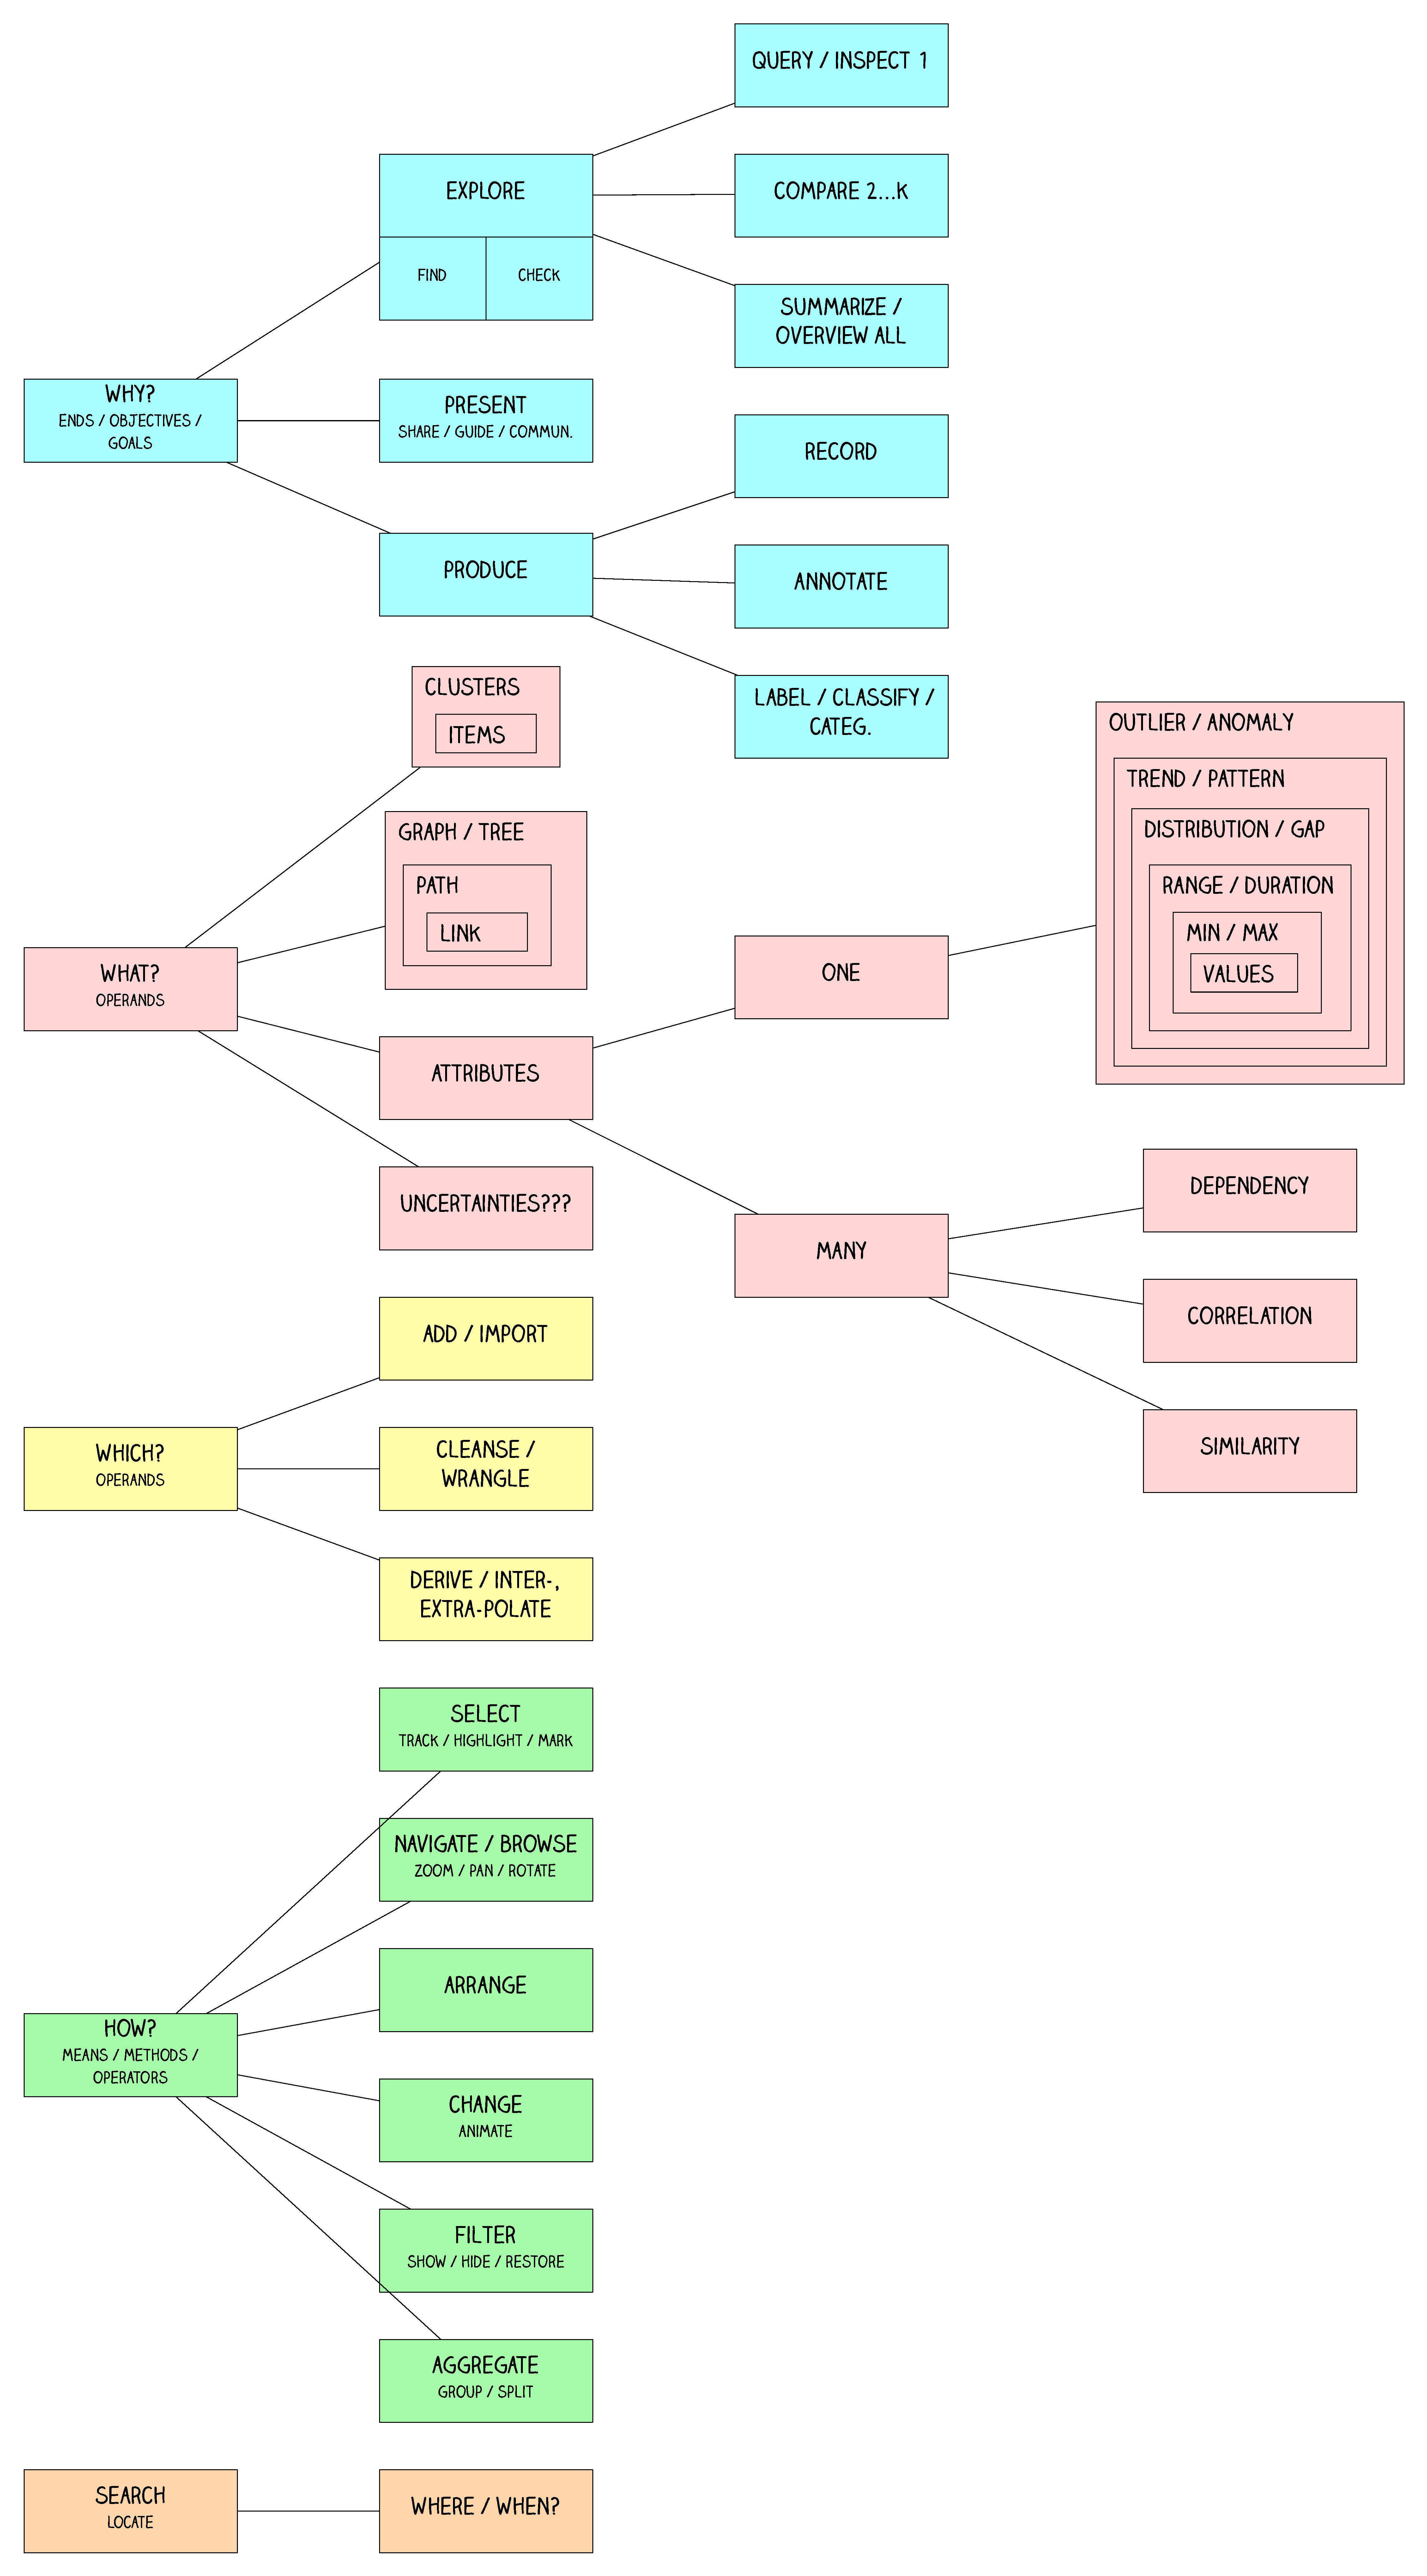
\includegraphics[width=0.75\textwidth]{figures/typology-12-11-30.pdf}
	\caption
	[
	    Our third classification.
	]
	{
	    {\bf November 30, 2012}: Our third classification, which introduced \textsl{why}, \textsl{how}, \textsl{what}, \textsl{which}, as a means to group terms, as well as a special case for {\tt search}.
	}
	\centering
	\label{app:typology:fig:12.11.30}
\end{figure}

%-|-|-|-|-|-|-|-|-|-|-|-|-|-|-|-|-|-|-|-|-|-|-|-|-|-|-|-|-|-|-|-|-|-|-|-|-

\bstart{November 2012 -- February 2013}
While we refined our classification, I continued to consult additional literature during this period, now venturing further from the core visualization literature to literature from the \ac{HCI}\index{human-computer interaction (HCI)}, information retrieval\index{information retrieval}, communications\index{communications}, and distribution cognition\index{distributed cognition} research communities.

\refstepcounter{papernumber} 
\begin{sloppypar}
\bstart{December 7, 2012\thepapernumber}
\bibentry{Liu2008}~\cite{Liu2008}. \end{sloppypar}

\begin{quotation}
    A discussion of distributed cognition\index{distributed cognition} theory in the context of visualization, distinguishing between {\it epistemic}\index{distributed cognition!epistemic actions} and {\it pragmatic} actions\index{distributed cognition!pragmatic actions}.
    Pragmatic actions\index{distributed cognition!pragmatic actions} are explicitly and consciously goal-directed, while epistemic actions\index{distributed cognition!epistemic actions} serve to coordinate actors' internal mental models with external representations of information.
    
    Information is propagated as a series of {\it representation states}, some are external within or between representations and artefacts, while some are internal to individuals (or shared between individuals).
    In the context of visualization, distributed cognition\index{distributed cognition} can help us to acknowledge both external and internal states of information, to capture the process of coupling, coordination, interaction\index{interaction} strategies for sensemaking\index{sensemaking} and analytical reasoning, the creation and evolution of external representations, and the role of interaction\index{interaction} in aiding understanding. 
    
    The authors state: ``{\it A science of interaction should not be just a taxonomy of interaction techniques or a framework of the abstracted task\index{task} procedures; it should be a scientific approach to understand how cognition emerges as a property of interaction between internal and external representations.}''
    
    Referred to in the meta-analysis of cognitive science theories by \citet{Pohl2012} (see above).
\end{quotation}

\bstart{December 9, 2012}
Prior to our fourth classification, we performed more brainstorming and diagramming such as in \autoref{app:typology:fig:12.12.09}.

%-|-|-|-|-|-|-|-|-|-|-|-|-|-|-|-|-|-|-|-|-|-|-|-|-|-|-|-|-|-|-|-|-|-|-|-|-

\begin{figure}
	\centering
	\includegraphics[width=\textwidth]{figures/typology-12-12-09.png}
	\caption
	[
	    Whiteboard and post-it diagramming prior to our fourth classification.
	]
	{
	    {\bf December 9, 2012}: Whiteboard and post-it diagramming prior to our fourth classification; we continued to iterate on a classification revolving around \textsl{why}, \textsl{how}, \textsl{what}, \textsl{which}, and {\tt search}.
	}
	\centering
	\label{app:typology:fig:12.12.09}
\end{figure}

%-|-|-|-|-|-|-|-|-|-|-|-|-|-|-|-|-|-|-|-|-|-|-|-|-|-|-|-|-|-|-|-|-|-|-|-|-

\refstepcounter{papernumber} 
\begin{sloppypar}
\bstart{December 17, 2012\thepapernumber}
\bibentry{Hollan2000}~\cite{Hollan2000}. \end{sloppypar}

\begin{quotation}
    An introduction to distributed cognition\index{distributed cognition} theory and the implications for \ac{HCI}\index{human-computer interaction (HCI)} research.
    Their suggested research framework involves studying {\it how people establish and coordinate structure within an environment}, {\it how coordination is maintained over time}, {\it how cognitive effort is offloaded to the environment when it is practical to do so}, achieving a better {\it conceptualization of what is going on and what ought to be done}, and {\it when and how cognitive load-balancing is achieved between human actors, the environment and its artefacts}.
    
    Referred to in the meta-analysis of cognitive science theories by \citet{Pohl2012} (see above).
\end{quotation}

\refstepcounter{papernumber} 
\begin{sloppypar}
\bstart{December 17, 2012\thepapernumber}
\bibentry{Kirsh1994}~\cite{Kirsh1994}. \end{sloppypar}

\begin{quotation}
    \begin{sloppypar}
    A distributed cognition\index{distributed cognition} paper that distinguishes {\it epistemic actions}\index{distributed cognition!epistemic actions} (gaining information about the problem at hand) from {\it pragmatic actions}\index{distributed cognition!pragmatic actions} (which support users toward their goals).
    {\it Epistemic actions}\index{distributed cognition!epistemic actions} are those that {\it make mental computation easier, faster, more reliable, less error prone, mediating intermediate results, reducing cognitive load, simplifying one's problem solving task\index{task}, reducing both space and time complexity}. 
    {\it Epistemic tasks}\index{distributed cognition!epistemic actions} are {\it memory- and time-saving actions, information gathering and exploratory actions}. 
    They are intended as {\it external checks or verifications to reduce the uncertainty of judgments}\index{uncertainty}.
    \end{sloppypar}
    
    Referred to in the meta-analysis of cognitive science theories by \citet{Pohl2012} (see above).
\end{quotation}

\refstepcounter{papernumber} 
\begin{sloppypar}
\bstart{December 18, 2012\thepapernumber}
\bibentry{Kirsh2006}~\cite{Kirsh2006}. \end{sloppypar}

\begin{quotation}
    A brief article that discusses the methodological and design implications of a distributed cognition\index{distributed cognition} framework for \ac{HCI}\index{human-computer interaction (HCI)}.
    
    Kirsh states: ``{\it Formalism-based abstractions on task\index{task} environments or task procedures are the major approaches for studying how people interact\index{interaction} with artefacts and other people, yet these are known to be flawed in making unreasonable assumptions about the predictability of human behaviours and characterizing the environment as a fixes set of choice points.}''

    This work was cited in our original submission but not in the  \autoref{ch:typology} or the published version of \citet{Brehmer2013}, as we opted for more comprehensive references to the distributed cognition\index{distributed cognition} literature, such as \citet{Hollan2000} and \citet{Kirsh1994}.
\end{quotation}

\bstart{December 19, 2012}
As we continued to iterate on our meta-analysis and classification efforts, we considered how to explicitly frame our project using the language of Tamara's Nested model~\cite{Munzner2009}\index{nested model (Munzner)}\footnote{This framing was documented in our second slide presentation, as explained in \autoref{app:typology:meta-analysis}.}.
We also added a distributed cognition\index{distributed cognition} framing to our meta-analysis of existing classifications and specifically the distinction between {\it pragmatic}\index{distributed cognition!pragmatic actions} and {\it epistemic}\index{distributed cognition!epistemic actions} actions.
We also began to group terms around nodes in our classifications, which would eventually lead to \autoref{typology:tab:rw:why} and \autoref{typology:tab:rw:how}.

\refstepcounter{papernumber} 
\begin{sloppypar}
\bstart{December 15 2012 -- January 3, 2013\thepapernumber}
\bibentry{Kuhn1962}~\cite{Kuhn1962}. \end{sloppypar}

\begin{quotation}
    Discusses how {\it normal science} is a puzzle-solving process governed by {\it paradigms} (abstractions shared by those within a specific discipline, describing what the puzzle looks like and what parts of the puzzle remain to be solved), which in turn influence a set of rules, by which the course of normal scientific experimentation, measurement, analysis, and theorizing proceed. 
    
    {\it Anomaly}, {\it invention}, and {\it discovery} are violations to the order of {\it normal science} and the expectations that a paradigm has provided.
    Exploration of the anomaly leads to a {\it paradigm shift}, and during this shift, disagreement about these discoveries leads to a state of crisis in which new theories emerge.
    
    Recommended by committee member Ron Rensink; we did not cite this work in \autoref{ch:typology} or \citet{Brehmer2013}, as Kuhn is referring to a much larger scope of processes encompassing in entire scientific discipline, whereas we focused on processed of individuals or groups as they use a certain class of tools and techniques.
\end{quotation}

\refstepcounter{papernumber} 
\begin{sloppypar}
\bstart{January 3--4, 2013\thepapernumber}
\bibentry{Case2008}~\cite{Case2008}. \end{sloppypar}

\begin{quotation}
    In a Chapter called ``{\it Models of information behaviour}'', Case surveys five models of {\it information seeking} intended to generalize over a wide population, considering various needs, individual differences, forms of media.
    Case places an emphasis on casual information seeking and non-work-related motivators.
    
    In a Chapter called ``{\it Theories, perspectives, paradigms}'', Case discusses the paradigms (with nods to \citet{Kuhn1962}) and theoretical perspectives relating to information behaviour.
    Case reviews five major theories and their sources relating to information seeking behaviour, emanating from psychology, sociology, communications, management and business, consumer research, economics, and linguistics. 
    Included among these theories is {\it sensemaking}\index{sensemaking} and {\it play theory}\index{play theory (Stephenson)} (see discussion of \citet{Stephenson1967} below).
    
    I became aware of this work via UBC InfoVis group member Jessica Dawson, who in early 2012 had completed a UBC Library and Information Studies graduate seminar course (LIBR 553 2011-12: {\it Understanding information users in diverse environments}); \citet{Case2008} was required reading for this course. 
    This work was cited in our original submission but not in the  \autoref{ch:typology} or the published version of \citet{Brehmer2013}, opting to cite original sources such as \citet{Toms2000} instead.
\end{quotation}

\refstepcounter{papernumber} 
\begin{sloppypar}
\bstart{January 7, 2013\thepapernumber}
\bibentry{Toms1999}~\cite{Toms1999}. \end{sloppypar}

\begin{quotation}
    Discusses {\it serendipity} and the motivation for open-ended exploration: ``{\it significant evidence exists to support the concept that people also acquire information that was never sought and about which the individual may have had no predisposition.}''
    
    Helps to account for casual information retrieval\index{information retrieval}: ``{\it "There was no need, no anomalous state of knowledge and no knowledge gap evident. This was simply an information gathering experience without expectations or predicted outcome novelty stimulated curiosity (and thus exploration).}''
    This work was cited in our original submission but not in the  \autoref{ch:typology} or the published version of \citet{Brehmer2013}, opting to cite the more comprehensive \citet{Toms2000} paper instead.
\end{quotation}

\refstepcounter{papernumber} 
\begin{sloppypar}
\bstart{January 8, 2013\thepapernumber}
\bibentry{Toms2000}~\cite{Toms2000}. \end{sloppypar}

\begin{quotation}
    Makes compelling or noteworthy assertions about the browsing behaviour of people who use information retrieval\index{information retrieval} tools, reporting on an experiment in which two groups of participants read related news articles, where one group was given a learning objective and another was not; the two groups' interactions\index{interaction} and usage of the articles varied.
    
    Toms remarks that the terms {\it browsing, navigating, exploring, way-finding, travelling, orienteering, foraging, grazing, wandering, surfing}, and {\it skimming} are often conflated. 
    {\it Browsing} relies on juxtapositions of content in time and space, presented within a context that stimulates a person; ``{\it browsing may be more like news reading, more in line with the play theory\index{play theory (Stephenson)} of \citet{Stephenson1967}. The success of browsing may be in the experience itself and not in the outcome.}''
    
    This paper was also part of the syllabus for LIBR 553 2011-12: {\it Understanding information users in diverse environments}, along with \citet{Case2008}.
\end{quotation}

\bstart{January 9, 2013}
Our fourth classification is represented in \autoref{app:typology:fig:13.01.09}.
By this point, we consolidated {\it search} and {\it why} and we established a stronger associated between {\it which} and {\it what}.
We also began to use the terms {\it  epistemic}\index{distributed cognition!epistemic actions} and {\it pragmatic}\index{distributed cognition!pragmatic actions}, which we borrowed from the distributed cognition\index{distributed cognition} literature\footnote{We documented these developments in our third slide presentation, as explained in \autoref{app:typology:meta-analysis}.}.

%-|-|-|-|-|-|-|-|-|-|-|-|-|-|-|-|-|-|-|-|-|-|-|-|-|-|-|-|-|-|-|-|-|-|-|-|-

\begin{figure}
	\centering
	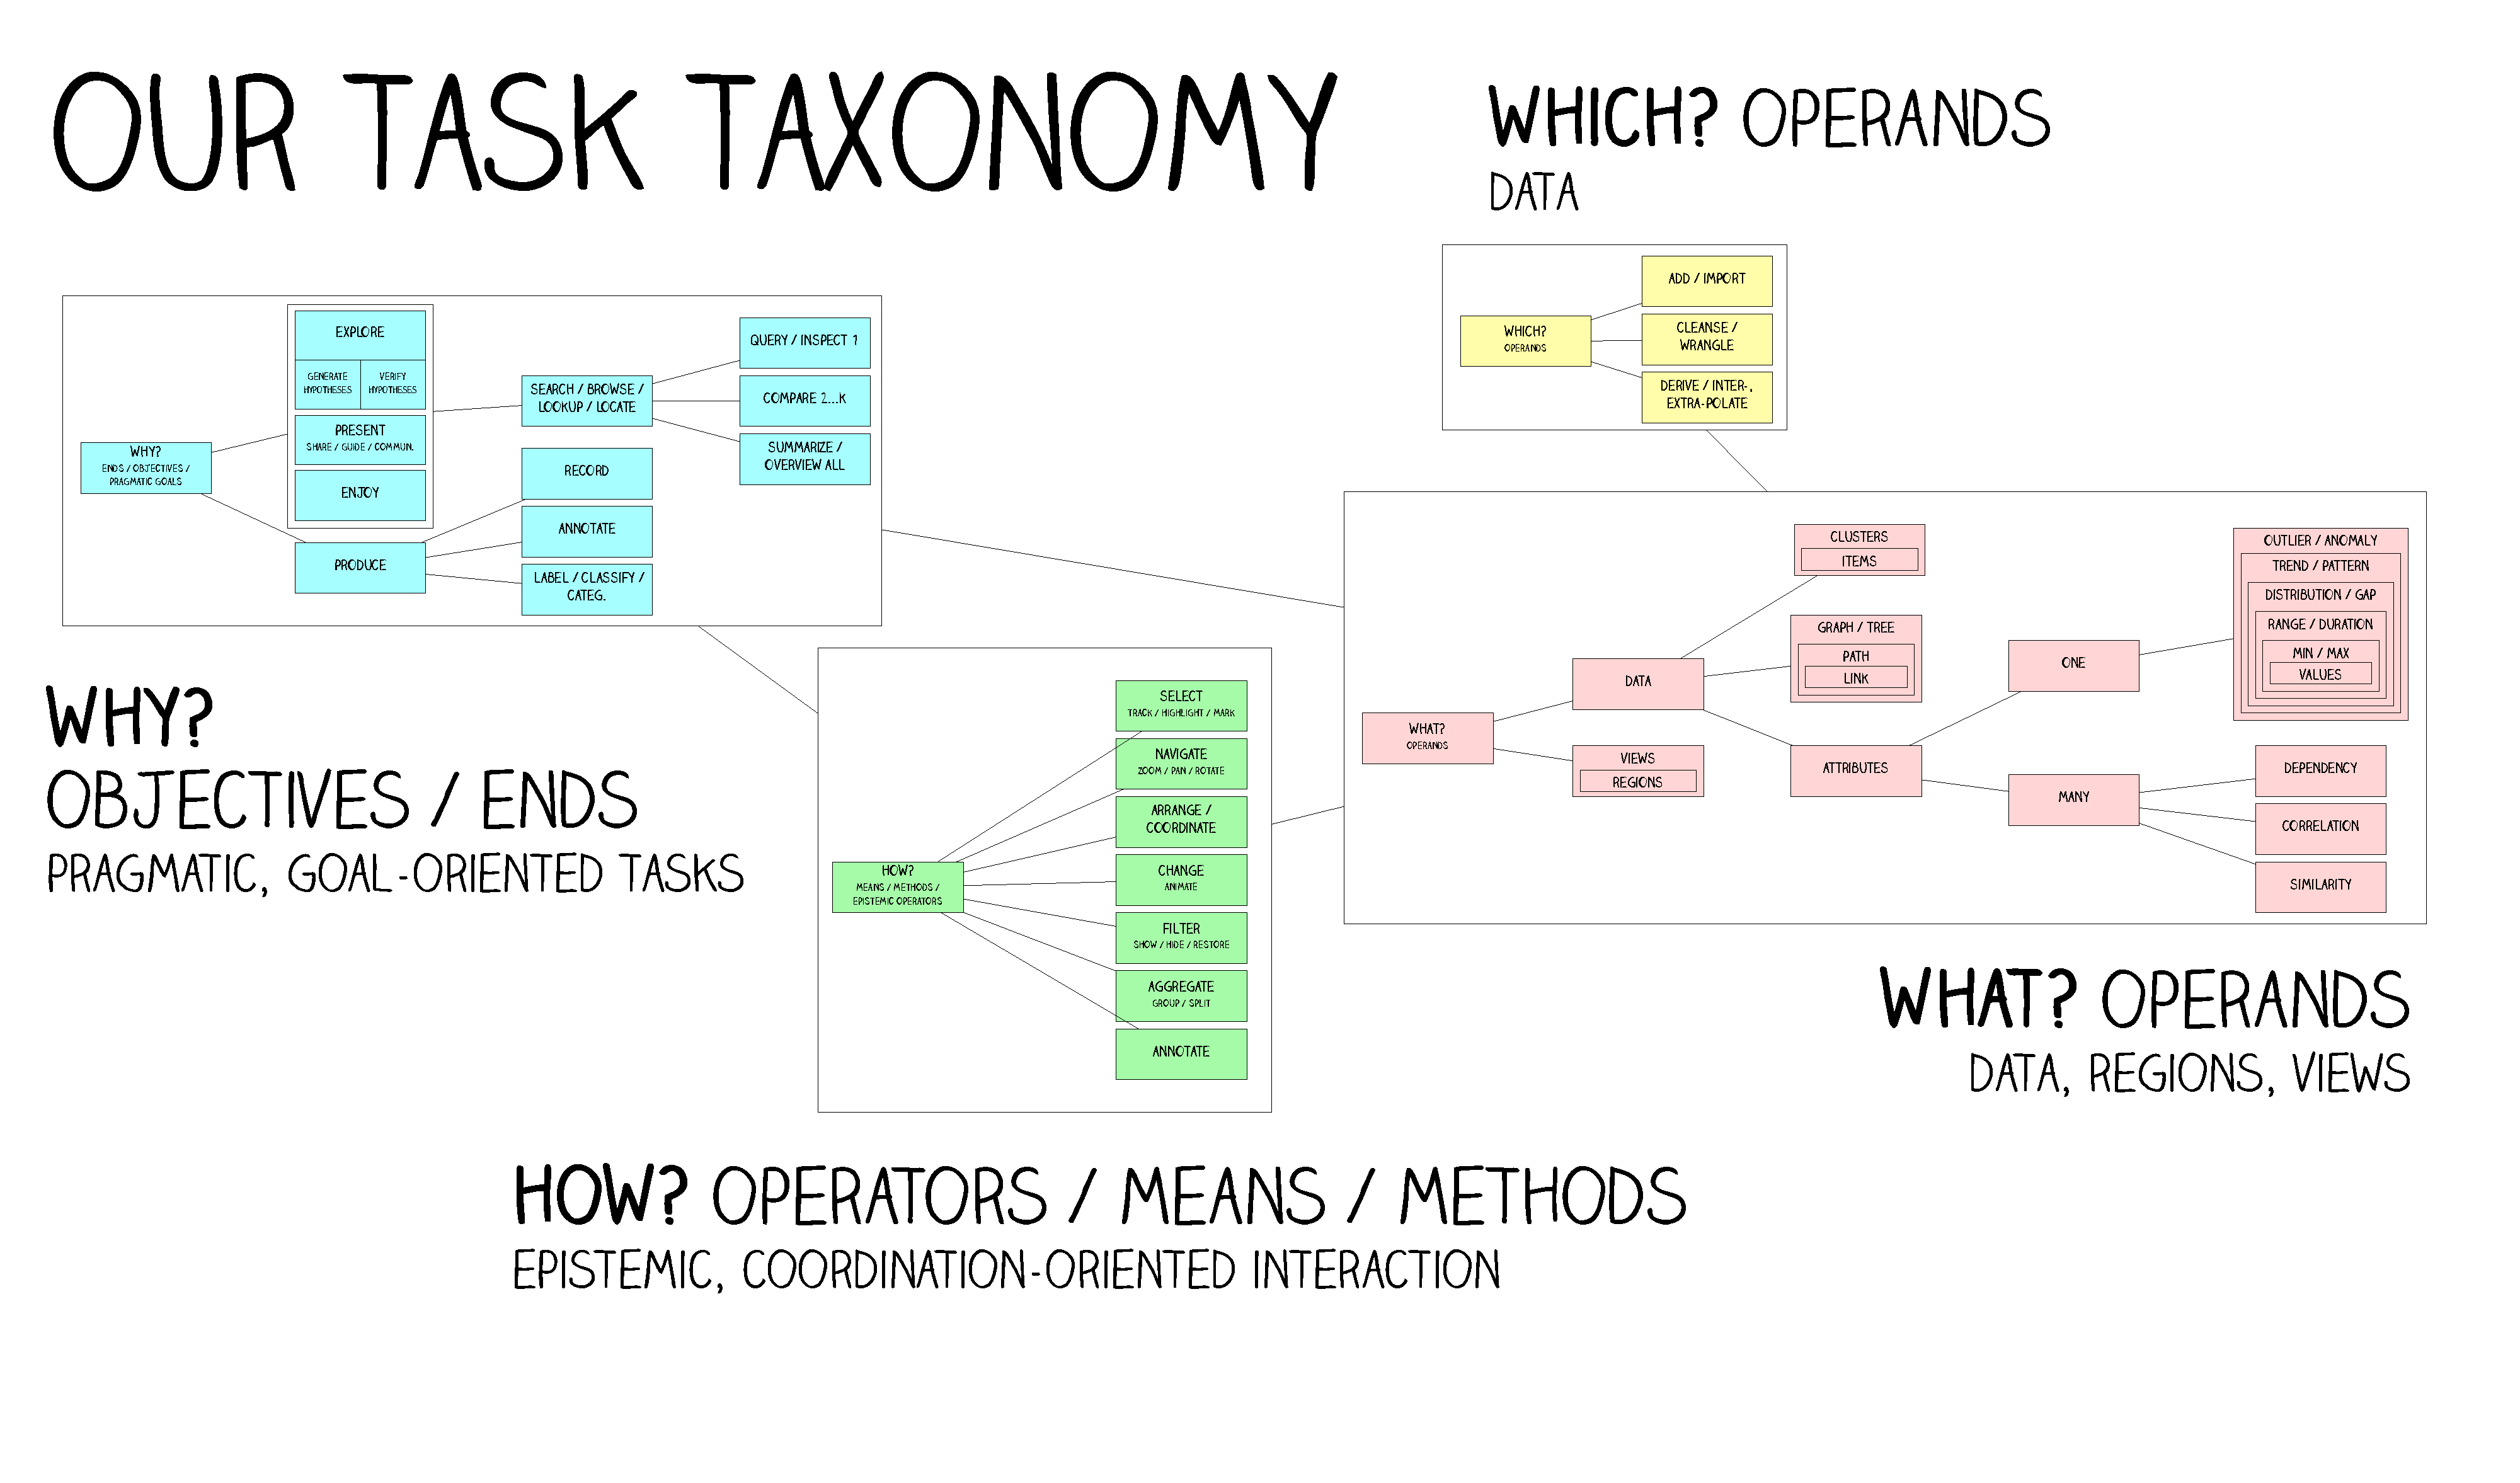
\includegraphics[width=\textwidth]{figures/typology-13-01-09.pdf}
	\caption
	[
	    Our fourth classification.
	]
	{
	    {\bf January 9, 2013}: Our fourth classification, where \textsl{why} corresponds to objectives / ends, \textsl{how} corresponds to operators / means / methods, while \textsl{what} and \textsl{which} correspond to operands. Note that we begin to use the terms {\it epistemic} and {\it pragmatic}, which we borrow from the distributed cognition literature.
	}
	\centering
	\label{app:typology:fig:13.01.09}
\end{figure}

%-|-|-|-|-|-|-|-|-|-|-|-|-|-|-|-|-|-|-|-|-|-|-|-|-|-|-|-|-|-|-|-|-|-|-|-|-

\refstepcounter{papernumber} 
\begin{sloppypar}
\bstart{January 11, 2013\thepapernumber}
\bibentry{Norman1988}~\cite{Norman1988}. \end{sloppypar}

\begin{quotation}
    Norman's {\it Stages of Action} model has seven stages and two gulfs: {\it stage 1: forming the goal}, the {\it gulf of execution}, {\it stage 2: forming the intention}, {\it 3: specifying the action}, {\it 4: executing the action}, the {\it gulf of evaluation}, {\it stage 5: perceiving the state of the system}, {\it 6: interpreting the state of the system}, and {\it 7: evaluating the outcome}. 

    \begin{sloppypar}
    Norman's model\index{stages of action (Norman)} and its influence on Roth's {\it objective-operand-operator} meta-analysis~\cite{Roth2012a} of previous classifications helped shape the {\it why-what-how} organization of our typology.
    \end{sloppypar}
    
    \citet{Lam2008} (discussed above) extended Norman's model in the context of visualization with a {\it gulf of goal formation}, relevant whenever a person articulates their own questions pertaining to visualized data.
\end{quotation}

\refstepcounter{papernumber} 
\begin{sloppypar}
\bstart{January 14, 2013\thepapernumber}
\bibentry{Roth2012}~\cite{Roth2012}. \end{sloppypar}

\begin{quotation}
    \begin{sloppypar}
    Contributes a datatype specific classification of interaction\index{interaction} primitives relating to cartographic\index{cartography} data based on Norman's {\it Stages of Action} model, distinguishing between {\it goals} (or {\it meta-objectives}: {\it procure, predict, prescribe}), {\it objectives} ({\it identify, compare, rank, associate, delineate}), {\it operators}, and {\it operands}.
    \end{sloppypar}
    
    Among Roth's list of {\it operators} are {\it work operators} ({\it re-express, arrange, sequence, re-symbolize, overlay, re-project, pan, zoom, filter, search, retrieve, calculate}) and {\it enabling operators} ({\it import, export, save, edit, annotate}).
    
    With respect to {\it operands}, Roth distinguishes between the {\it search target} ({\it in space alone, in space-in-time, an attribute-in-space}) and {\it search level} ({\it elementary, general}).
    
    Roth arrived at this classification via a series of card-sorting exercises on {\it objectives} and {\it operators} and 15 cartographic\index{cartography} interface designer/developer participants. 
    His rationale for this method: ``{\it One limitation of extant taxonomies contributing to their lack of general adoption is that the majority of these taxonomies are not empirically derived, instead relying on secondary sources or personal experience.}''
    Roth noted a high degree of variability in responses across the {\it objectives}, as there appeared to be some confusion stemming from different {\it operands}.
    
    A longer version of this short workshop paper appeared as \citet{Roth2013} at IEEE InfoVis 2013 (see below).
\end{quotation}

\refstepcounter{papernumber} 
\begin{sloppypar}
\bstart{January 14, 2013\thepapernumber}
\bibentry{Pike2009}~\cite{Pike2009}. \end{sloppypar}

\begin{quotation}
    A survey and research agenda highlighting challenges in interaction\index{interaction} within the visual analytics\index{visual analytics} community.
    Prior to addressing the research agenda, they provide a domain- and datatype-agnostic classification that spans low-level\index{task!low-level tasks} and high-level tasks\index{task!high-level tasks}, consolidating prior work from the same group by \citet{Amar2004}, \citet{Amar2005}, and \citet{Yi2007}.
    
    The authors state that despite many prior classifications, they see a need to understand a relationship between task/interaction\index{interaction} components and modes of inquiry: {\it abduction} (constructing hypotheses), {\it deduction} (refuting prior hypotheses), {\it induction} (verification, ranking alternative hypotheses, identifying the best explanation).
    
    Among {\it user goals} or {\it tasks}, they distinguish between {\it high-level} ({\it explore, analyze, browse, assimilate, triage, show understand, compare}) and {\it low-level} (from \citet{Amar2005}: {\it retrieve value, filter, sort, compute derived value, find extremum, correlate, determine range, cluster, characterize distribution, find anomalies}).
    
    The authors distinguish between {\it techniques} and {\it intents}, in that the former should never be considered as an ends in itself, but    ``{\it a means to support the user's information understanding}''.
    
    When characterizing {\it interactive visualization}, the authors distinguish between {\it high-level representation intents} ({\it depict, differentiate, identify, show outliers, compare}),  {\it high-level interaction intents} (from \citet{Yi2007}: {\it select, explore, reconfigure, encode\index{visual encoding}, abstract, elaborate, filter, connect}), {\it low-level representation techniques} ({\it charts, graphs, networks\index{network data}, treemaps, parallel coordinates}) and {\it low-level interaction techniques} ({\it selection, brushing\index{view coordination!brushing across views}, dynamic query, pan, zoom}).
\end{quotation}

\refstepcounter{papernumber} 
\begin{sloppypar}
\bstart{January 14, 2013\thepapernumber}
\bibentry{Klein2006a}~\cite{Klein2006a}. \end{sloppypar}

\begin{quotation}
    Discusses {\it sensemaking}\index{sensemaking}, misconceptions about {\it sensemaking}\index{sensemaking}, and its distinguishing features.
    {\it Sensemaking}\index{sensemaking} is about {\it understanding connections, anticipating trajectories, making predictions}, and {\it acting effectively (\ie making decisions)}; it is highly iterative and has no clear start and end points.

    We did not cite this work in \autoref{ch:typology} or \citet{Brehmer2013}, as we opted to cite \citet{Klein2006} instead (discussed below), which contributes a classification.
\end{quotation}

\refstepcounter{papernumber} 
\begin{sloppypar}
\bstart{January 14, 2013\thepapernumber}
\bibentry{Klein2006}~\cite{Klein2006}. \end{sloppypar}

\begin{quotation}
    Contributes a high-level classification / model\index{task!high-level tasks}: the {\it data-frame} model of {\it sensemaking}\index{sensemaking}, which involves a {\it elaboration cycle} and a {\it reframing cycle}.
    
    The {\it elaboration cycle} involves {\it recognizing and constructing a frame}, {\it managing attention within a frame, defining, connecting}, and {\it filtering data}, {\it elaborating a frame} ({\it adding and filling slots, seeking and inferring new data and relationships, discarding data}), {\it questioning a frame} ({\it tracking anomalies, detecting inconsistencies, judging plausibility, gauging data quality}), and {\it preserving a frame}.
    
   \begin{sloppypar}
   The {\it reframing cycle} involves {\it comparing} and {\it seeking new frames}.
   \end{sloppypar} 
    
    The relationship between a data and a {\it frame} is one of {\it assimilating} data into a frame and {\it accommodating} frames via {\it questioning, rejecting}, and {\it comparing} of alternative frames.
    {\it Sensemaking}\index{sensemaking} is a process by which multiple {\it frames} or hypotheses are considered.
\end{quotation}

\refstepcounter{papernumber} 
\begin{sloppypar}
\bstart{January 15, 2013\thepapernumber}
\bibentry{Lee2012}~\cite{Lee2012}. \end{sloppypar}

\begin{quotation}
    A discussion of post-\ac{WIMP} interfaces and the prospects for visualization tools and techniques. 
    With respect to interaction\index{interaction} in general, the authors characterize how an interaction\index{interaction} begins with an {\it intent}, followed by an {\it action}, which triggers some {\it feedback} from the system and in return a {\it reaction} to that feedback.
    
    They argue: ``{\it InfoVis interaction taxonomies consider the system reaction or the resulting functionality part of the interaction timeline largely discuss interaction from the viewpoint of interaction tasks\index{task} to be performed with and on the data, or from interaction techniques that can be performed on the data or its visual representation. We take a human-centric approach instead and do not specify data or tasks}.''
    
    The authors correctly point out that many classifications of interaction\index{interaction} techniques for data exploration ``{\it are often mixed and discussed interchangeably with those related to an analyst's tasks with a visualization}.''
\end{quotation}

\bstart{January 16, 2013}
We continued to refine our meta-analysis of existing classifications, as represented in \autoref{app:typology:fig:cross-cuts}.
These cross-cutting dimensions refer to terms defined by \citet{Chi1998} ({\it temporal} vs. {\it atemporal}), \citet{Roth2012} ({\it objective}, {\it operator}, and {\it operand}, which is in turn influenced by \citet{Norman1988}'s {\it Stages of Action} model), \citet{Chuah1996} ({\it semantic}, {\it syntactic}, and {\it lexical}, \citet{Beaudouin-Lafon2004} ({\it descriptive}, {\it evaluative}, and {\it generative}), and \citet{Kirsh1994} ({\it pragmatic}\index{distributed cognition!pragmatic actions} and {\it epistemic}\index{distributed cognition!epistemic actions}).

\bstart{January 16, 2013}
I gave a pre-paper talk\footnote{For most papers written by members of the UBC InfoVis group, the lead author will present the paper to the group before it is written in the style of a conference presentation as a means to get feedback on the framing and contributions of the work; for more information, see \url{http://people.cs.ubc.ca/~tmm/policy.txt}.} about this project to the UBC InfoVis group, entitled {\it ``Mid-level Task Abstractions for Visualization Design and Evaluation''}\footnote{This was pre-paper talk was our fourth slide presentation, as explained in \autoref{app:typology:meta-analysis}.}.
This talk summarized our meta-analysis and our proposed classification shown in \autoref{app:typology:fig:13.01.09}.

\begin{sloppypar}
The group found our work to be compelling, however there was some confusion regarding the vocabulary that we used (\eg ``{\tt produce}''\index{{\tt produce}} vs. ``{\tt present}''\index{{\tt present}} and ``{\tt explore}''\index{{\tt explore}} vs. ``{\tt enjoy}''\index{{\tt enjoy}}), and whether a consideration of {\it who} was warranted alongside {\it why}, {\it what}, {\it how}, and {\it which}. 
They asked whether our scope accounted for even higher levels of abstract tasks, such as {\it understanding the past}, {\it decision making in the present}, and {\it predicting the future}.
They asked for more concrete examples to explain aspects of our classification.
There was also a question as to whether {\it which} was necessary and if it could be subsumed into the questions of {\it how} and/or {\it what}.
Some were confused about of the dimensions of our meta-analysis, particularly the {\it semantic}, {\it syntactic}, and {\it lexical} dimensions inspired by \citet{Chuah1996}.
The question of supporting evidence for our classification and our methodology also arose, indicating that we would need to thoroughly explain these aspects in subsequent presentations and in our eventual paper.
Finally, there was the question of how to validate our classification, which was not something we had planned to address in the paper; we planned to treat our classification as a proposal, and that validation would follow in subsequent projects over time.
\end{sloppypar}

%-|-|-|-|-|-|-|-|-|-|-|-|-|-|-|-|-|-|-|-|-|-|-|-|-|-|-|-|-|-|-|-|-|-|-|-|-

\begin{figure}
	\centering
	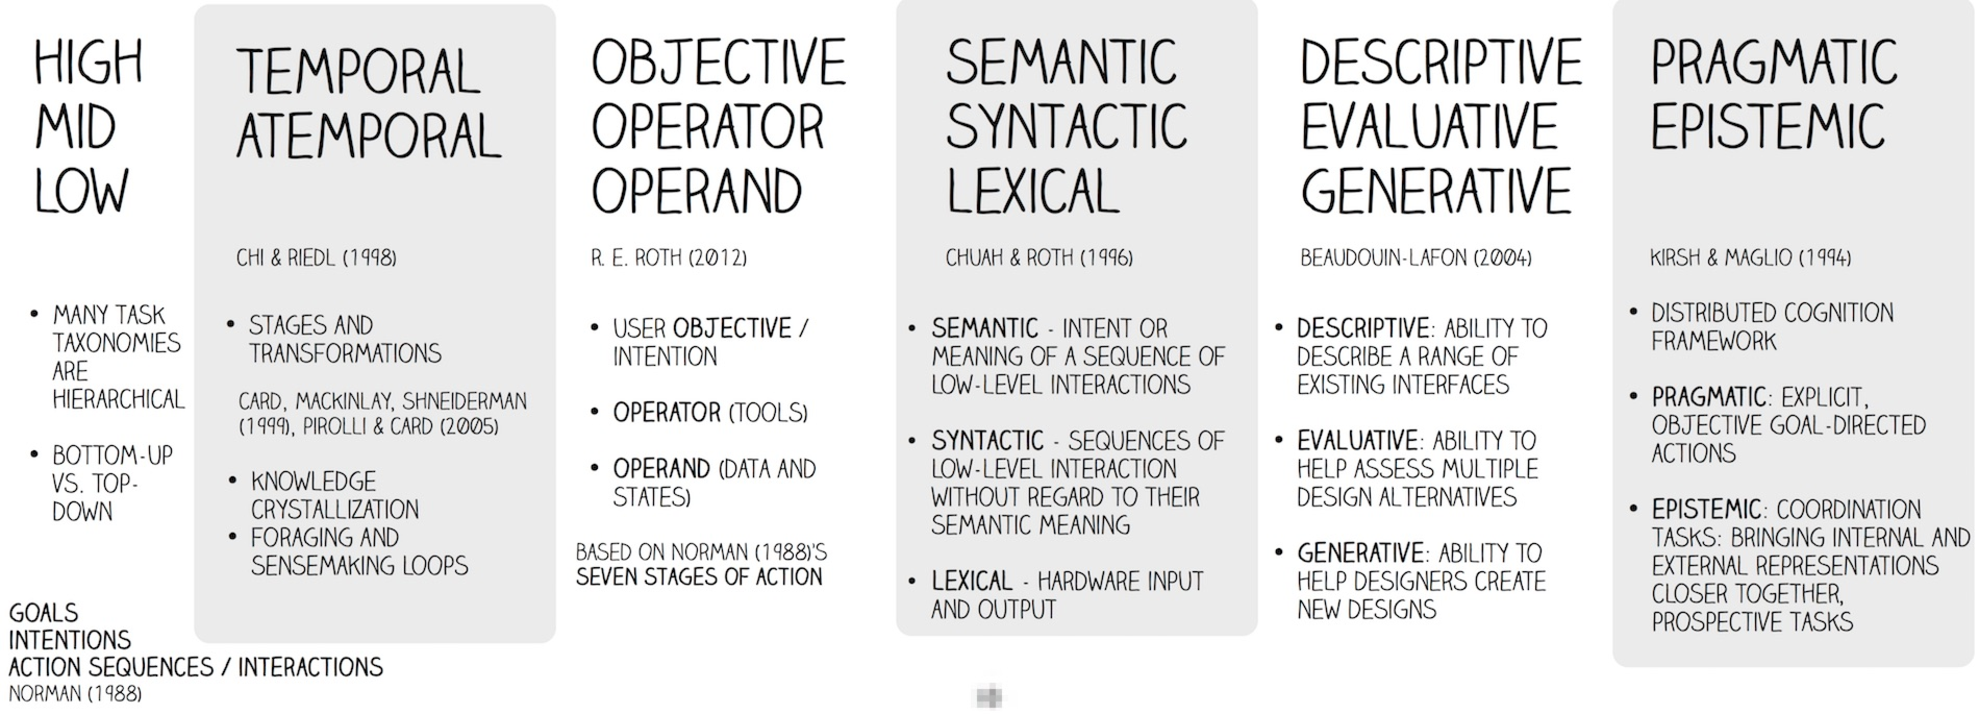
\includegraphics[width=\textwidth]{figures/typology-cross-cuts.pdf}
	\caption
	[
	    Cross-cutting dimensions of previous classifications or frameworks.
	]
	{
	    {\bf January 16, 2013}: Cross-cutting dimensions of previous classifications with dimensions using terms defined by \citet{Chi1998}, \citet{Roth2012} (which is in turn influenced by \citet{Norman1988}'s {\it Stages of Action} model), \citet{Chuah1996}, \citet{Beaudouin-Lafon2004}, and \citet{Kirsh1994}.
	}
	\centering
	\label{app:typology:fig:cross-cuts}
\end{figure}

%-|-|-|-|-|-|-|-|-|-|-|-|-|-|-|-|-|-|-|-|-|-|-|-|-|-|-|-|-|-|-|-|-|-|-|-|-

\bstart{January 16 -- February 2, 2013}
We consolidated the feedback we received in response to our pre-paper talk and refined our ideas and intended contributions over the next two weeks, and in this time we generated three additional iterations of slide presentations, as explained in \autoref{app:typology:meta-analysis}.
We also used this period to clarify our scope: we were not proposing an interaction\index{interaction} taxonomy, nor were we proposing a temporal pipeline model, and we certainly were not planning to enumerate or classify visual encoding\index{visual encoding} choices. 
With respect to {\it what}, we realized that we needed to distinguish {\it data} and {\it views}.
Finally, we realized that too much of our framing was contingent upon a deep familiarity with previous work from our group, namely Tamara's Nested Model~\cite{Munzner2009}\index{nested model (Munzner)}.

\refstepcounter{papernumber} 
\begin{sloppypar}
\bstart{January 25, 2013\thepapernumber}
\bibentry{Buxton1986}~\cite{Buxton1986}. \end{sloppypar}

\begin{quotation}
    Discusses interaction techniques designed around chunking single actions into compound actions as a means to facilitate the development of expert skills.
    
    Recommended by co-advisor Joanna McGrenere in response to our pre-paper talk and our discussion of ``nested tasks''. 
    We did not cite this work in \autoref{ch:typology} or \citet{Brehmer2013}, as we recast nested tasks as sequences of interdependent tasks\index{task!task sequence}.
\end{quotation}

\refstepcounter{papernumber} 
\begin{sloppypar}
\bstart{January 28, 2013\thepapernumber}
\bibentry{Kosara2013}~\cite{Kosara2013}. \end{sloppypar}

\begin{quotation}
    Discusses the role and prospects of visualization in presentation and storytelling\index{storytelling}.
    The authors discuss presentation in collaborative and pedagogical contexts, and the way in which a presentation is given may vary according to the size of the audience, whether the presentation is live or pre-recorded, and whether the audience is co-located with the presenter.
\end{quotation}

\refstepcounter{papernumber} 
\begin{sloppypar}
\bstart{February 1, 2013\thepapernumber}
\bibentry{Card1997}~\cite{Card1997}. \end{sloppypar}

\begin{quotation}
    Presents a grammar or language for describing a mapping between abstract data types and common (visual encodings)\index{visual encoding}, distinguishing between data and {\it derived} or {\it transformed} data.
    Transformations can include {\it filtering, sorting, \ac{MDS}, interactive input}, and other functions.
    
    This work was cited in our original submission but not in the  \autoref{ch:typology} or the published version of \citet{Brehmer2013}, as the authors do not explicitly discuss tasks\index{task} but focus on the visual encoding\index{visual encoding} design space, which we did not address.
\end{quotation}

\refstepcounter{papernumber} 
\begin{sloppypar}
\bstart{February 1, 2013\thepapernumber}
\bibentry{Spence2007}~\cite{Spence2007}. \end{sloppypar}

\begin{quotation}
    Contributes a classification that distinguished between {\it interaction modes} ({\it continuous, stepped, passive}, and {\it composite interaction}) and {\it interaction spaces} ({\it continuous, discrete}).

    Regarding intention, Spence says that a person could be {\it learning} ({\it exploring}), {\it seeking} ({\it finding}), or {\it interacting in an opportunistic or involuntary manner}. 
    {\it Browsing} ({\it perusal}) can occur in any of these situations, and Spence refers to the perception and interpretation of content, including navigational cues.
    
    Regarding interaction\index{interaction}, Spence invokes \citet{Norman1988} and the {\it Stages of Action} model.
    He distinguishes some interaction as being related to {\it navigation}, {\it sensitivity}, {\it making dynamic queries}, and {\it evaluating residue or information scent}.
\end{quotation}

\refstepcounter{papernumber} 
\begin{sloppypar}
\bstart{February 1, 2013\thepapernumber}
\bibentry{Friel2001}~\cite{Friel2001}. \end{sloppypar}

\begin{quotation}
    Makes compelling or noteworthy assertions about the behaviour of people who use graphs, distinguishing two high-level uses of graphs: {\it translation} ({\it locating}) and {\it interpretation} / {\it integrating} (involving {\it re-arranging, sorting, filtering}, and its {\it generative extensions interpolation} and {\it extrapolation}).
    
    Discusses analogous concepts in the comprehension of text, discerning between {\it inference, application, synthesis}, and {\it evaluation}, as well as {\it identifying gaps, contradictions, incongruities, anomalies}, and {\it ambiguities}.
    
    Included in the meta-analysis of graph comprehension theories by \citet{Pohl2012}, discussed above.
\end{quotation}

\refstepcounter{papernumber} 
\begin{sloppypar}
\bstart{February 1, 2013\thepapernumber}
\bibentry{Wilkinson2005}~\cite{Wilkinson2005}. \end{sloppypar}

\begin{quotation}
    Makes compelling or noteworthy assertions about the behaviour of people who use visualization tools or techniques, distinguishing between {\it building graphics} and {\it exploring interactive graphics}; the latter comprising of {\it filtering} {\it navigating} ({\it zooming, panning, lens}), {\it manipulating} ({\it node dragging, categorical reordering}), {\it brushing and linking}\index{view coordination!brushing across views}, {\it animating}\index{view coordination!animated transitions}, {\it rotating}, and {\it transforming}.
    
    \begin{sloppypar}
    Wilkinson also comments on the value of classification: ``{\it Classification for its own sake, however, is as unproductive in design as it is in science. In design, objects are only as useful as the system they support. And the test of a design is its ability to handle scenarios that include surprises, exceptions, and strategic reversals. [Classifications] may be useful for developing interfaces but contributes nothing to a deeper understanding of graphs. Customary usage and standards can blind us to the diversity of the graphics domain; a formal system can liberate us from conventional restrictions.}''
    \end{sloppypar}
    
    Presents a formal grammar for specifying graphics.
    This grammar is object-oriented, comprised of {\it sets, relations, functions, graphs, compositions, transformations, algebras, variables, varsets, frames}. 
    It describes how to {\it create variables, apply algebra, apply scales, compute statistics, construct geometries, apply coordinates}, and {\it compute aesthetics}.
\end{quotation}

\refstepcounter{papernumber} 
\begin{sloppypar}
\bstart{February 7, 2013\thepapernumber}
\bibentry{Bederson2003}~\cite{Bederson2003}. \end{sloppypar}

\begin{quotation}
    Discusses the purpose of theories for guiding visualization design and the {\it descriptive, explanatory, predictive, prescriptive}, and {\it generative} power of theories.
\end{quotation}

\refstepcounter{papernumber} 
\begin{sloppypar}
\bstart{February 7, 2013\thepapernumber}
\bibentry{Tweedie1997}~\cite{Tweedie1997}. \end{sloppypar}

\begin{quotation}
    \begin{sloppypar}
    Contributes a low-level classification\index{task!low-level tasks} of {\it interaction types} ({\it manual, mechanized, instructable, steerable, and automatic}) as well as the {\it directness} of interaction\index{interaction} ({\it direct} and {\it indirect manipulation}).
    \end{sloppypar}
    
    Describes three different levels of questions regarding data ({\it objects} and {\it attributes}): a single item, a set of items, or the whole set.
    
    Tweedie highlights {\it input} and {\it output} relations, as ``{\it this provides an externalization of the current state of the interaction}'. which is important if a person is to engage in a dialogue with a tool.
\end{quotation}

\bstart{February 7, 2013}
Our fifth classification is represented in \autoref{app:typology:fig:13.02.13}.
Based on the discussion that followed the pre-paper talk, we consolidated {\it which} with {\it how} and established a mid-level classification within {\it how}, distinguishing between {\tt encoding}\index{visual encoding} data elements, {\tt manipulating} elements, and {\tt introducing} elements.
The terms previously associated with {\it which} largely referred to {\tt introducing} elements, and thus were placed here.

%-|-|-|-|-|-|-|-|-|-|-|-|-|-|-|-|-|-|-|-|-|-|-|-|-|-|-|-|-|-|-|-|-|-|-|-|-

\begin{figure}
	\centering
	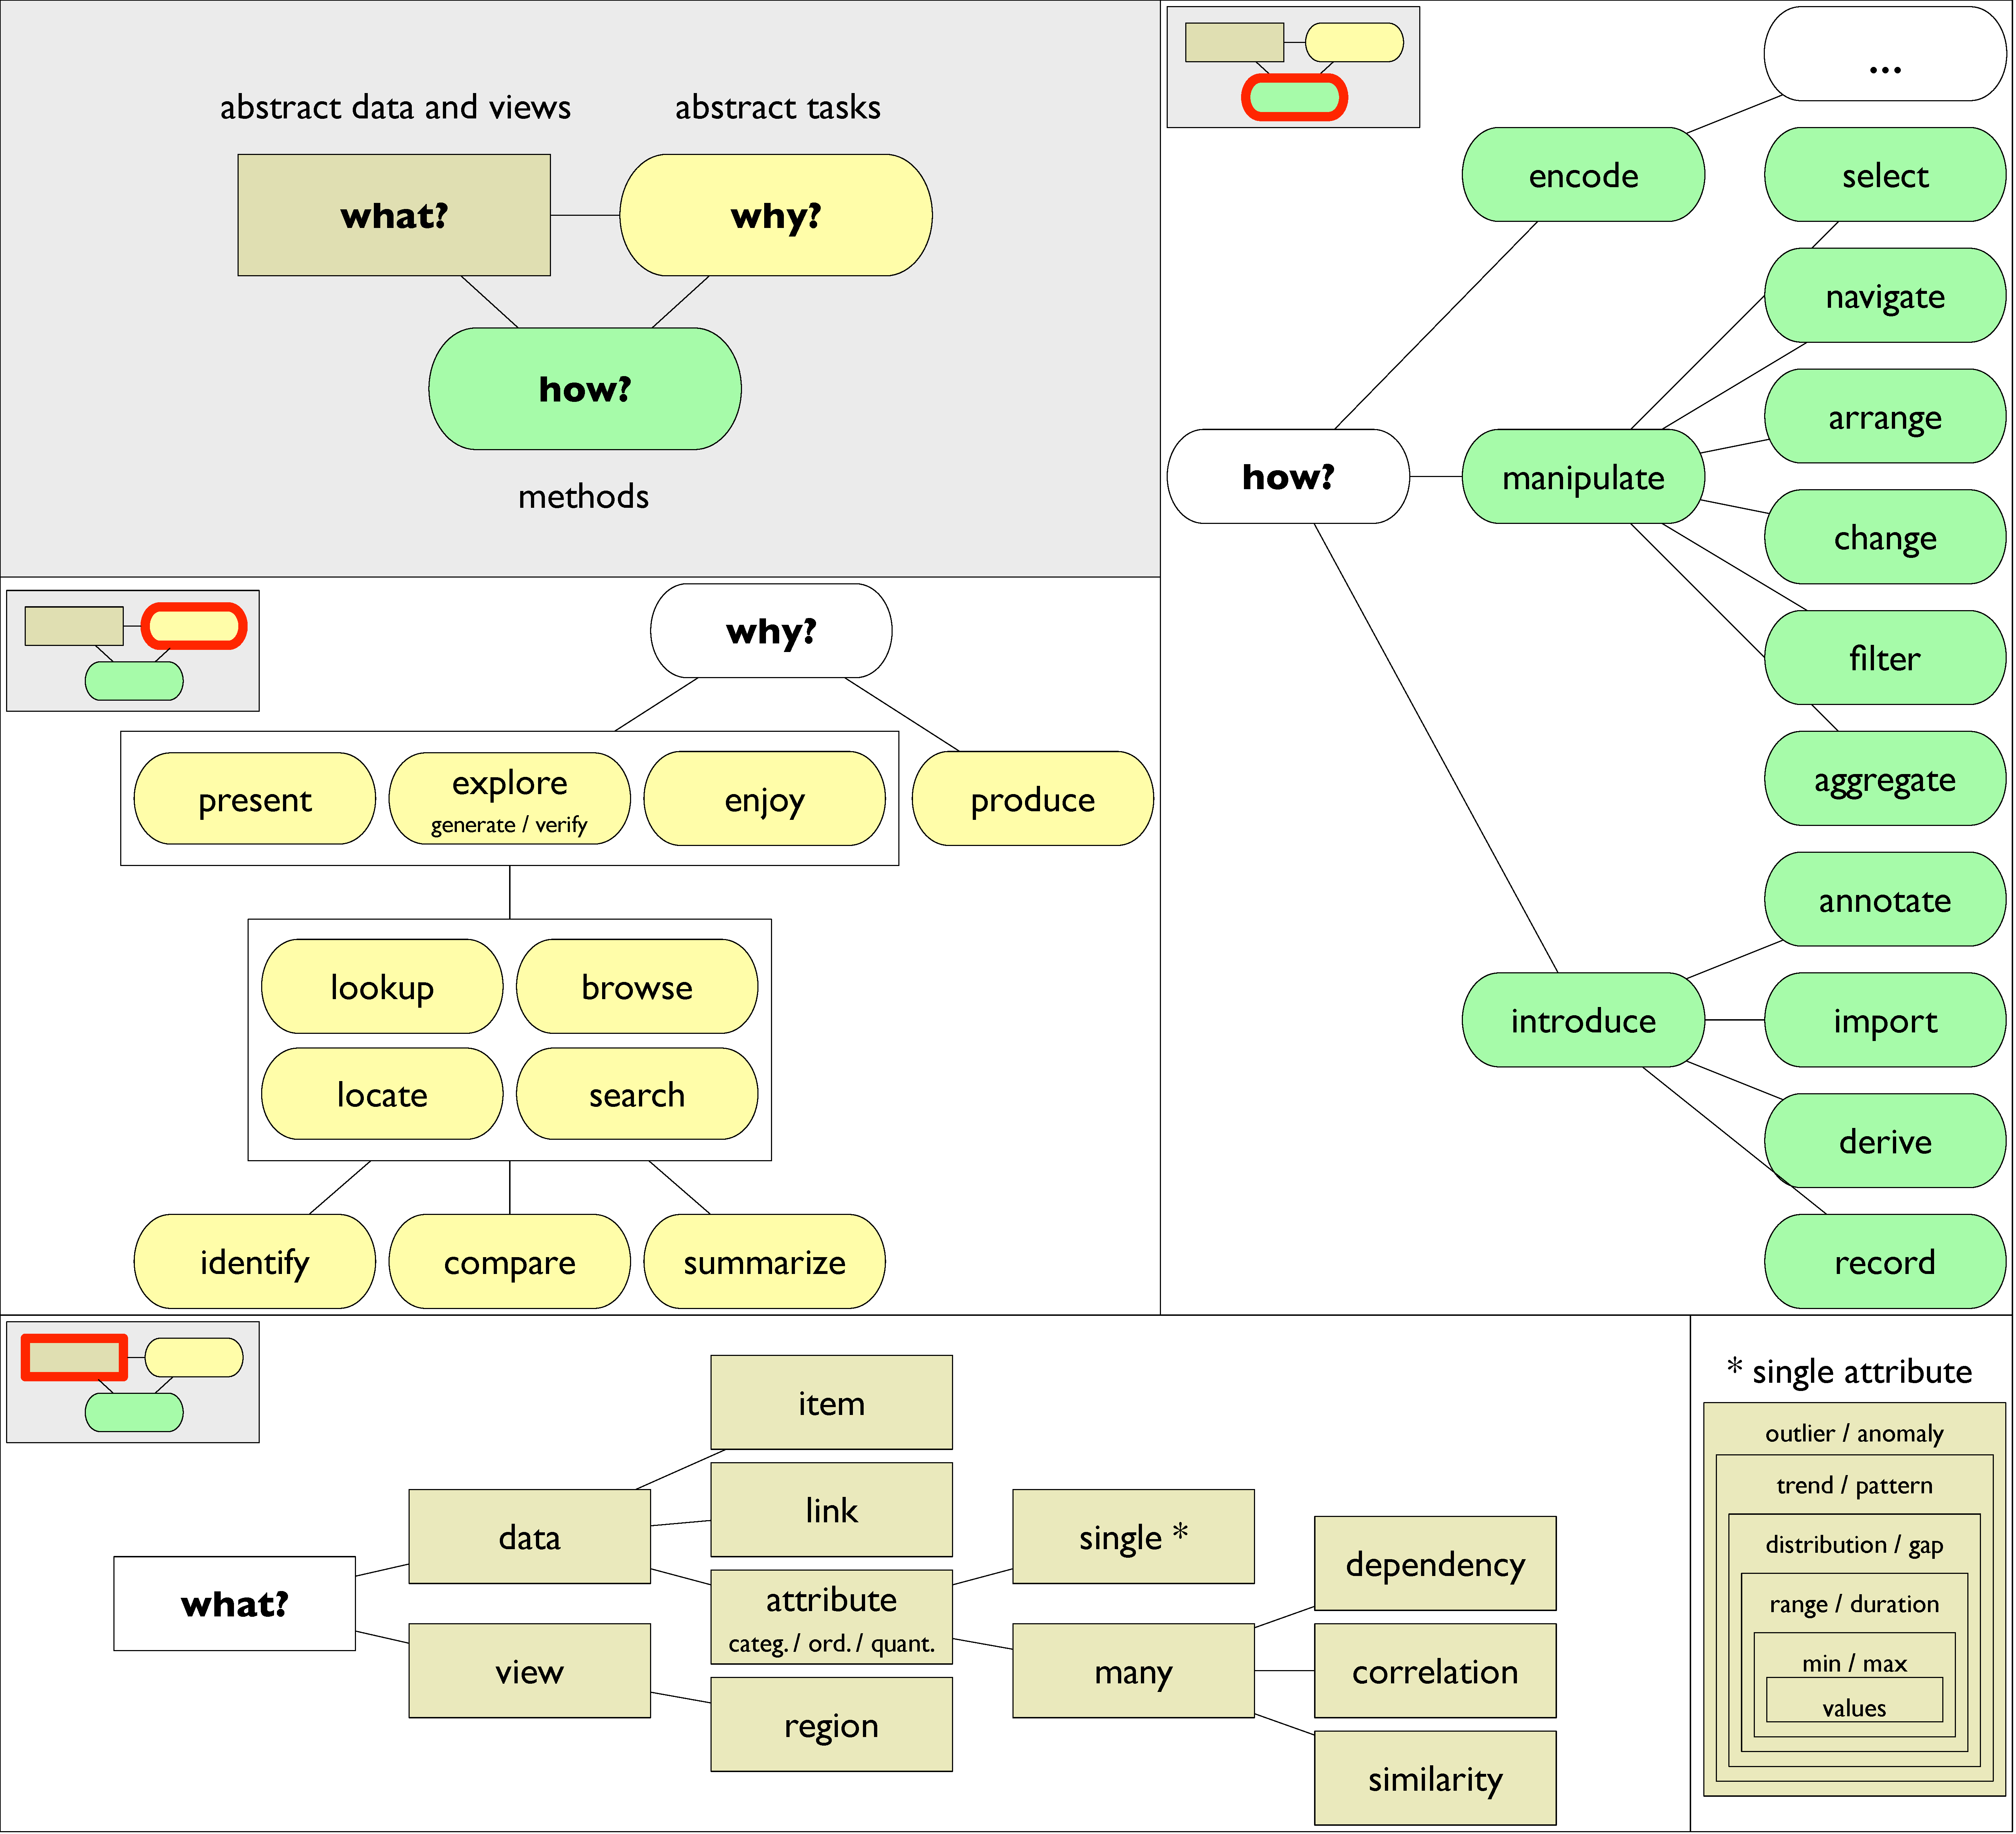
\includegraphics[width=0.975\textwidth]{figures/typology-13-02-13.pdf}
	\caption
	[
	    Our fifth classification.
	]
	{
	    {\bf February 13, 2013}: Our fifth classification, where \textsl{why} corresponds to abstract tasks, \textsl{how} corresponds to methods, and \textsl{what} corresponds to abstract data and views; the colours now correspond to Munzner's nested model~\cite{Munzner2009}.
	}
	\centering
	\label{app:typology:fig:13.02.13}
\end{figure}

%-|-|-|-|-|-|-|-|-|-|-|-|-|-|-|-|-|-|-|-|-|-|-|-|-|-|-|-|-|-|-|-|-|-|-|-|-

\refstepcounter{papernumber} 
\begin{sloppypar}
\bstart{February 14, 2013\thepapernumber}
\bibentry{Stephenson1967}~\cite{Stephenson1967}. \end{sloppypar}

\begin{quotation}
    Makes compelling or noteworthy assertions about the behaviour of people who use communication artefacts (such as newspapers).
    
    Describes {\it Play theory}\index{play theory (Stephenson)}\footnote{Stephenson also discusses the word {\it play}, and how the English language conflates the many forms of play: {\it agon} (antagonistic play; \eg football), {\it alea} (games of chance; \eg lotteries), {\it mimicry} (acting, pretending), and {\it ilinx} (producing dizziness; \eg swings and carousels). He also indicates the {\it ways of playing}: {\it paideia} (primitive, carefree gaiety and fantasy), {\it ludus} (formal play with rules and conventions, involving patience and development of skill), and {\it wan} (the quietly sensual Chinese way of playing; \eg polishing jade). Finally, play is distinguishable from work and represents a voluntary interlude directed by {\it convergent selectivity}, which concerns fads, manners, fashions, taste, etc.}, which accounts for media consumption activities that bring no material gain, serving no ``work'' functions, but instead induce moments of absorption and self-enchantment.
    Casual media consumption relies upon serendipitous {\it apperception}, a readiness to interact with information relating to existing interests.
    Stephenson argues that forms of mass media serve the purpose of mutual socialization, to give people ``something to talk about'', and that maximizing social interaction in the process of digesting mass media can be enjoyed for its own sake.
    
    Stephenson points out that studies of newsreading behaviour indicated that people read most avidly what they already know about, a seemingly irrational activity that cannot be described as an explicit need to discover new information.
    
    Cited by \citet{Case2008} and \citet{Toms2000}, both discussed above.
\end{quotation}

\refstepcounter{papernumber} 
\begin{sloppypar}
\bstart{February 14, 2013\thepapernumber}
\bibentry{Liu2010}~\cite{Liu2010}. \end{sloppypar}

\begin{quotation}
    A sequel to \citet{Liu2008}, considering distributed cognition\index{distributed cognition}, mental models, and the interplay between internal and external visualization.
    Contributes a high-level classification / model\index{task!high-level tasks}, describing how people {\it internalize} visualizations and engage in {\it mental simulation} with {\it mental models}.
    The dynamics between mental models and external visualizations include the {\it internalization of functional models}, {\it processing}, {\it augmentation}, and {\it creation} via {\it discovery} and {\it innovation}.
    People {\it construct} and {\it manipulate} mental models in working memory for {\it reasoning, anticipation}, and {\it planning}.
    Meanwhile, people interact with external visualization artefacts for several reasons, including {\it external anchoring} ({\it projecting, locating}), {\it information foraging}\index{information foraging}, {\it restructuring} ({\it reconfiguring, encoding})\index{visual encoding}, {\it exploring}, and {\it cognitive offloading} ({\it highlighting, arranging, creating, saving, loading}). 
    
    The authors indicate a need for a ``{\it taxonomy of mental simulation}'': the activities that people do internally in relation to external visualization.
\end{quotation}

%-------------------------------------------------------------------------

\section{Mid-Level Visualization Tasks}
\label{app:typology:chronology:draft}

%-------------------------------------------------------------------------

\bstart{February 25, 2013}
We added the following set of references added during the course of paper writing to support our arguments throughout \autoref{ch:typology}; the exact dates corresponding to when these papers were read were not recorded.
In addition, we added several references to visualization tools and techniques to illustrate aspects of the typology; these include the trellis display by \citet{Becker1996}, SpaceTree by \citet{Grosjean2002}, TreeJuxtaposer by \citet{Munzner2003}, the Table Lens by \citet{Rao1994}, Polaris (later Tableau) by \citet{Stolte2002}, Improvise by \citet{Weaver2007}, and techniques for crowdsourcing data analysis by \citet{Willett2012}.
Finally, we also made reference to work by our group~\cite{Meyer2012,Meyer2015,Munzner2009,Munzner2009a,Munzner2014,Sedlmair2012}.

\refstepcounter{papernumber} 
\begin{sloppypar}
\bstart{February, 2013\thepapernumber}
\bibentry{Buja1996}~\cite{Buja1996}. \end{sloppypar}

\begin{quotation}
    Contributes a low-level classification\index{task!low-level tasks}, distinguishing between {\it focusing} ({\it choosing the projection or aspect ratio, zooming, panning, ordering, scaling, animation\index{view coordination!animated transitions}, rotation}), {\it linking} ({\it brushing\index{view coordination!brushing across views} as conditioning, sectioning, querying}), and {\it arranging views} (\eg scatterplot matrix\index{visual encoding!scatterplot!scatterplot matrix (SPLOM)}, conditional plot). 
    
    The authors also distinguish between {\it finding Gestalt}, {\it posing queries}, and {\it making comparisons}.
\end{quotation}

\refstepcounter{papernumber} 
\begin{sloppypar}
\bstart{February, 2013\thepapernumber}
\bibentry{Card1999}~\cite{Card1999}. \end{sloppypar}

\begin{quotation}
    Contributes a high-level classification / model\index{task!high-level tasks}: describes the cyclic model of {\it knowledge crystallization}, a high-level hierarchy of tasks that occurs in a cycle.
    These tasks\index{task} involve {\it ill-defined problem solving}, a {\it need to communicate or act upon results}, large amounts of {\it heterogeneous information}, a {\it well-defined goal} (\eg {\it communication, decision-making}) requiring {\it insight}\index{insight}. 
    The stages are as follows, with information visualization supporting the sub-tasks:
    {\it information foraging}\index{information foraging} ({\it browsing, querying}; see \citet{Pirolli2005}; also involves the {\it overview, zoom and filter, details-on-demand\index{view coordination!details-on-demand}} mantra of \citet{Shneiderman1996}), {\it search for or generate a schema, representation, abstraction} ({\it reorder, cluster, class, average, derive new data, promote, detect pattern}), {\it instantiate schema with data} ({\it reduce residue not fitting schema, improve schema}), {\it problem-solve to trade-off features} ({\it manipulate, create, delete}, and the {\it read fact, read comparison, read pattern} classification by \citet{Bertin2011}), {\it search for new schema that reduces the problem}, and {\it package the patterns found in some output}.
\end{quotation}

\refstepcounter{papernumber} 
\begin{sloppypar}
\bstart{February, 2013\thepapernumber}
\bibentry{Dix1998}~\cite{Dix1998}. \end{sloppypar}

\begin{quotation}
    Contributes a low-level classification\index{task!low-level tasks}, distinguishing between {\it  highlight \& focus}, {\it accessing extra information}, {\it overview \& context}, and {\it linking representations}. 
    Also discusses instances involving the same representation but changing parameters, or instances involving the same data but a changing representation\footnote{A topic recently revisited by \citet{Kindlmann2014} in their {\it Algebraic process for visualization design}.}.
\end{quotation}

\refstepcounter{papernumber} 
\begin{sloppypar}
\bstart{February, 2013\thepapernumber}
\bibentry{Keim2002}~\cite{Keim2002}. \end{sloppypar}

\begin{quotation}
    Contributes a low-level classification\index{task!low-level tasks}, distinguishing between {\it dynamic projection, filtering, zooming, distortion}, and {\it linking \& brushing}\index{view coordination!brushing across views}.
\end{quotation}

\refstepcounter{papernumber} 
\begin{sloppypar}
\bstart{February, 2013\thepapernumber}
\bibentry{Ribarsky2009}~\cite{Ribarsky2009}. \end{sloppypar}

\begin{quotation}
    Discusses the science of analytical reasoning and {\it sensemaking}\index{sensemaking}, as well as three primary classes of objects: {\it stages}, {\it artefacts}, and {\it data tasks}. 
    Proposes a hierarchical relationship with {\it sensemaking tasks}\index{sensemaking} at the highest layer of abstraction, {\it artefacts} at the next lower layer, and {\it data tasks} at the lowest layer.
    The authors also discuss the possibility of inferring tasks\index{task} from recorded interface interactions\index{interaction} for the purpose of analytical provenance\index{analytical provenance}.
    
    This work was cited in our original submission but not in the  \autoref{ch:typology} or the published version of \citet{Brehmer2013}, as we opted to cite earlier sensemaking\index{sensemaking} work by \citet{Pirolli2005} and \citet{Klein2006}.
\end{quotation}

\refstepcounter{papernumber} 
\begin{sloppypar}
\bstart{February, 2013\thepapernumber}
\bibentry{Ward2004}~\cite{Ward2004}. \end{sloppypar}

\begin{quotation}
    Contributes a low-level classification\index{task!low-level tasks}, distinguishing between {\it navigation, selection}, and {\it distortion}, as well as {\it interaction spaces} ({\it screen-space, data value-spaces, data structure-space, attribute-space, object-space, and visualization structure-space}), and {\it interaction parameters} ({\it focus, extents, transformation, blender}).
\end{quotation}

\bstart{February 25, 2013}
Our sixth classification is represented in \autoref{app:typology:fig:13.02.25}; this classification was included in a paper draft entitled {\it``Mid-Level Tasks for Visualization Design and Evaluation''}, which we circulated to members of the UBC InfoVis group to invite discussion and criticism.
This version simplified our classification of {\it what} and made the connection to Munzner's nested model~\cite{Munzner2009}\index{nested model (Munzner)} more explicit.

%-|-|-|-|-|-|-|-|-|-|-|-|-|-|-|-|-|-|-|-|-|-|-|-|-|-|-|-|-|-|-|-|-|-|-|-|-

\begin{figure}
	\centering
	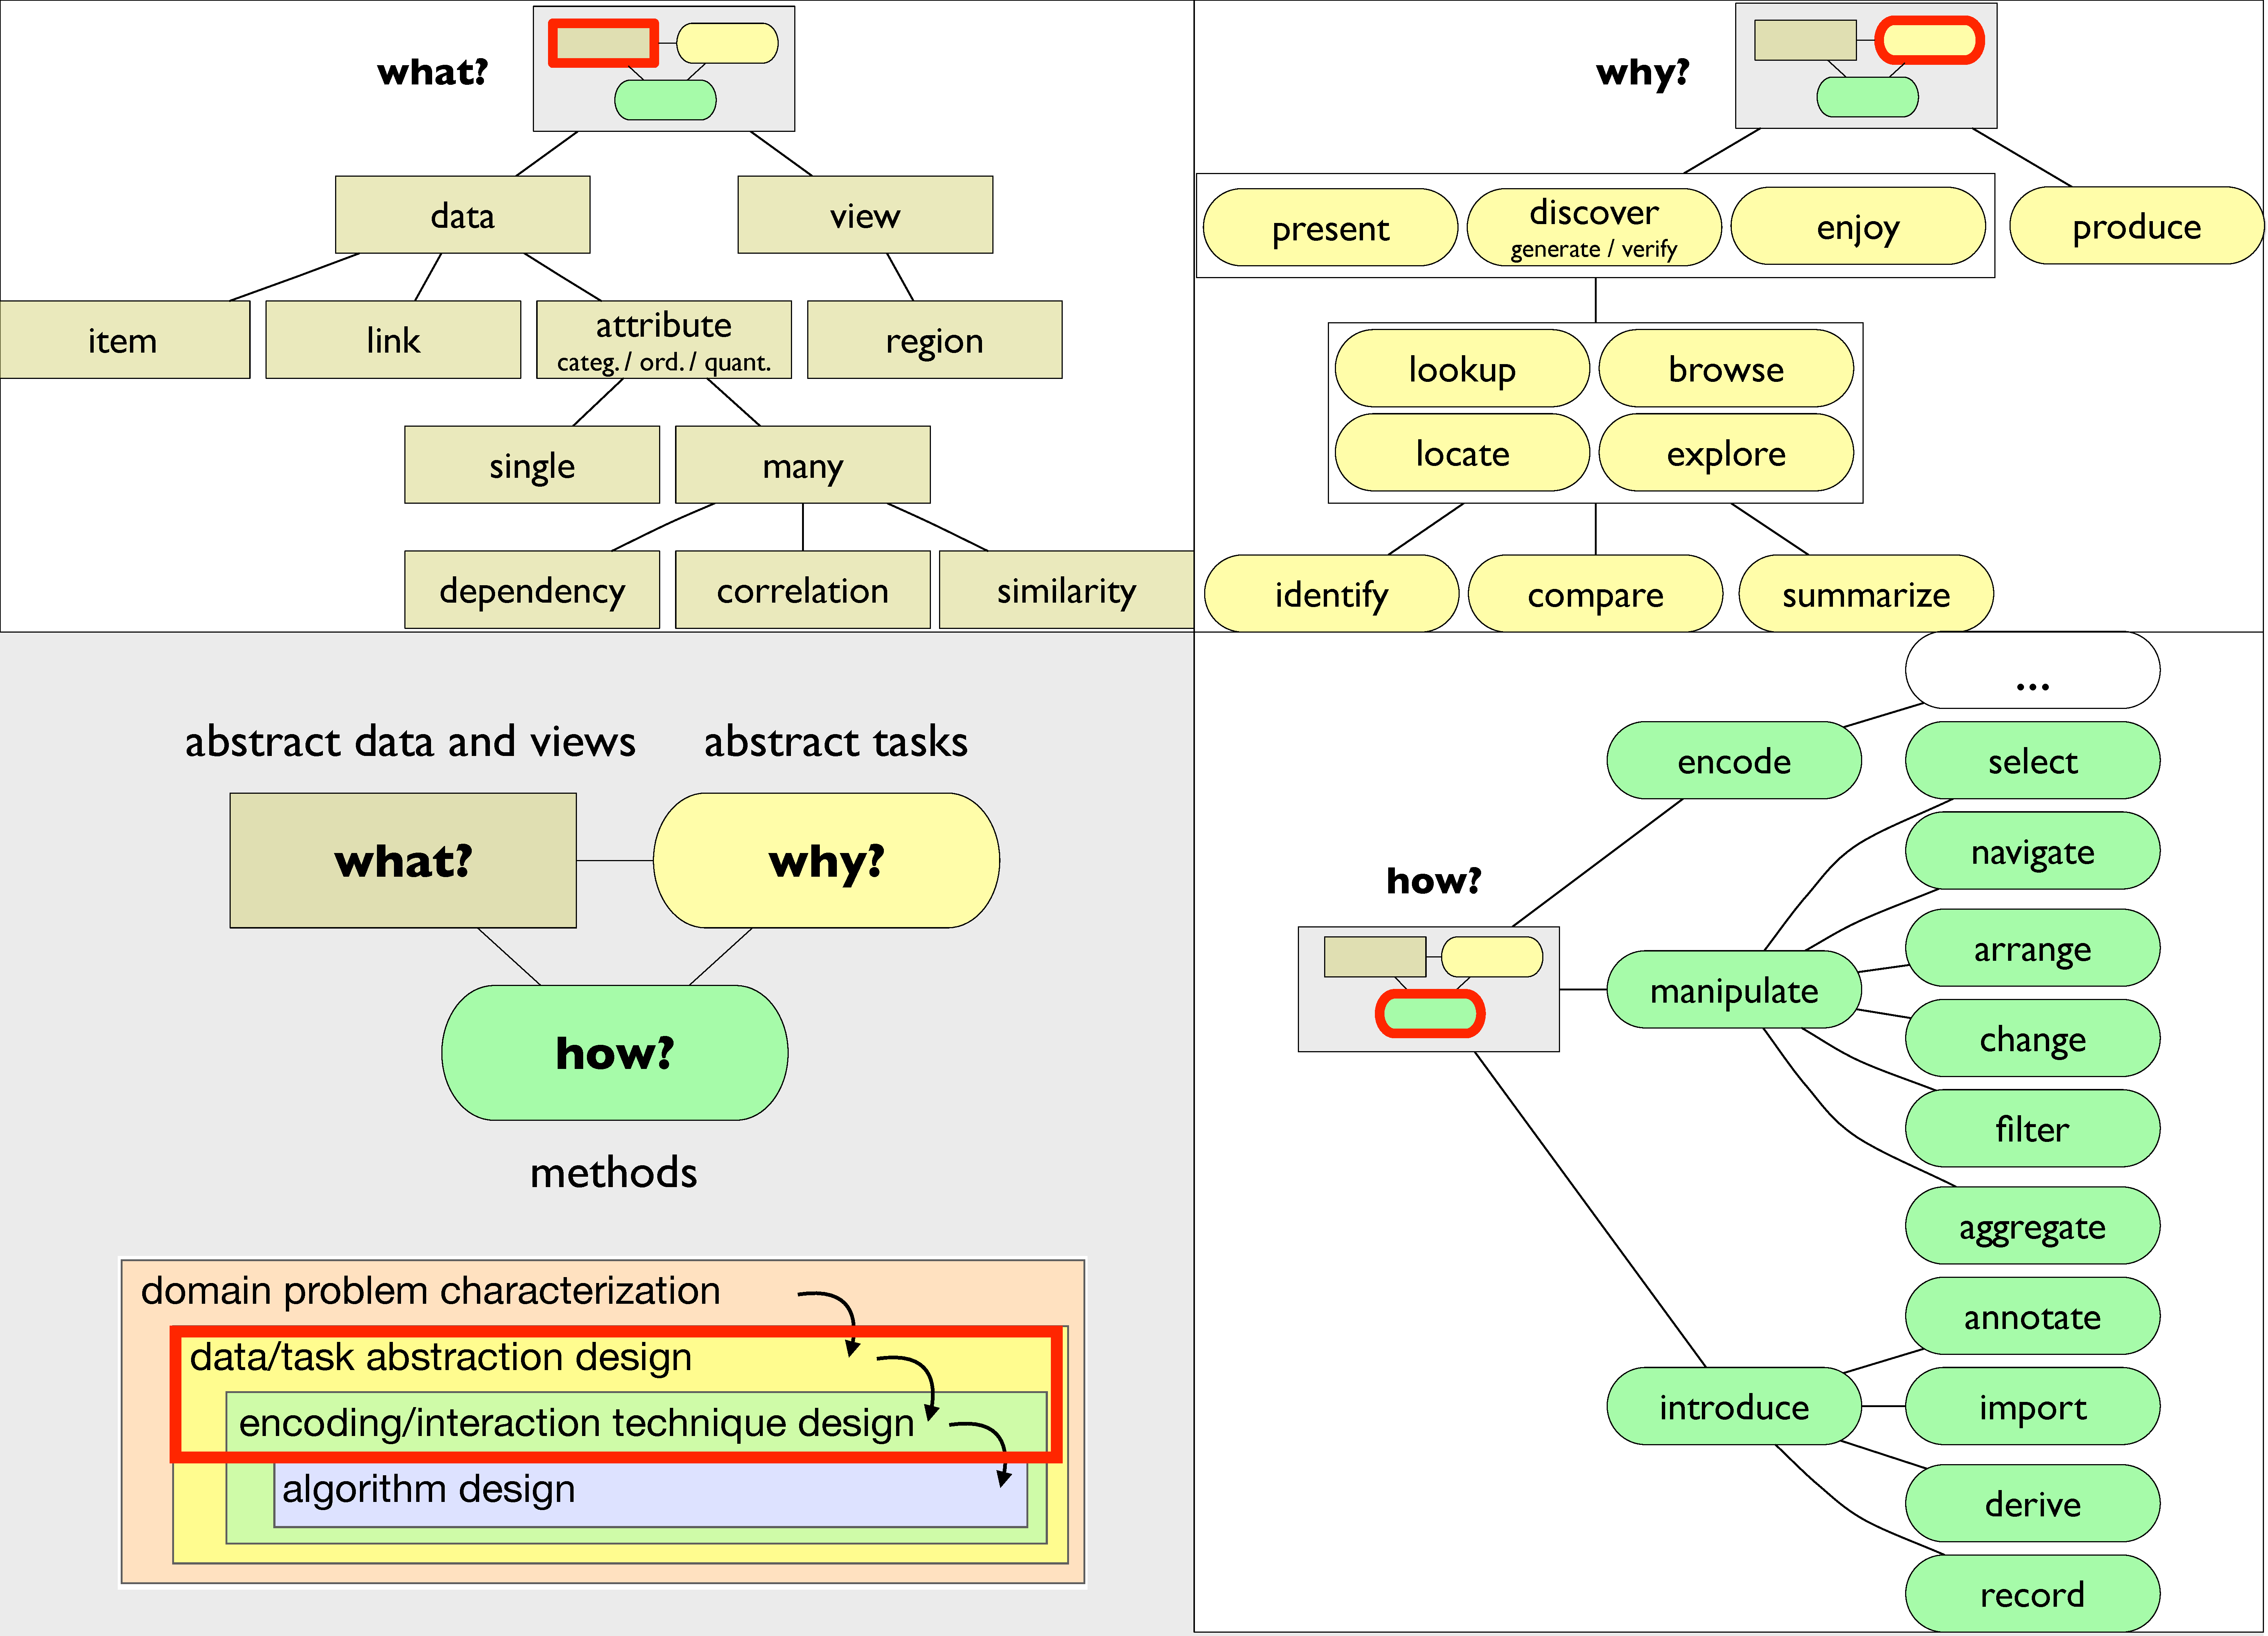
\includegraphics[width=0.975\textwidth]{figures/typology-13-02-25.pdf}
	\caption
	[
	    Our sixth classification.
	]
	{
	    {\bf February 25, 2013}: Our sixth classification, which simplifies our characterization of single attributes and makes the connection to Munzner's nested model~\cite{Munzner2009} more explicit.
	}
	\centering
	\label{app:typology:fig:13.02.25}
\end{figure}

%-|-|-|-|-|-|-|-|-|-|-|-|-|-|-|-|-|-|-|-|-|-|-|-|-|-|-|-|-|-|-|-|-|-|-|-|-

\bstart{March 4, 2013}
The UBC InfoVis group along with visitor Colin Ware met to discuss our draft: {\it``Mid-Level Tasks for Visualization Design and Evaluation''}.

The group's critique included: (i) they disputed the term {\it mid-level} since we had multiple levels in our classification, and though the {\it why-what-how} division was appreciated (with the strengths being {\it why} and {\it how}), our classification of {\it what} was disputed and was thought to be underdeveloped; (ii) they acknowledged our abundance of motivation but suggested that many readers may not appreciate this motivation without additional context (beyond the Nested Model~\cite{Munzner2009}\index{nested model (Munzner)}), running examples, and use cases; (iii) our claims of {\it evaluative} and {\it generative} power were disputed, as were our claims regarding that our work was {\it actionable} and {\it persuasive}; (iv) some of our task description examples were expressed with a pseudocode-like notation, which was deemed to be confusing, and it was similarly it was unclear as to why we presented the terminology of related work in a table (referring to \autoref{typology:tab:rw:why} and \autoref{typology:tab:rw:how}); (v) finally, they asked us to be more explicit with regards to what was gained with the advent of our classification and why ours was superior to all prior classifications.
%-------------------------------------------------------------------------

\section{Our Proposed Taxonomy of Tasks}
\label{app:typology:chronology:proposed}

%-------------------------------------------------------------------------

\bstart{March 13, 2013}
Our seventh classification is shown in \autoref{app:typology:fig:13.03.13}; this classification is identical to the typology as it is presented in \autoref{ch:typology} (reproduced in \autoref{app:typology:fig:typology} below) in all aspects save its visual layout, which includes an illustration of a sequence of interdependent tasks\index{task!task sequence}.
In response to feedback from UBC InfoVis group readers and to our recent reading of \citet{Tweedie1997}, we drastically simplified our classification of {\it what} to an even greater extent, reducing it to {\tt input} and {\tt output}.
We also started to refer to our classification as a {\it multi-level taxonomy} as opposed to one classifying {\it mid-level tasks}\index{task!mid-level tasks}. 
We emphasized our taxonomy as resulting from a combination of literature review and new thinking.
We cut back on our discussion of {\it evaluative} and {\it generative} potential, emphasizing the {\it descriptive} power of our classification.
We also dropped the discussion of whether our classification was {\it actionable} or {\it persuasive}~\cite{Gleicher2012}.

%-|-|-|-|-|-|-|-|-|-|-|-|-|-|-|-|-|-|-|-|-|-|-|-|-|-|-|-|-|-|-|-|-|-|-|-|-

\begin{figure}
	\centering
	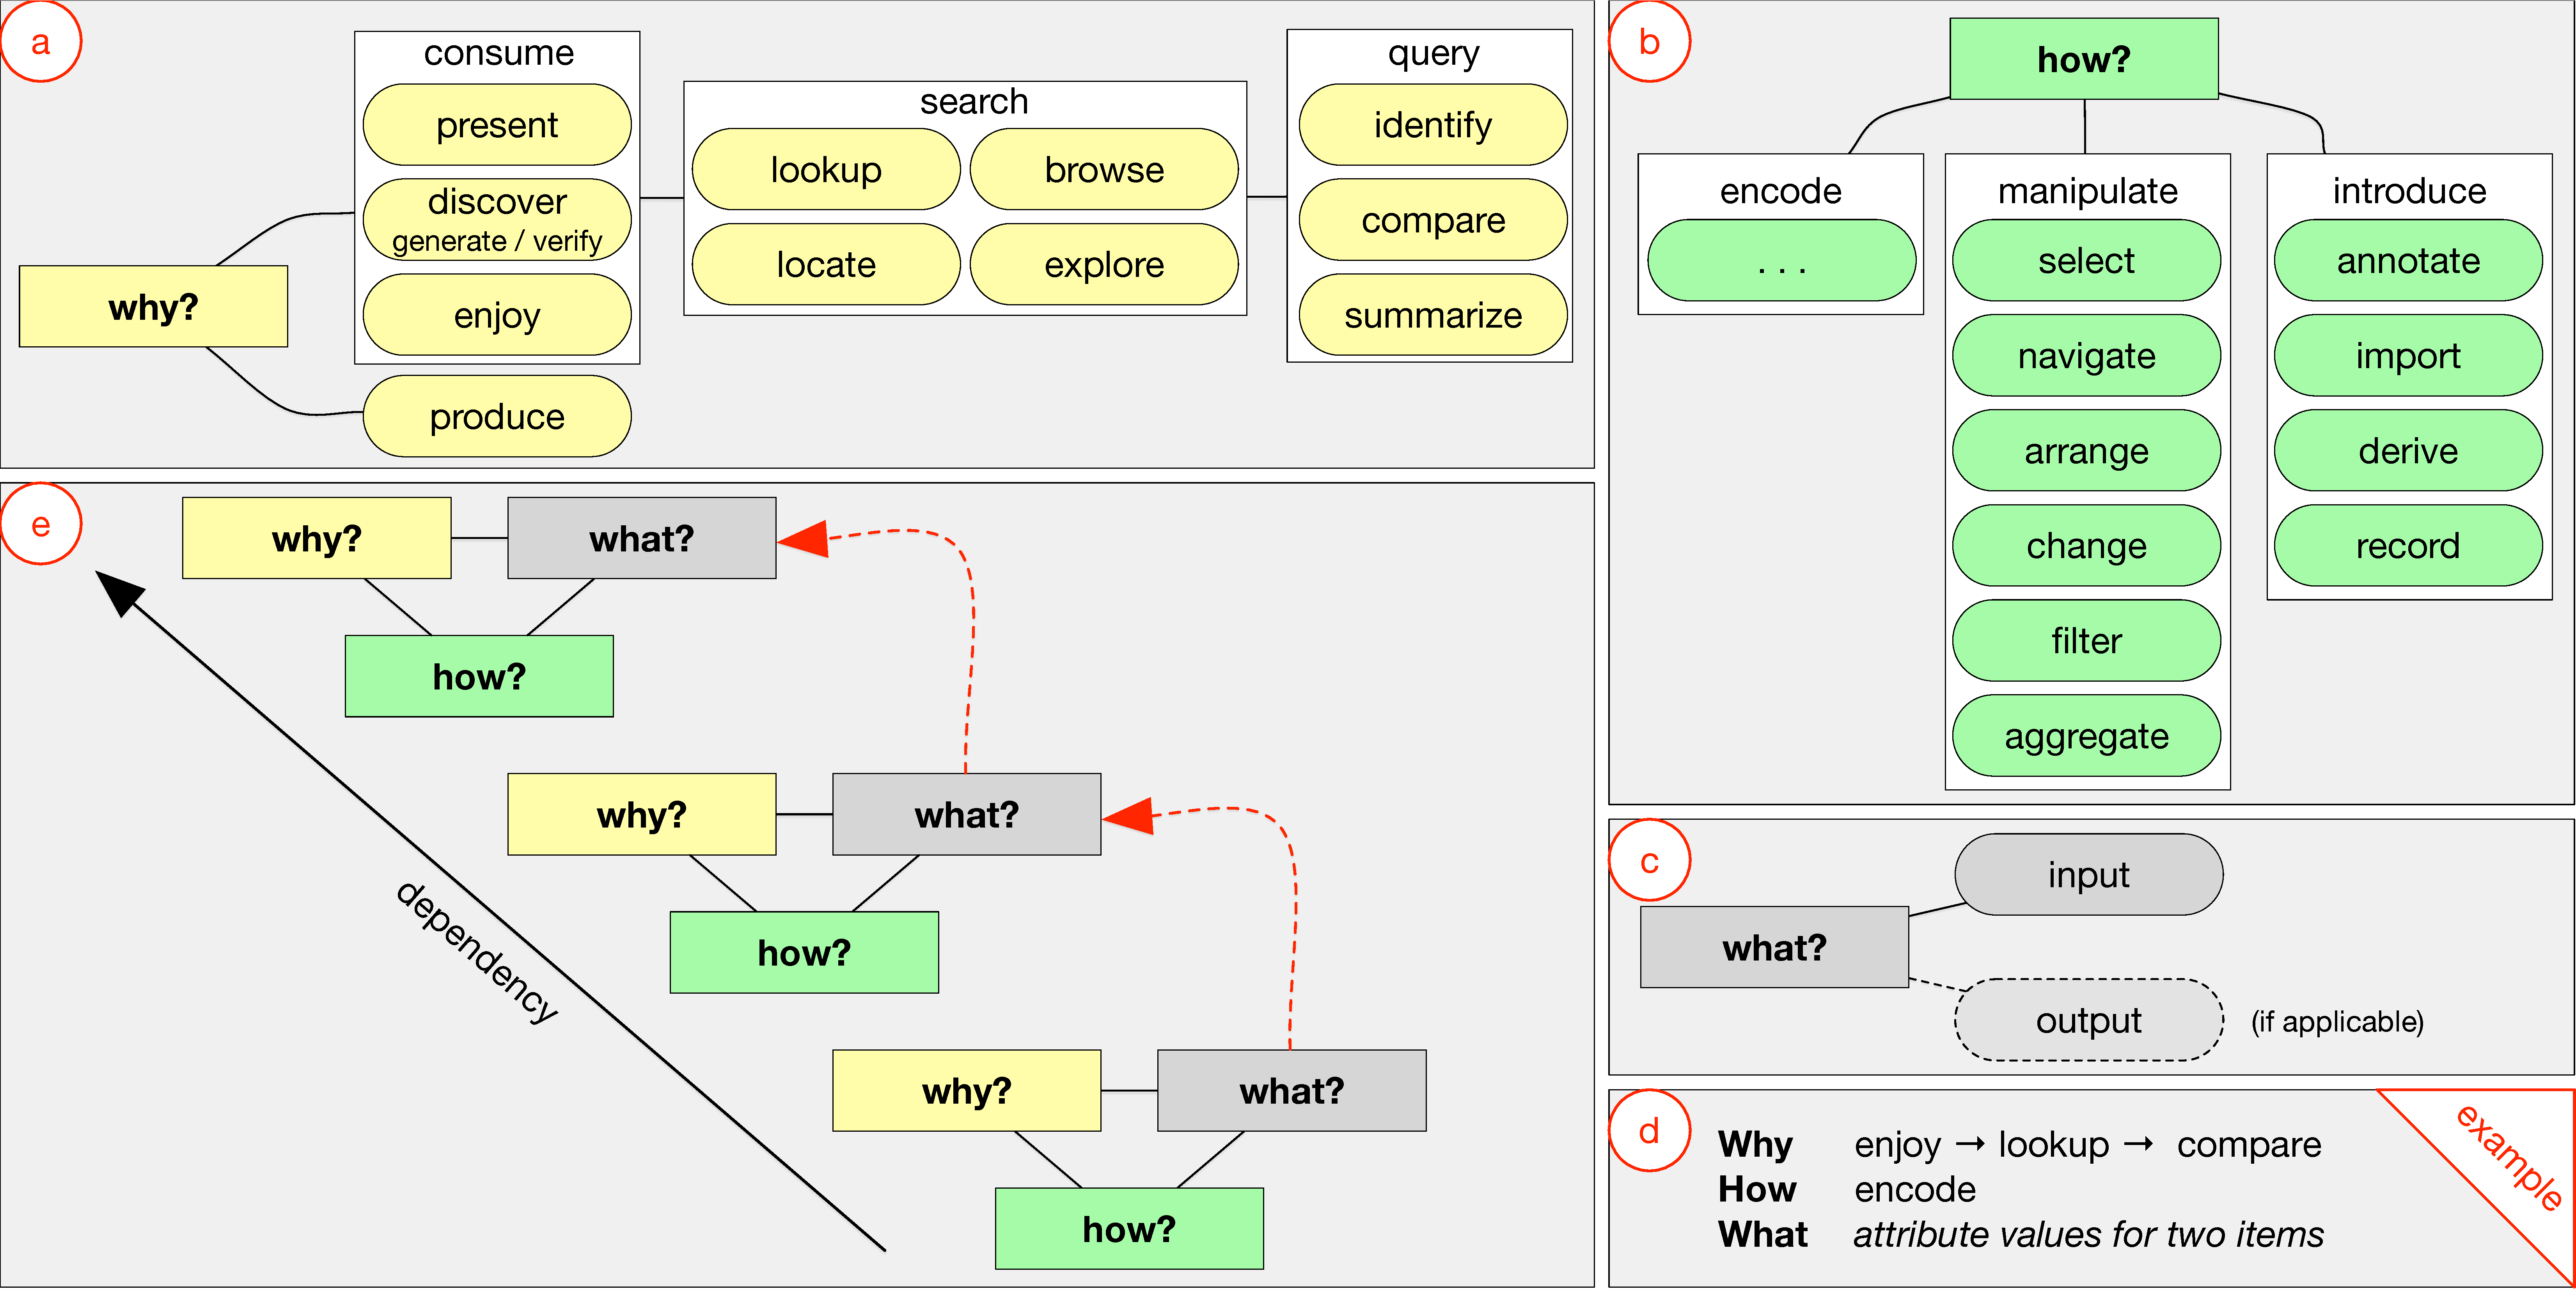
\includegraphics[width=\textwidth]{figures/typology-13-03-13.pdf}
	\caption
	[
	    Our seventh and proposed classification.
	]
	{
	    {\bf March 13, 2013}: Our seventh and proposed classification, including a simplification of \textsl{what}: (a) \textsl{why} a task is performed; (b) \textsl{how} the task is supported; (c) \textsl{what} are the {\tt inputs} and {\tt outputs} of the task; (d) an example task description; (e) a sequence of interdependent tasks.
	}
	\centering
	\label{app:typology:fig:13.03.13}
\end{figure}

%-|-|-|-|-|-|-|-|-|-|-|-|-|-|-|-|-|-|-|-|-|-|-|-|-|-|-|-|-|-|-|-|-|-|-|-|-

\bstart{March 31, 2013}
Submission of {\it``A Multi-Level \underline{Taxonomy} of Abstract Visualization Tasks''} to IEEE Information Visualization.

%-------------------------------------------------------------------------

\section{Revisions: From Taxonomy to Typology}
\label{app:typology:chronology:taxonomy}

%-------------------------------------------------------------------------

\bstart{June 6, 2013}
{\it``A Multi-Level Taxonomy of Abstract Visualization Tasks''} was conditionally accepted to IEEE Information Visualization, and we revisited our literature review in response to the anonymous reviews.

\refstepcounter{papernumber} 
\begin{sloppypar}
\bstart{June 10, 2013\thepapernumber}
\bibentry{Aigner2011}~\cite{Aigner2011}. \end{sloppypar}

\begin{quotation}
    Recommended by an anonymous reviewer and makes compelling or noteworthy assertions about the behaviour of people who use time-oriented\index{time-oriented data} visualization tools or techniques.
    
    Includes an analysis framework centred around {\it why}, {\it what}, and {\it how}, asking {\it what is presented?}, {\it why is it presented?}, and {\it how is it presented?} (implying a focus on visual encodings\index{visual encoding}).
    
    Also includes {\it time-oriented primitives}\index{time-oriented data} that we cite in reference to {\it what}, which includes {\it points, intervals, spans, temporal patterns, rates of change, sequences}, and {\it synchronization}.
    
    They also refer to classifications by \citet{Andrienko2006}, \citet{Spence2007}, and \citet{Yi2007}. 
    The authors to higher-level analysis tasks\index{task} to which visualization of time-oriented data contributes to, which includes {\it classification, clustering, search, retrieval, pattern discovery}, and {\it prediction}.
\end{quotation}

\refstepcounter{papernumber} 
\begin{sloppypar}
\bstart{June 10, 2013\thepapernumber}
\bibentry{Ware2012}~\cite{Ware2012}. \end{sloppypar}

\begin{quotation}
    In addition to the content carried over from the 2nd edition (\citet{Ware2004}, see \autoref{app:typology:chronology:dedicated}), Ware contributes a high-level classification\index{task!high-level tasks}, adding ten {\it visual thinking algorithms} in the 3rd edition, which include {\it visual queries}, {\it pathfinding on a map or diagram}, {\it reasoning with a hybrid of a visual display and mental imagery}, {\it design sketching}, {\it brushing}\index{view coordination!brushing across views}, {\it small pattern comparisons in a large information space}, {\it degree-of-relevance highlighting}, {\it generalized fisheye views}, {\it multidimensional dynamic queries with scatterplot\index{visual encoding!scatterplot}}, and {\it visual monitoring strategies}.
\end{quotation}

\refstepcounter{papernumber} 
\begin{sloppypar}
\bstart{June 10, 2013\thepapernumber}
\bibentry{Andrienko2006}~\cite{Andrienko2006}. \end{sloppypar}

\begin{quotation}
    Recommended by an anonymous reviewer and contributes a low-level classification\index{task!low-level tasks} that distinguishes between {\it elementary} and {\it synoptic} tasks (inspired by the {\it  elementary, intermediate}, and {\it overall levels of reading} described by \citet{Bertin2011}), as well as {\it references} and {\it characteristics}.
    
    {\it Elementary tasks} include {\it direct lookup} ({\it identification}), {\it inverse lookup} ({\it localization}), {\it direct comparison} ({\it identification and interrelation of characteristics}), {\it inverse comparison} ({\it localization and interrelation of references}), and {\it relation seeking}. 
    
    {\it Synoptic tasks} include {\it descriptive tasks} ({\it direct lookup / pattern definition and identification, inverse lookup / pattern search and localization, direct pattern comparison, inverse pattern comparison, relation seeking}) and {\it connectional tasks} ({\it identify heterogeneous behaviour, identify homogeneous behaviour}).
    
    \begin{sloppypar}
    Includes a formal quasi-algebraic notation for specifying these tasks in terms of {\it referents} ({\it points}) and {\it characteristics} ({\it attributes}).
    \end{sloppypar}
    
    The authors define a task\index{task} as having two parts: a {\it target} ({\it what information needs to be obtained}) and {\it constraints} ({\it what conditions this information needs to fulfil}). 
    Targets for synoptic tasks\index{task} are types of patterns or configurations of {\it characteristics} for a {\it reference set}; they include: {\it association, differentiation, arrangement}, and {\it distribution summary}. 
\end{quotation}

\refstepcounter{papernumber} 
\begin{sloppypar}
\bstart{June 10, 2013\thepapernumber}
\bibentry{Lammarsch2012}~\cite{Lammarsch2012}. \end{sloppypar}

\begin{quotation}
    Recommended by an anonymous reviewer for connecting the {\it what} to the {\it how}; contributes a datatype specific classification of tasks relating to time-oriented data\index{time-oriented data}, extending the top-down task classification for spatial and temporal data by \citet{Andrienko2006}, introducing a formal notation for specifying these tasks and incorporating the time-oriented\index{time-oriented data} primitives introduced by \citet{Aigner2011}: {\it scale, scope, arrangement, viewpoints} ({\it ordered} vs. {\it branching time}), {\it granularities}, and {\it determinancy}.
\end{quotation}

\refstepcounter{papernumber} 
\begin{sloppypar}
\bstart{June 10, 2013\thepapernumber}
\bibentry{Raskin2000}~\cite{Raskin2000}. \end{sloppypar}

\begin{quotation}
    Recommended by an anonymous reviewer in response to the {\tt manipulate} nodes in our {\it how} classification, and contributes a low-level classification\index{task!low-level tasks}, a {\it taxonomy of elementary actions} that might be performed with a mouse and keyboard.
    Raskin's classification is addressed at an \ac{HCI}\index{human-computer interaction (HCI)} readership, though his classification applies to many visualization tools.
    
    Rasking distinguishes between {\it indicating} ({\it pointing}), {\it selecting, activating}, and {\it modifying} ({\it or using: generating, deleting, moving, transforming, copying}). 
\end{quotation}

\refstepcounter{papernumber} 
\begin{sloppypar}
\bstart{June 13, 2013\thepapernumber}
\bibentry{Dork2011}~\cite{Dork2011}. \end{sloppypar}

\begin{quotation}
    \begin{sloppypar}
    Makes compelling or noteworthy assertions about the behaviour of people who use visualization artefacts in casual contexts, including curiosity-driven tasks without expectations or predicted outcomes, where novelty stimulates curiosity and thereby exploration.
    \end{sloppypar}
    
    Added in response to an anonymous reviewer who indicated that our term {\tt enjoy}\index{{\tt enjoy}} was somewhat vague.
\end{quotation}

\refstepcounter{papernumber} 
\begin{sloppypar}
\bstart{June 13, 2013\thepapernumber}
\bibentry{Dork2012}~\cite{Dork2012}. \end{sloppypar}

\begin{quotation}
    Makes compelling or noteworthy assertions about the behaviour of people who use visualization artefacts in casual contexts in which the information being visualized is simply enjoyed; introduces the concept of {\it strolling} through information spaces, and discusses the characteristics of {\it browsing} and {\it searching}.
    
    Added in response to an anonymous reviewer who indicated that our term {\tt enjoy}\index{{\tt enjoy}} was somewhat vague.
\end{quotation}

\refstepcounter{papernumber} 
\begin{sloppypar}
\bstart{June, 2013\thepapernumber}
\bibentry{Pousman2007}~\cite{Pousman2007}. \end{sloppypar}

\begin{quotation}
    Makes compelling or noteworthy assertions about the behaviour of people who use visualization artefacts in casual contexts in which the information being visualized is simply enjoyed,  including immersive and time-consuming experiences, such as in museum settings.
    
    Added in response to an anonymous reviewer who indicated that our term {\tt enjoy}\index{{\tt enjoy}} was somewhat vague.
\end{quotation}

\refstepcounter{papernumber} 
\begin{sloppypar}
\bstart{June 18, 2013\thepapernumber}
\bibentry{Smith2002}~\cite{Smith2002}. \end{sloppypar}

\begin{quotation}
    Smith indicates that ``{\it the key characteristic of a typology is that its dimensions represent concepts rather than empirical cases [and that] typologies create useful heuristics and provide a systematic basis for comparison \ldots Their central drawbacks are categories that are neither exhaustive nor mutually exclusive}.''
    Taxonomies, on the other hand, ``{\it classify items on the basis of empirically observable and measurable characteristics}.''

    Considered in response an anonymous reviewer who questioned whether we had truly proposed a {\it taxonomy}, implying completeness, indicating that others have use the less strict {\it typology} in this context; we did not cite this work in \autoref{ch:typology} or \citet{Brehmer2013}, opting to cite the original source  \citet{Bailey1994} instead.
\end{quotation}

\refstepcounter{papernumber} 
\begin{sloppypar}
\bstart{June 18, 2013\thepapernumber}
\bibentry{Bailey1994}~\cite{Bailey1994}. \end{sloppypar}

\begin{quotation}
    Bailey indicates that a {\it typology} is appropriate for classifying abstract concepts, while a {\it taxonomy} is appropriate for classifying empirically observable events and are often but not always hierarchical.

    Added in response an anonymous reviewer who questioned whether we had proposed a {\it taxonomy}, or a {\it typology}.
\end{quotation}

\refstepcounter{papernumber} 
\begin{sloppypar}
\bstart{June 19--27, 2013\thepapernumber}
\bibentry{Vicente1999}~\cite{Vicente1999}. \end{sloppypar}

\begin{quotation}
    Recommended by an anonymous reviewer who stated that ``{\it The authors will enjoy it}''\footnote{I did enjoy it; thanks R3!}.
    
    Describes {\it cognitive work analysis}\index{cognitive work analysis (Vicente)}, a framework that combines {\it constraint-based task analysis} with {\it work domain analysis}\index{work domain analysis} as the ``{\it foundation for a holistic and socio-technical account of a person's work involving information technology}'', which involves five phases: {\it work domain analysis\index{work domain analysis}, control task analysis, strategies analysis, social organization and cooperation analysis}, and {\it worker competencies analysis}. 
    
    Vicente contrasts {\it normative work analysis} (how work {\it should} be done), {\it descriptive work analysis} (how work {\it is} done, including workarounds and strategies outside of what is prescribed by the normative account of the work), and {\it cognitive work analysis}\index{cognitive work analysis (Vicente)} as a form of {\it formative work analysis} (how work {\it could} be done, subject to known constraints, such as {\it inputs} and {\it outputs}, social organization, and worker competencies). 
    
    The {\it strategies analysis} phase involves describing {\it how} a task is carried out independent of who does it, still in a device-agnostic fashion, examining the different possible strategies by which the task could be executed.
    
    Like us, Vicente appreciates the power and simplicity of asking {\it why, what}, and {\it how} for elucidating {\it means} and {\it ends}, though he is referring to the {\it structural means-ends} relations in a work domain's {\it abstraction hierarchy}, while we are concerned with {\it action means-ends relations} of tasks; in other words, relations between nouns vs. relations between verbs. 
    Finally, Vicente argues that sequence-based approaches to task analysis\index{task!task analysis} are overly rigid and thus inappropriate for describing such open-ended tasks; {\it constraint}-based approaches to task analysis\index{task!task analysis} allow for more flexibility in terms of {\it how}\index{{\tt how}} a task\index{task} is performed.
\end{quotation}

\bstart{June 27, 2013}
Submission of a revision to IEEE Information Visualization, which we renamed {\it``A Multi-Level \underline{Typology} of Abstract Visualization Tasks''}.
In addition to opting to use the term {\it typology} and including the recommended references, we extended the definition for each node of our typology, now including one or more succinct examples, and we also made an effort to disambiguate the terminology flagged by reviewers. 
We added a section providing background context (\autoref{typology:context}) to outline the limitations faced by practitioners conducting task analysis, that previous classifications cannot be used to generate concise and abstract task descriptions needed for design and evaluation. 
Finally, we extended our discussion of {\it what} to include several illustrative example classifications of {\it what} as proposed by previous work (see \autoref{typology:what}).

%-------------------------------------------------------------------------

\section{Presenting our Typology}
\label{app:typology:chronology:presentation}

%-------------------------------------------------------------------------

\bstart{July 11, 2013}
{\it``A Multi-Level Typology of Abstract Visualization Tasks''} was accepted to IEEE Information Visualization.

\bstart{August 1, 2013}
We submitted a camera-ready version of {\it``A Multi-Level Typology of Abstract Visualization Tasks''} to IEEE Information Visualization.
In this revision, we responded to the meta-reviewer's comments regarding the presentation of the typology in \autoref{app:typology:fig:typology}, clarifying the differences between {\tt discover}\index{{\tt discover}} types {\it generate hypotheses} and {\it verify hypotheses}, the {\it means} and {\it ends} of {\tt produce}\index{{\tt produce}}, the scope of {\tt change}\index{{\tt change}}, and the difference between {\tt annotate} (a verb: {\it how}) and an annotation (a noun: {\it what}).
We also highlighted terms from previous work relating to {\it what} in \autoref{typology:tab:rw:why} and \autoref{typology:tab:rw:how} using parentheses.

% \refstepcounter{papernumber} 
% \begin{sloppypar}
% \bstart{September 30, 2013\thepapernumber}
% \bibentry{Roth2013}~\cite{Roth2013}. \end{sloppypar}

% \begin{quotation}
%     A longer journal version of the 2012 workshop paper discussed above~\cite{Roth2012}, appearing in the ``Defining the design space'' InfoVis session of InfoVis 2013 alongside our paper.
% \end{quotation}

% \refstepcounter{papernumber} 
% \begin{sloppypar}
% \bstart{August 2, 2013\thepapernumber}
% \bibentry{Schulz2013}~\cite{Schulz2013}. \end{sloppypar}

% \begin{quotation}
%     Appeared in the ``Defining the design space'' InfoVis session of InfoVis 2013 alongside our paper.
    
%     Introduces a design space for specifying tasks\index{task}, with dimensions {\it why}, {\it how}, and {\it what}, as well as {\it where} does a task\index{task} operate in the data, {\it when} a task\index{task} is performed, and {\it who} is executing the task\index{task}. 
%     They also introduce a formal notation for describing tasks, and they realize their design space with an implementation of a tool for recommending visualization techniques in relation to climate impact data.
% \end{quotation}

\bstart{October 13--18, 2013}
I attended the 2013 IEEE VIS Conference and presented {\it``A Multi-Level Typology of Abstract Visualization Tasks''} in the ``Defining the design space'' InfoVis session, which also included task\index{task} classification papers by \citet{Schulz2013} and \citet{Roth2013}.
Roth's paper was a longer journal version of his 2012 {\it GIScience} workshop paper discussed above~\cite{Roth2012}; his classification remain unchanged.
I comment upon the differences between our typology and ``{\it A Design Space of Visualization Tasks}'' by \citet{Schulz2013} in \autoref{conclusions:typology:contemporary}.
I presented the typology as it is shown in \autoref{ch:typology} and in \autoref{app:typology:fig:typology}; we omitted the illustration of a sequence of interdependent tasks\index{task!task sequence} due to space constraints.
Finally, \autoref{app:typology:fig:slides-4} is one aspect of our meta-analysis of existing classifications that I presented at IEEE VIS 2013.

%-|-|-|-|-|-|-|-|-|-|-|-|-|-|-|-|-|-|-|-|-|-|-|-|-|-|-|-|-|-|-|-|-|-|-|-|-


\begin{figure}
    \centering
    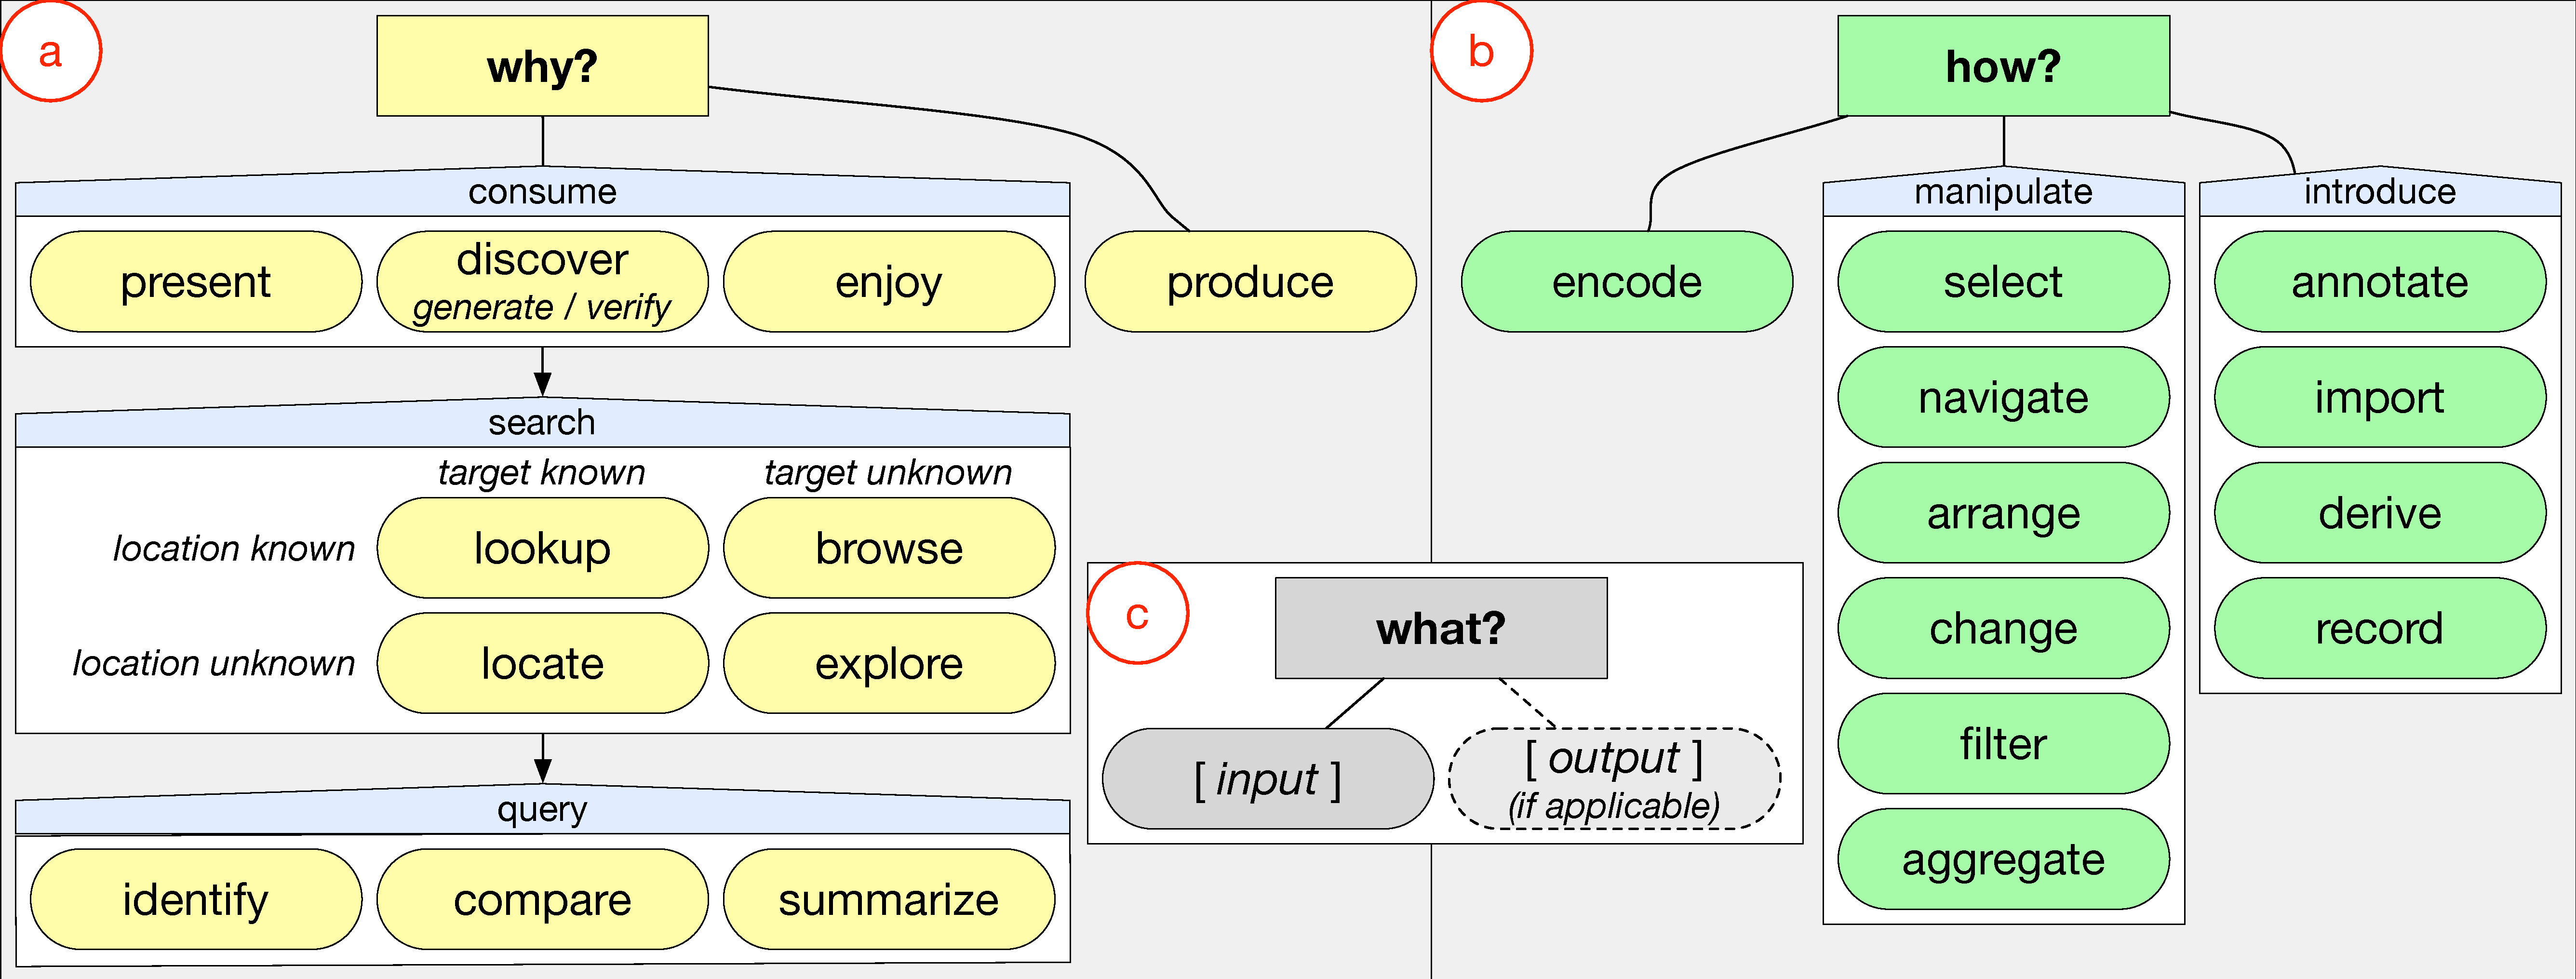
\includegraphics[width=\textwidth]{figures/typology.pdf}
    \caption
    [
        Our multi-level typology of abstract visualization tasks as of October 2013.
    ]
    {
        {\bf October 13--18, 2013}: Our multi-level typology of abstract visualization tasks as it was presented in \autoref{ch:typology} and at IEEE VIS 2013.
    }
    \label{app:typology:fig:typology}
\end{figure}

%-|-|-|-|-|-|-|-|-|-|-|-|-|-|-|-|-|-|-|-|-|-|-|-|-|-|-|-|-|-|-|-|-|-|-|-|-

%-|-|-|-|-|-|-|-|-|-|-|-|-|-|-|-|-|-|-|-|-|-|-|-|-|-|-|-|-|-|-|-|-|-|-|-|-

\begin{figure}
	\centering
	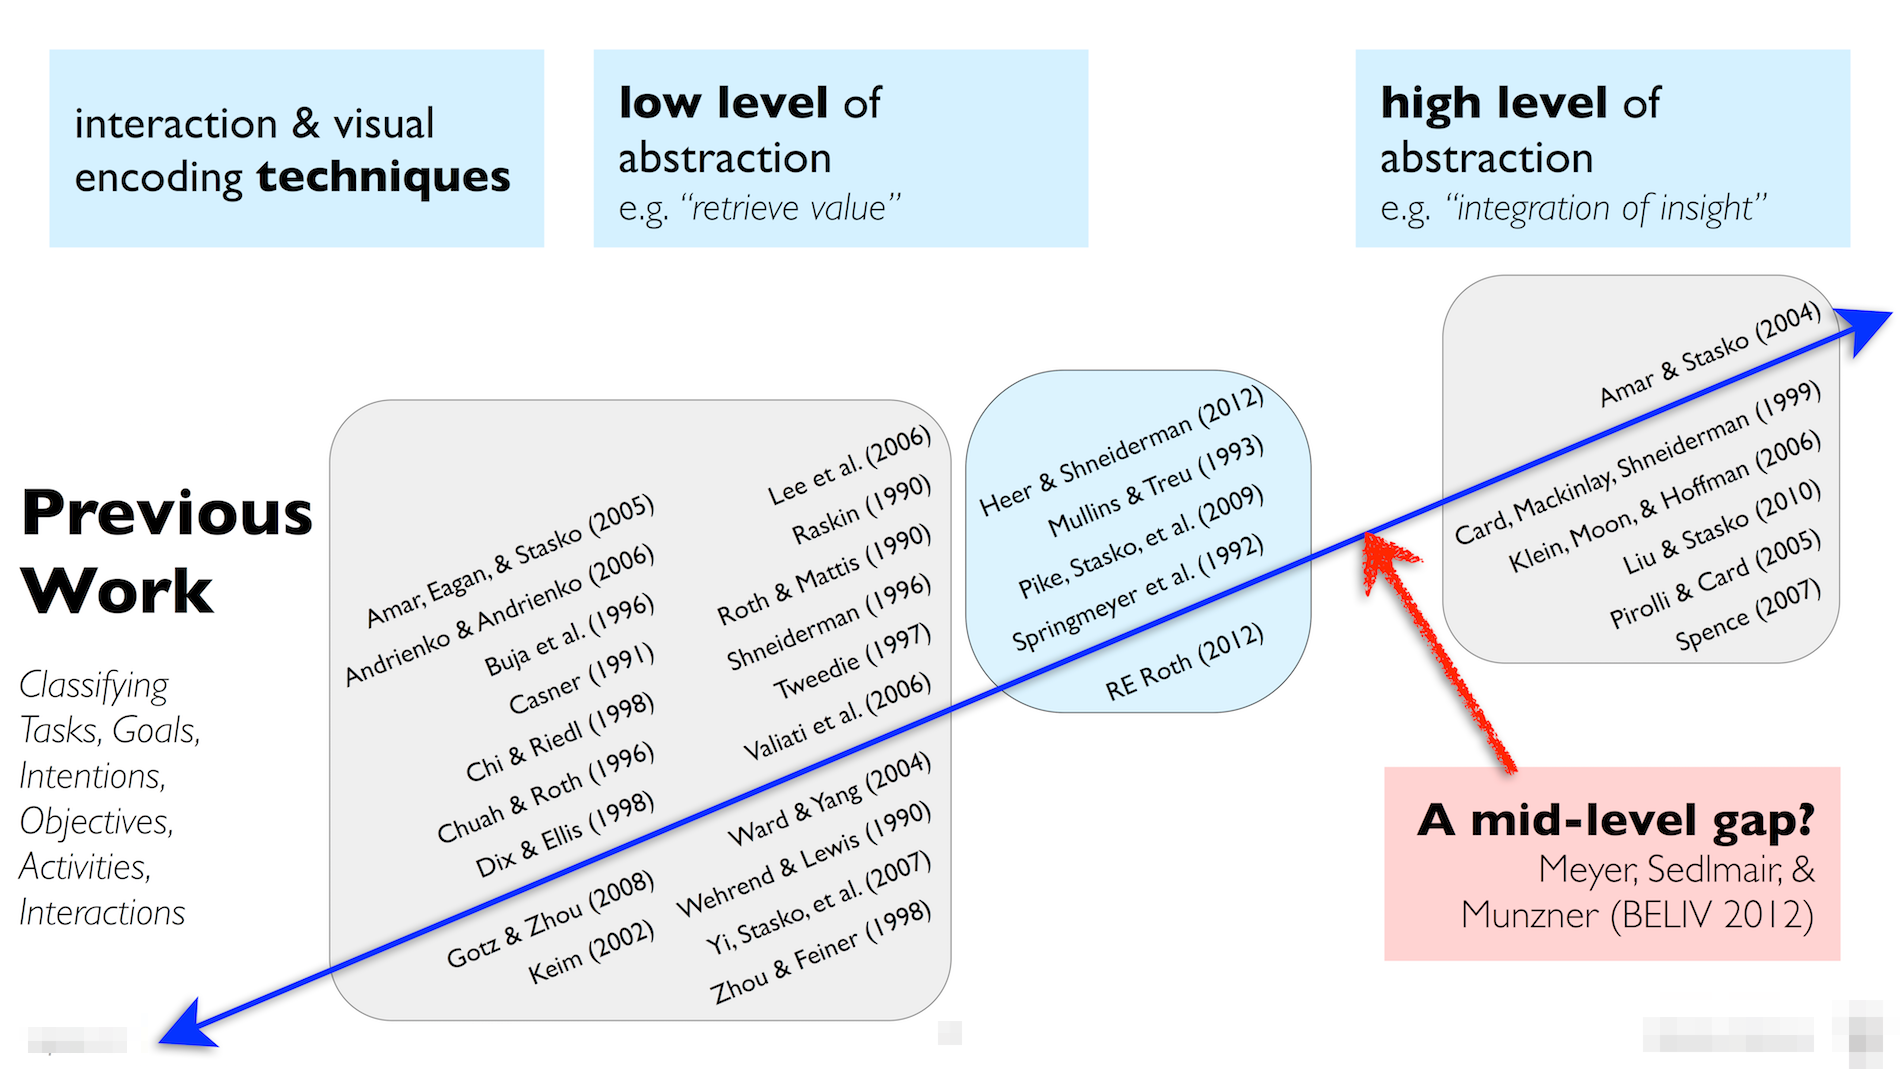
\includegraphics[width=\textwidth]{figures/typology-slides-4.png}
	\caption
	[
	    Previous classifications sorted from low to high level of abstraction.
	]
	{
	    {\bf October 13--18, 2013}: Previous classifications sorted from low to high level of abstraction, highlighting a mid-level gap; one aspect of our meta-analysis of existing classifications that we presented at IEEE VIS 2013.
	}
	\centering
	\label{app:typology:fig:slides-4}
\end{figure}

%-|-|-|-|-|-|-|-|-|-|-|-|-|-|-|-|-|-|-|-|-|-|-|-|-|-|-|-|-|-|-|-|-|-|-|-|-

%-------------------------------------------------------------------------

\section{Subsequent Evolution of our Typology}
\label{app:typology:chronology:evolution}

%-------------------------------------------------------------------------

\bstart{Summer 2014}
Tamara continued to iterate on the typology\index{task!task typology} as she completed her book~\cite{Munzner2014}.
The version of the typology\index{task!task typology} that appears in her book is reproduced in \autoref{conclusions:typology}, where I also indicate and reflect upon the differences between the version of the typology\index{task!task typology} presented at IEEE InfoVis 2013 and the version in her book. 